% Options for packages loaded elsewhere
\PassOptionsToPackage{unicode}{hyperref}
\PassOptionsToPackage{hyphens}{url}
%
\documentclass[
]{memoir}
\usepackage{amsmath,amssymb}
\usepackage{lmodern}
\usepackage{iftex}
\ifPDFTeX
  \usepackage[T1]{fontenc}
  \usepackage[utf8]{inputenc}
  \usepackage{textcomp} % provide euro and other symbols
\else % if luatex or xetex
  \usepackage{unicode-math}
  \defaultfontfeatures{Scale=MatchLowercase}
  \defaultfontfeatures[\rmfamily]{Ligatures=TeX,Scale=1}
  \setmainfont[]{Roboto}
  \setsansfont[]{Clancy}
  \setmonofont[Scale=0.9]{Roboto Mono}
\fi
% Use upquote if available, for straight quotes in verbatim environments
\IfFileExists{upquote.sty}{\usepackage{upquote}}{}
\IfFileExists{microtype.sty}{% use microtype if available
  \usepackage[]{microtype}
  \UseMicrotypeSet[protrusion]{basicmath} % disable protrusion for tt fonts
}{}
\makeatletter
\@ifundefined{KOMAClassName}{% if non-KOMA class
  \IfFileExists{parskip.sty}{%
    \usepackage{parskip}
  }{% else
    \setlength{\parindent}{0pt}
    \setlength{\parskip}{6pt plus 2pt minus 1pt}}
}{% if KOMA class
  \KOMAoptions{parskip=half}}
\makeatother
\usepackage{xcolor}
\IfFileExists{xurl.sty}{\usepackage{xurl}}{} % add URL line breaks if available
\IfFileExists{bookmark.sty}{\usepackage{bookmark}}{\usepackage{hyperref}}
\hypersetup{
  pdftitle={PHCM9795 Foundations of Biostatistics},
  pdfauthor={Pilot Notes for R},
  hidelinks,
  pdfcreator={LaTeX via pandoc}}
\urlstyle{same} % disable monospaced font for URLs
\usepackage{color}
\usepackage{fancyvrb}
\newcommand{\VerbBar}{|}
\newcommand{\VERB}{\Verb[commandchars=\\\{\}]}
\DefineVerbatimEnvironment{Highlighting}{Verbatim}{commandchars=\\\{\}}
% Add ',fontsize=\small' for more characters per line
\usepackage{framed}
\definecolor{shadecolor}{RGB}{248,248,248}
\newenvironment{Shaded}{\begin{snugshade}}{\end{snugshade}}
\newcommand{\AlertTok}[1]{\textcolor[rgb]{0.94,0.16,0.16}{#1}}
\newcommand{\AnnotationTok}[1]{\textcolor[rgb]{0.56,0.35,0.01}{\textbf{\textit{#1}}}}
\newcommand{\AttributeTok}[1]{\textcolor[rgb]{0.77,0.63,0.00}{#1}}
\newcommand{\BaseNTok}[1]{\textcolor[rgb]{0.00,0.00,0.81}{#1}}
\newcommand{\BuiltInTok}[1]{#1}
\newcommand{\CharTok}[1]{\textcolor[rgb]{0.31,0.60,0.02}{#1}}
\newcommand{\CommentTok}[1]{\textcolor[rgb]{0.56,0.35,0.01}{\textit{#1}}}
\newcommand{\CommentVarTok}[1]{\textcolor[rgb]{0.56,0.35,0.01}{\textbf{\textit{#1}}}}
\newcommand{\ConstantTok}[1]{\textcolor[rgb]{0.00,0.00,0.00}{#1}}
\newcommand{\ControlFlowTok}[1]{\textcolor[rgb]{0.13,0.29,0.53}{\textbf{#1}}}
\newcommand{\DataTypeTok}[1]{\textcolor[rgb]{0.13,0.29,0.53}{#1}}
\newcommand{\DecValTok}[1]{\textcolor[rgb]{0.00,0.00,0.81}{#1}}
\newcommand{\DocumentationTok}[1]{\textcolor[rgb]{0.56,0.35,0.01}{\textbf{\textit{#1}}}}
\newcommand{\ErrorTok}[1]{\textcolor[rgb]{0.64,0.00,0.00}{\textbf{#1}}}
\newcommand{\ExtensionTok}[1]{#1}
\newcommand{\FloatTok}[1]{\textcolor[rgb]{0.00,0.00,0.81}{#1}}
\newcommand{\FunctionTok}[1]{\textcolor[rgb]{0.00,0.00,0.00}{#1}}
\newcommand{\ImportTok}[1]{#1}
\newcommand{\InformationTok}[1]{\textcolor[rgb]{0.56,0.35,0.01}{\textbf{\textit{#1}}}}
\newcommand{\KeywordTok}[1]{\textcolor[rgb]{0.13,0.29,0.53}{\textbf{#1}}}
\newcommand{\NormalTok}[1]{#1}
\newcommand{\OperatorTok}[1]{\textcolor[rgb]{0.81,0.36,0.00}{\textbf{#1}}}
\newcommand{\OtherTok}[1]{\textcolor[rgb]{0.56,0.35,0.01}{#1}}
\newcommand{\PreprocessorTok}[1]{\textcolor[rgb]{0.56,0.35,0.01}{\textit{#1}}}
\newcommand{\RegionMarkerTok}[1]{#1}
\newcommand{\SpecialCharTok}[1]{\textcolor[rgb]{0.00,0.00,0.00}{#1}}
\newcommand{\SpecialStringTok}[1]{\textcolor[rgb]{0.31,0.60,0.02}{#1}}
\newcommand{\StringTok}[1]{\textcolor[rgb]{0.31,0.60,0.02}{#1}}
\newcommand{\VariableTok}[1]{\textcolor[rgb]{0.00,0.00,0.00}{#1}}
\newcommand{\VerbatimStringTok}[1]{\textcolor[rgb]{0.31,0.60,0.02}{#1}}
\newcommand{\WarningTok}[1]{\textcolor[rgb]{0.56,0.35,0.01}{\textbf{\textit{#1}}}}
\usepackage{longtable,booktabs,array}
\usepackage{calc} % for calculating minipage widths
% Correct order of tables after \paragraph or \subparagraph
\usepackage{etoolbox}
\makeatletter
\patchcmd\longtable{\par}{\if@noskipsec\mbox{}\fi\par}{}{}
\makeatother
% Allow footnotes in longtable head/foot
\IfFileExists{footnotehyper.sty}{\usepackage{footnotehyper}}{\usepackage{footnote}}
\makesavenoteenv{longtable}
\usepackage{graphicx}
\makeatletter
\def\maxwidth{\ifdim\Gin@nat@width>\linewidth\linewidth\else\Gin@nat@width\fi}
\def\maxheight{\ifdim\Gin@nat@height>\textheight\textheight\else\Gin@nat@height\fi}
\makeatother
% Scale images if necessary, so that they will not overflow the page
% margins by default, and it is still possible to overwrite the defaults
% using explicit options in \includegraphics[width, height, ...]{}
\setkeys{Gin}{width=\maxwidth,height=\maxheight,keepaspectratio}
% Set default figure placement to htbp
\makeatletter
\def\fps@figure{htbp}
\makeatother
\setlength{\emergencystretch}{3em} % prevent overfull lines
\providecommand{\tightlist}{%
  \setlength{\itemsep}{0pt}\setlength{\parskip}{0pt}}
\setcounter{secnumdepth}{5}
\usepackage{booktabs}
\usepackage{float}

\floatstyle{boxed}
\newfloat{program}{thp}{lop}
\floatname{program}{Output}

\renewcommand{\chaptername}{Module}
\renewcommand*{\chapnamefont}{\normalfont\HUGE\bfseries\sffamily}
\renewcommand*{\chapnumfont}{\normalfont\HUGE\bfseries\sffamily}
\renewcommand*{\chaptitlefont}{\normalfont\HUGE\bfseries\sffamily}

\setsecheadstyle{\sffamily}% Set \section style
\setsubsecheadstyle{\sffamily}% Set \subsection style
\setsubsubsecheadstyle{\sffamily}% Set \subsubsection style

\setlrmarginsandblock{3.5cm}{2.5cm}{*}
\setulmarginsandblock{2.5cm}{*}{1}
\checkandfixthelayout 

\raggedright
\raggedbottom
\usepackage{array}
\usepackage{caption}
\usepackage{graphicx}
\usepackage{siunitx}
\usepackage[normalem]{ulem}
\usepackage{colortbl}
\usepackage{multirow}
\usepackage{hhline}
\usepackage{calc}
\usepackage{tabularx}
\usepackage{threeparttable}
\usepackage{wrapfig}
\usepackage{adjustbox}
\usepackage{hyperref}
\ifLuaTeX
  \usepackage{selnolig}  % disable illegal ligatures
\fi
\usepackage[]{natbib}
\bibliographystyle{plainnat}

\title{PHCM9795 Foundations of Biostatistics}
\author{Pilot Notes for R}
\date{14 June, 2022}

\begin{document}
\maketitle

{
\setcounter{tocdepth}{1}
\tableofcontents
}
\hypertarget{introduction}{%
\chapter*{Introduction}\label{introduction}}
\addcontentsline{toc}{chapter}{Introduction}

These notes provide an introduction to R and instructions on how to conduct the analyses introduced in Foundations of Biostatistics.

These notes are currently under development, with sections being added and revised as the course progresses.

This is the first year that R has been offered as an option. I am keen to receive feedback about the notes and your experience learning R. Please \href{mailto:t.dobbins@unsw.edu.au}{get in touch} if anything is unclear, or you have any questions or suggestions.

\hypertarget{changelog}{%
\subsection*{Changelog}\label{changelog}}
\addcontentsline{toc}{subsection}{Changelog}

\textbf{2022-06-14}

{[}Changed{]}

\begin{itemize}
\item
  Section 2.12 - corrected the \texttt{pnorm(q,\ mean,\ sd,\ lower.tail=FALSE)} documentation to state that the it is the probablity of obtaining \textbf{more than} q that is calculated.
\item
  Section 3.1 - recommendation to use \texttt{t.test()} to calculate a 95\% confidence interval for a mean, and not the \texttt{descriptives()} function as \texttt{descriptives()} uses a z-value instead of a t-value.
\end{itemize}

\textbf{2022-06-10}

{[}Added{]}

\begin{itemize}
\tightlist
\item
  Section 2.10 - Added instructions on labelling groups using the \texttt{cut()} function
\end{itemize}

\textbf{2022-06-09}

{[}Added{]}

\begin{itemize}
\tightlist
\item
  Section 2.8 - Summarising a single column of data using the \texttt{descriptives()} function from \texttt{jmv} package.
\end{itemize}

\textbf{2022-06-07}

{[}Changed{]}

\begin{itemize}
\tightlist
\item
  Section 2.6: Use the \texttt{\textless{}-} operator instead of \texttt{=}
\end{itemize}

\textbf{2022-06-05}

{[}Changed{]}

\begin{itemize}
\tightlist
\item
  Module 1: Typos
\end{itemize}

\textbf{2022-05-30}

{[}Changed{]}

\begin{itemize}
\tightlist
\item
  Module 1: Typo in R Preferences (Section 1.3.1)
\end{itemize}

{[}Added{]}

\begin{itemize}
\tightlist
\item
  Section 1.12: Instructions to plot a histogram with relative frequencies (i.e.~percents) instead of frequencies
\end{itemize}

\textbf{2022-05-27}

{[}Changed{]}

\begin{itemize}
\tightlist
\item
  Module 1: Fixed bar-charts that were not plotted correctly
\end{itemize}

\textbf{2022-05-27}

{[}Added{]}

\begin{itemize}
\tightlist
\item
  Section 1.2.1: Added a note about using the ``patched'' version of R 4.2.0 for Windows
\item
  Section 1.14: Instructions for creating two-way tables using the \texttt{contTables()} function in the \texttt{jmv} package
\end{itemize}

\textbf{2022-05-23}

{[}Added{]}

\begin{itemize}
\tightlist
\item
  Section 1.9: Explicit instructions to install \texttt{jmv} and \texttt{summarytools} when working in Module 1
\end{itemize}

{[}Changed{]}

\begin{itemize}
\tightlist
\item
  Section 1.9: Changed location of \texttt{pbc.dat} from \texttt{examples} to \texttt{activities} folder for consistency
\end{itemize}

\textbf{2022-05-19}

Initial release

\hypertarget{introduction-to-r-and-rstudio}{%
\chapter{Introduction to R and RStudio}\label{introduction-to-r-and-rstudio}}

\hypertarget{learning-outcomes}{%
\section*{Learning outcomes}\label{learning-outcomes}}
\addcontentsline{toc}{section}{Learning outcomes}

By the end of this Module, you will be able to:

\begin{itemize}
\tightlist
\item
  understand the difference between R and RStudio
\item
  navigate the RStudio interface
\item
  input and import data into R
\item
  use R to summarise data
\item
  perform basic data transformations
\item
  understand the difference between saving R data and saving R output
\item
  copy R output to a standard word processing package
\end{itemize}

\hypertarget{part-1-an-introduction-to-r}{%
\section*{Part 1: An introduction to R}\label{part-1-an-introduction-to-r}}
\addcontentsline{toc}{section}{Part 1: An introduction to R}

``R is a language and environment for statistical computing and graphics.'' \href{https://www.r-project.org/about.html}{Link}. It is an open-source programming language, used mainly for statistics (including biostatistics) and data science.

The aim of these notes is to introduce the R language within the RStudio environment, and to introduce the commands and procedures that are directly relevant to this course. There is so much more to R than we can cover in these notes. Relevant information will be provided throughout the course, and we will provide further references that you can explore if you are interested.

\hypertarget{r-vs-rstudio}{%
\section{R vs RStudio}\label{r-vs-rstudio}}

At its heart, R is a programming language. When you install R on your computer, you are installing the language and its resources, as well as a very basic interface for using R. You can write and run R code using the basic R app, but it's not recommended.

RStudio is an ``Integrated Development Environment'' that runs R while also providing useful tools to help you write code and analyse data. You can think of R as an engine which does the work, and RStudio as a car that uses the engine, but also provides useful tools like GPS navigation and reversing cameras that help you drive.

Note: even though we recommend that you use RStudio, you still need install R. \textbf{RStudio will not run without R installed.}

\begin{longtable}[]{@{}
  >{\centering\arraybackslash}p{(\columnwidth - 2\tabcolsep) * \real{0.4444}}
  >{\centering\arraybackslash}p{(\columnwidth - 2\tabcolsep) * \real{0.5556}}@{}}
\toprule
\begin{minipage}[b]{\linewidth}\centering
R: Don't run this
\end{minipage} & \begin{minipage}[b]{\linewidth}\centering
RStudio: Run this instead
\end{minipage} \\
\midrule
\endhead
& \\
\bottomrule
\end{longtable}

\hypertarget{installing-r-and-rstudio}{%
\section{Installing R and RStudio}\label{installing-r-and-rstudio}}

\hypertarget{to-install-r-on-your-computer}{%
\subsection{To install R on your computer}\label{to-install-r-on-your-computer}}

\begin{enumerate}
\def\labelenumi{\arabic{enumi}.}
\item
  Download the R installer from:

  \begin{enumerate}
  \def\labelenumii{\alph{enumii}.}
  \tightlist
  \item
    for Windows: \url{https://cran.r-project.org/bin/windows/base/}
  \item
    for MacOS: \url{https://cran.r-project.org/bin/macosx/}
  \end{enumerate}

  \begin{itemize}
  \tightlist
  \item
    \textbf{Note for Windows users:} as at May 27, 2022, R Version 4.2.0 has compatability issues with RStudio. You should download and install R from \url{https://cran.r-project.org/bin/windows/base/rpatched.html}
  \end{itemize}
\item
  Install R by running the installer and following the installation instructions. The default settings are fine.

  \begin{itemize}
  \tightlist
  \item
    \textbf{Note for macOS:} if you are running macOS 10.8 or later, you will need to install an additional application called XQuartz, which is available at \url{https://www.xquartz.org/}. Download the latest installer (XQuartz-2.8.1.dmg as of April 2022), and install it in the usual way.
  \end{itemize}
\item
  Open the R program. You should see a screen as below:
\end{enumerate}

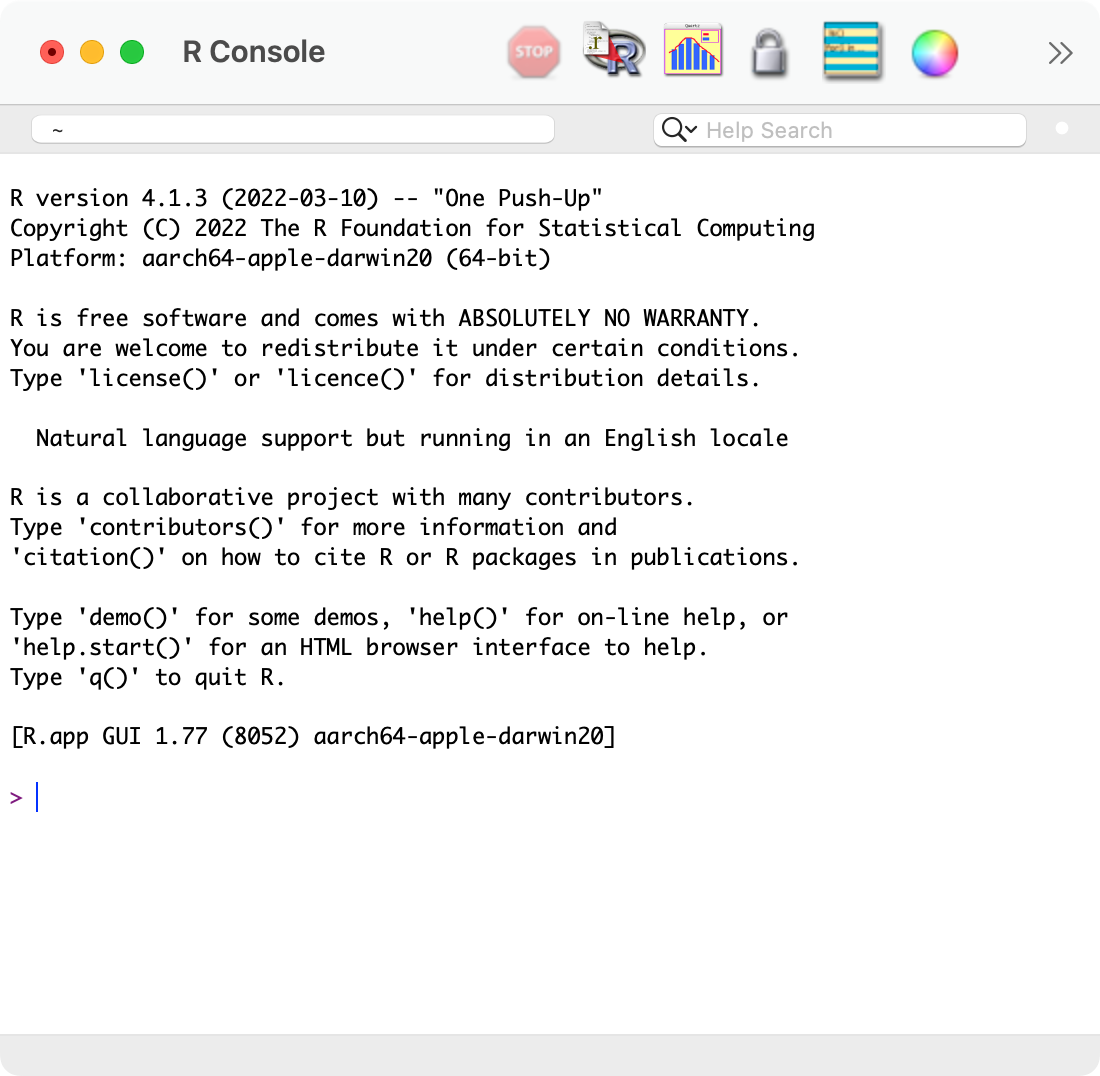
\includegraphics[width=0.8\linewidth]{img/R-screenshot}

Near the bottom of the R screen, you will find the ``\textgreater{}'' symbol which represents the command line. If you type \texttt{1\ +\ 2} into the command line and then hit enter you should get:

\texttt{{[}1{]}\ 3}

This is R performing your calculation, with the \texttt{{[}1{]}} indicating that the solution to \texttt{1\ +\ 2} is a single number (the number 3).

At this point, close R - we will not interact with R like this in the future. You can close R by typing \texttt{quit()} at the command prompt, followed by the return key, or in the usual way of closing an application in your operating system. There is no need to save anything here if prompted.

\hypertarget{to-install-rstudio-on-your-computer}{%
\subsection{To install RStudio on your computer}\label{to-install-rstudio-on-your-computer}}

\begin{enumerate}
\def\labelenumi{\arabic{enumi}.}
\tightlist
\item
  Make sure you have already installed R, and verified that it is working.
\item
  Download the RStudio desktop installer at: \url{https://www.rstudio.com/products/rstudio/download}. Ensure that you select the RStudio Desktop (Free) installer in the first column.
\item
  Install RStudio by running the installer and following the installation instructions. The default settings are fine.
\item
  Open RStudio, which will appear as below:
\end{enumerate}

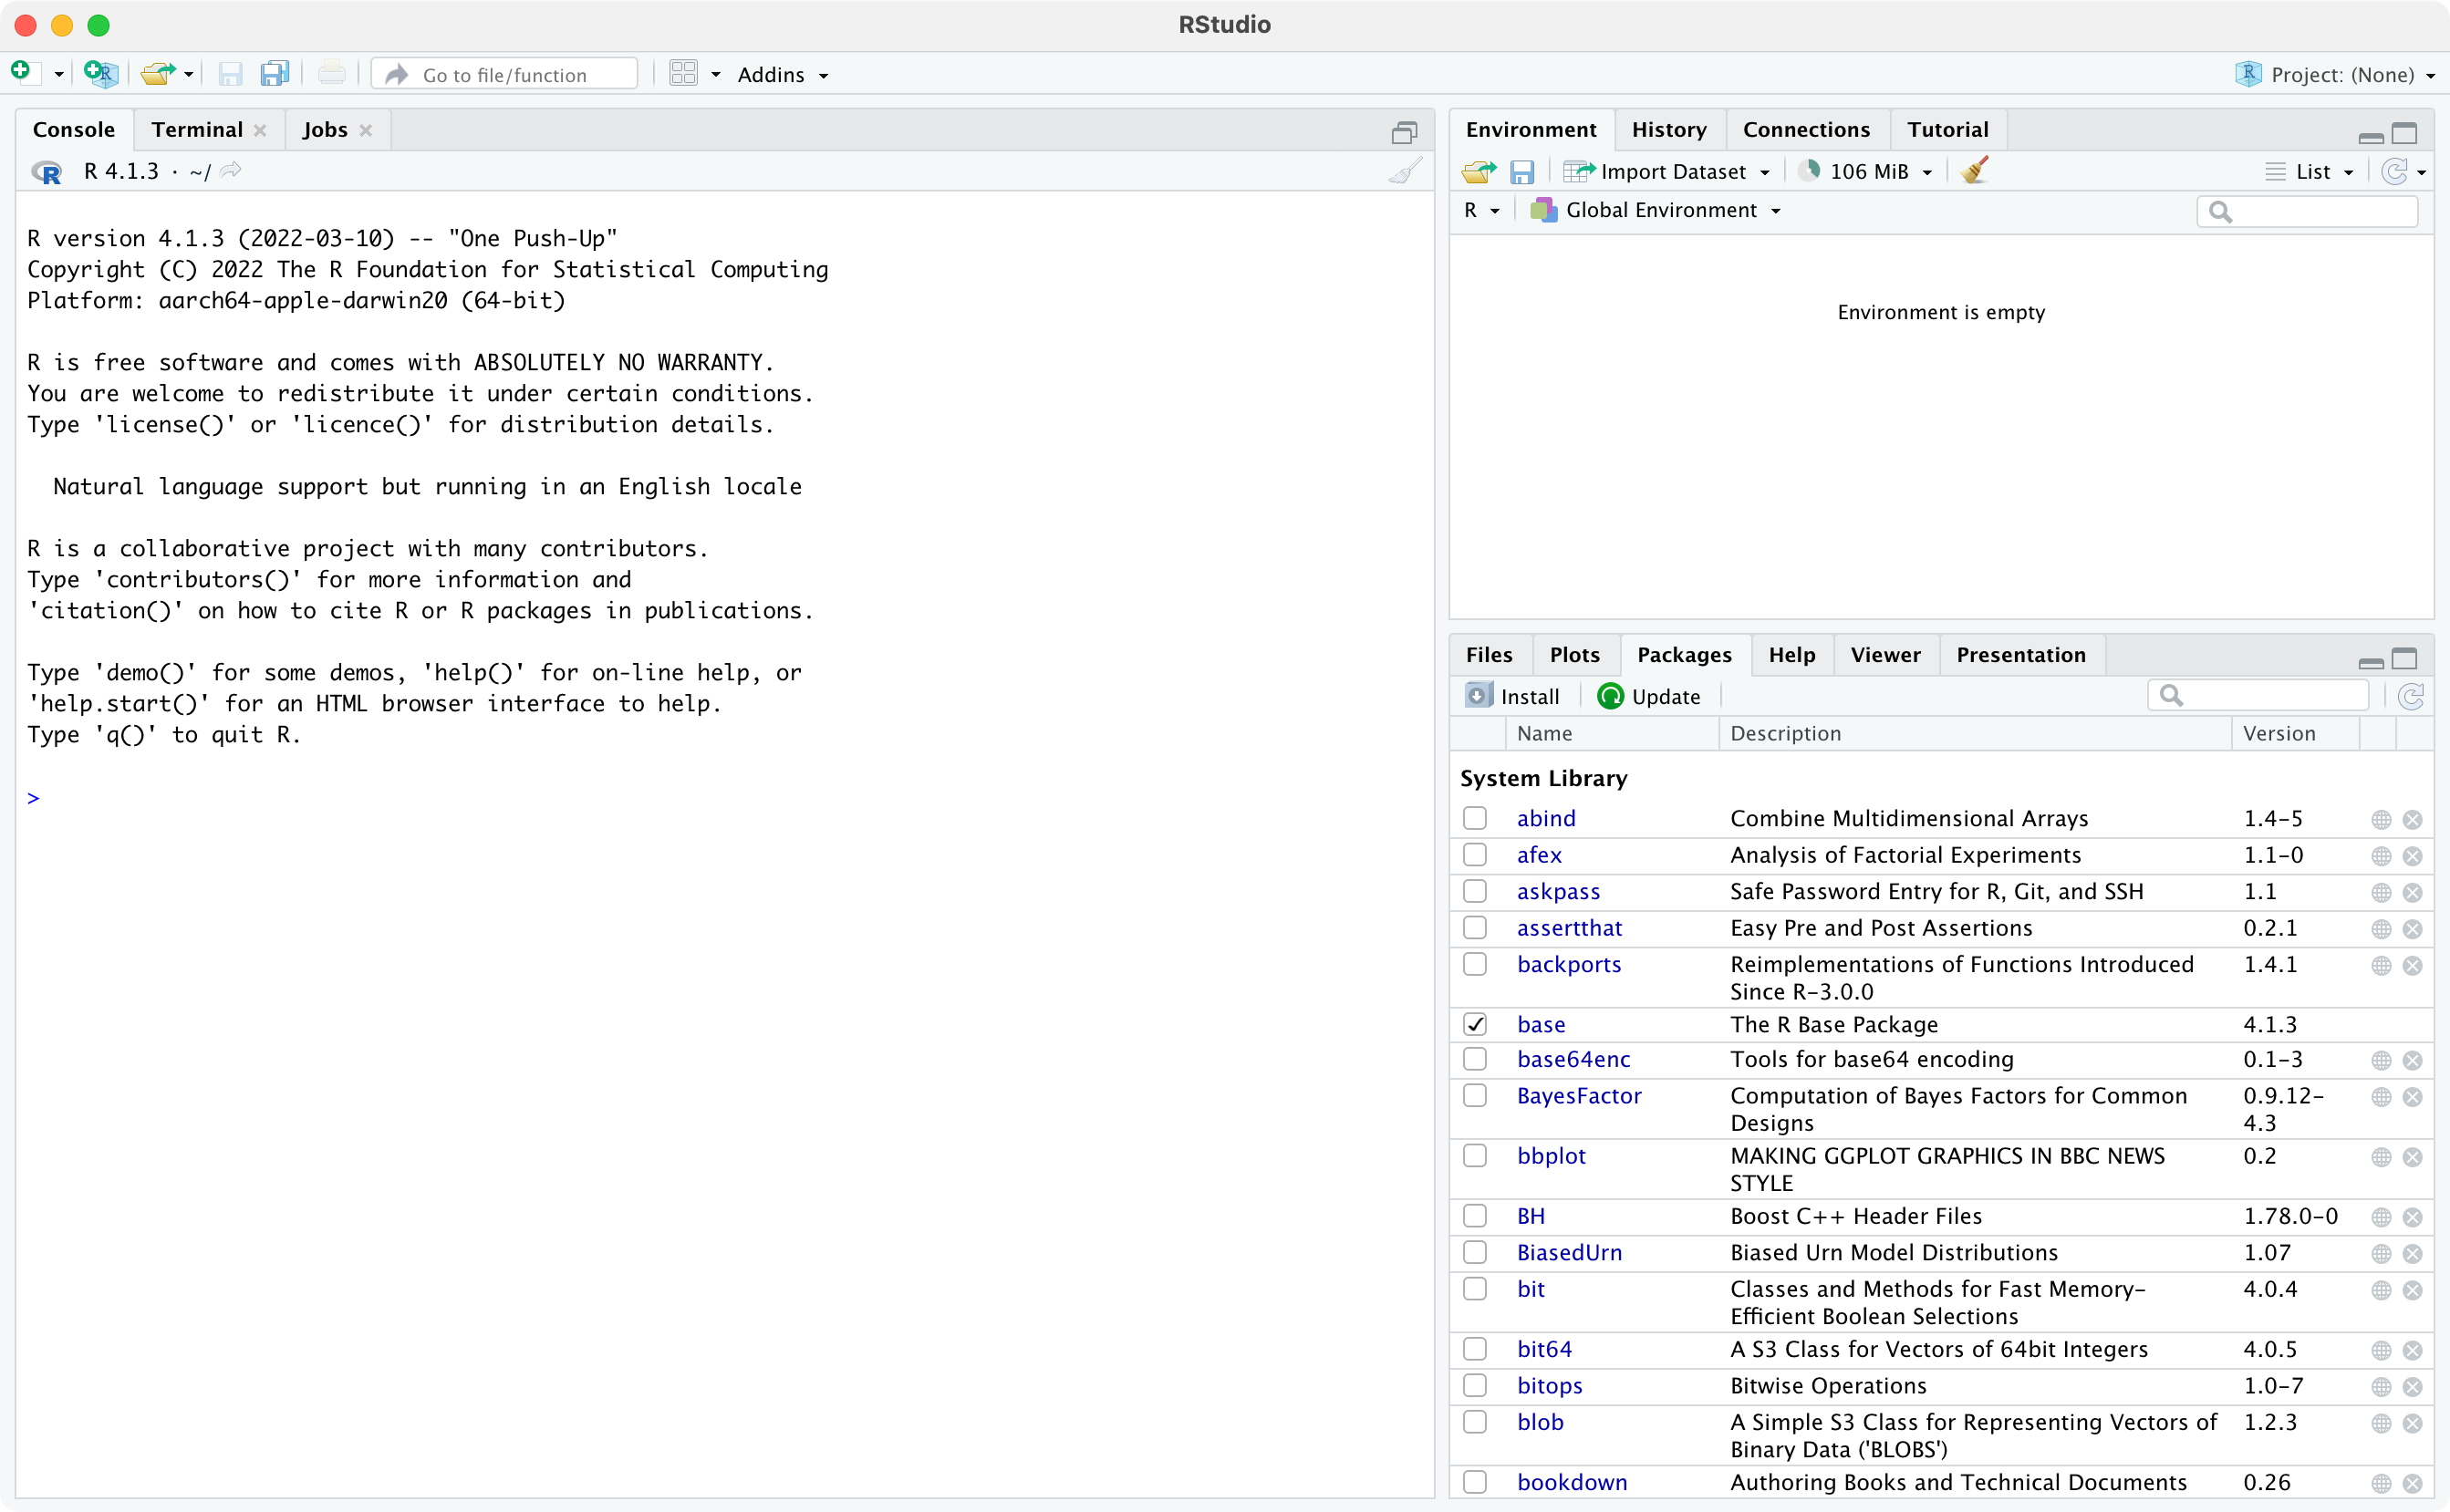
\includegraphics[width=1\linewidth]{img/RStudio-screenshot-01}

Locate the command line symbol ``\textgreater{}'' at the bottom of the left-hand panel. Type \texttt{1\ +\ 2} into the command line and hit enter, and you will see:

\texttt{{[}1{]}\ 3}

This confirms that RStudio is running correctly, and can use the R language to correctly calculate the sum between 1 and 2!

RStudio currently comprises three window panes, and we will discuss these later.

\hypertarget{recommended-setup}{%
\section{Recommended setup}\label{recommended-setup}}

I will provide a recommended setup for R and RStudio in this section. You are free to use alternative workflows and setup, but this setup works well in practice.

\hypertarget{rstudio-preferences}{%
\subsection{RStudio preferences}\label{rstudio-preferences}}

By default, RStudio will retain data, scripts and other objects when you quit your RStudio session. Relying on this can cause headaches, so I recommend that you set up RStudio so that it does not preserve your workspace between sessions. Open the RStudio options:

\begin{itemize}
\item
  Mac: \textbf{RStudio \textgreater{} Preferences}
\item
  Windows: \textbf{Tools \textgreater{} Options}
\end{itemize}

and \textbf{deselect ``Restore .RData into workplace at startup''}, and choose: ``\textbf{Save workspace to .RData on exit:} \textbf{Never''}.

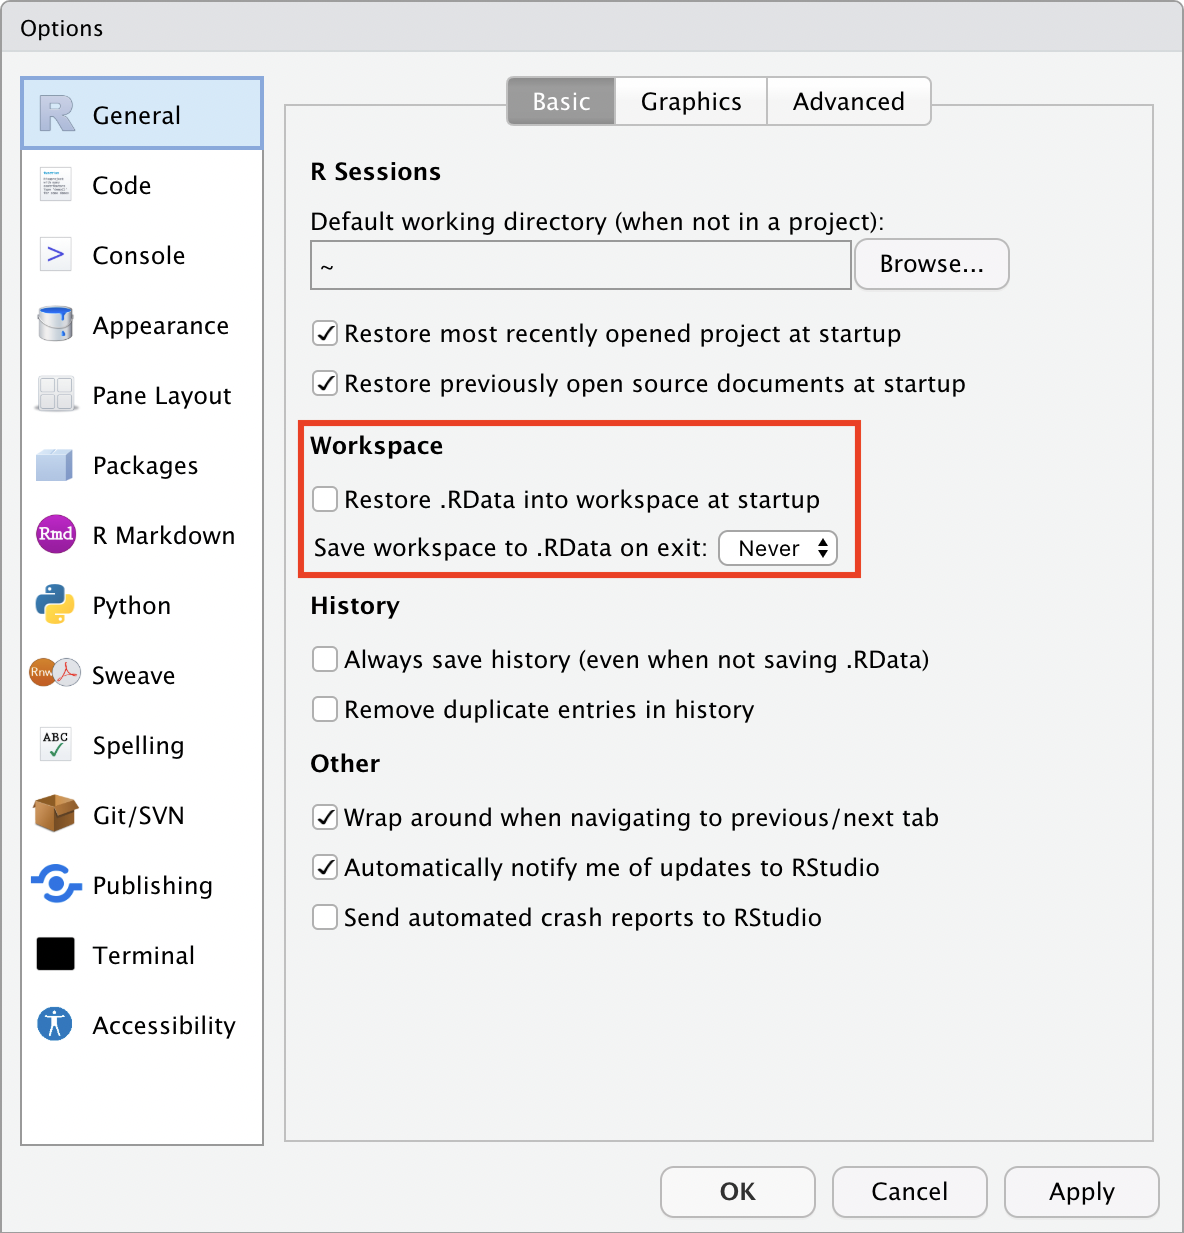
\includegraphics[width=0.75\linewidth]{img/RStudio-preferences}

\hypertarget{set-up-a-project}{%
\subsection{Set up a project}\label{set-up-a-project}}

A project in RStudio is a folder that RStudio recognises as a place to store R scripts, data files, figures that are common to an analysis project. Setting up a folder allows much more simple navigation and specification of data files and output. More detail can be found in Chapter 8 of the excellent text: \href{https://r4ds.had.co.nz/workflow-projects.html}{R for Data Science}. Using projects is not necessary, but I recommend working with projects from day one.

We will create a project called \textbf{PHCM9795} to store all the data you will use and scripts that you will write in this course. First, think about where you want to store your project folder: this could be somewhere in your \emph{Documents} folder.

Step 1: Choose \textbf{File \textgreater{} New Project\ldots{}} in RStudio to open the \textbf{Create Project} dialog box:

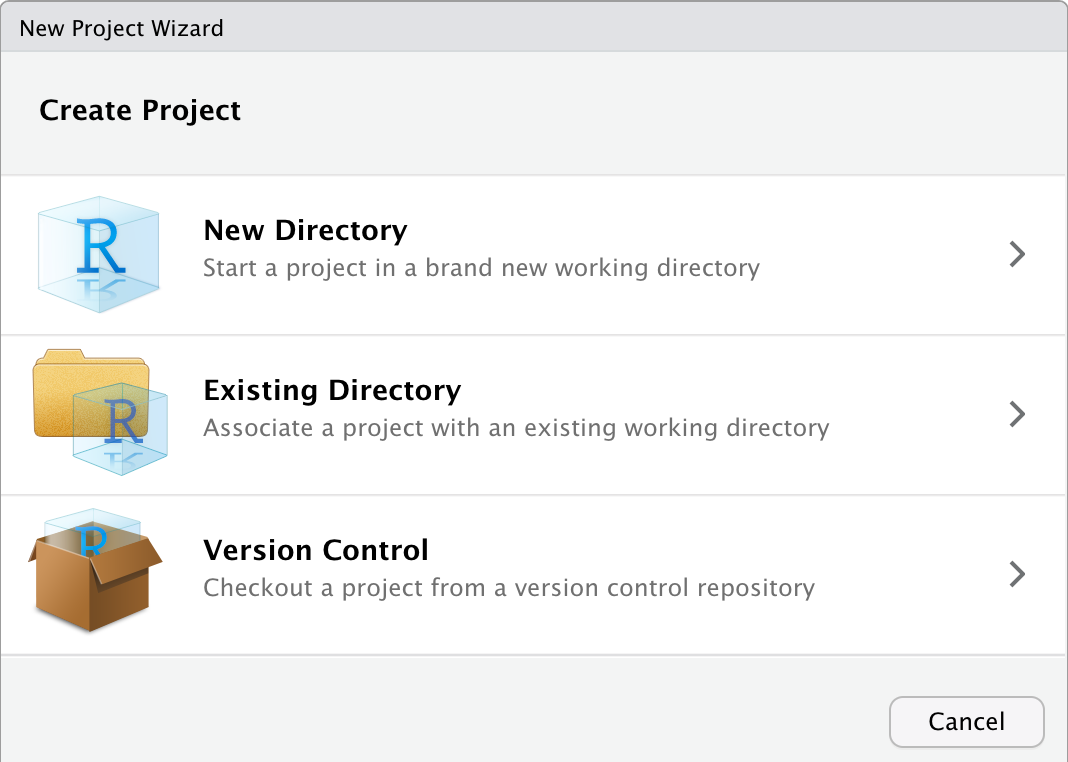
\includegraphics[width=0.75\linewidth]{img/NewProject-1}

Step 2: Click the first option to create a project in a \textbf{New directory}

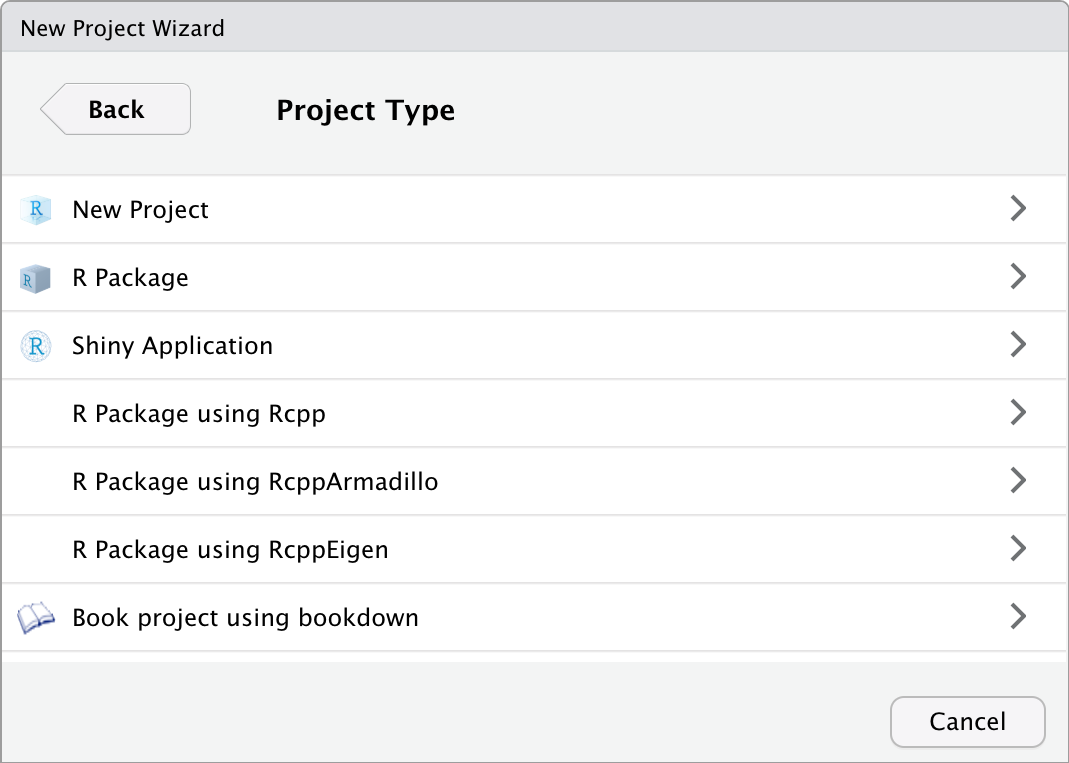
\includegraphics[width=0.75\linewidth]{img/NewProject-2}

Step 3: Click the first option: \textbf{New Project}. Give the project a name, by typing PHCM9795 in the ``Directory name'', and choose where you want to store the project by clicking the \textbf{Browse} button.

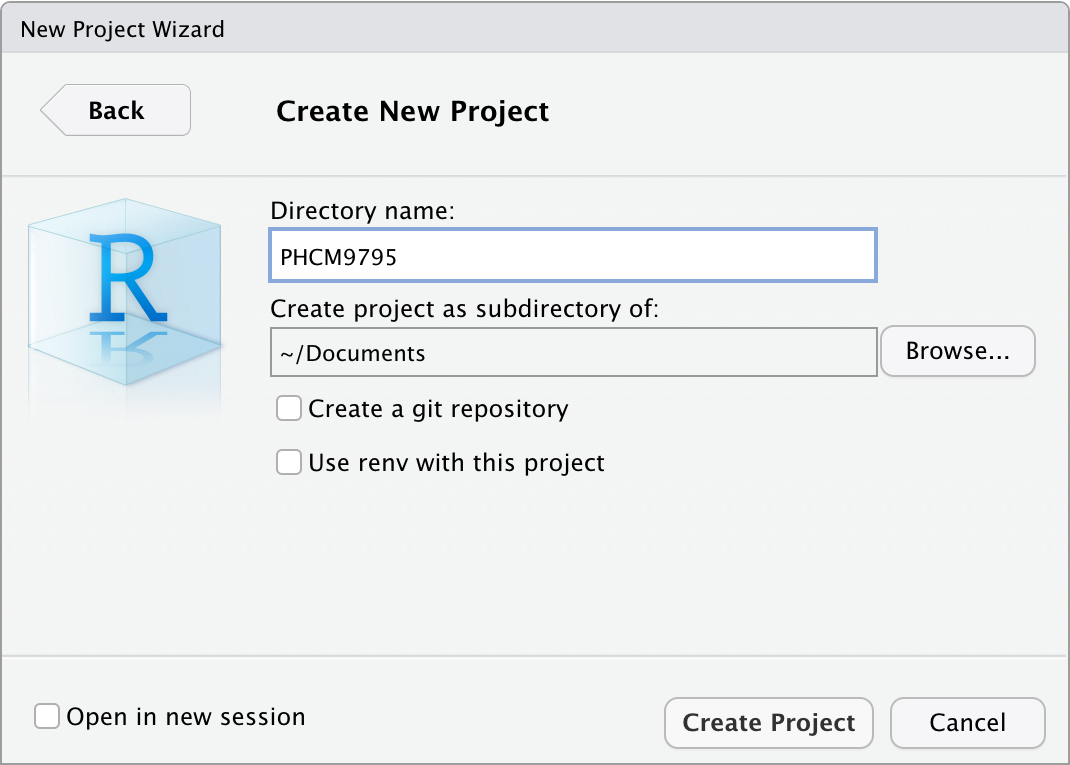
\includegraphics[width=0.75\linewidth]{img/NewProject-3}

Step 4: Click \textbf{Create} to create your project.

You will now have a new folder in your directory, which contains only one file: PHCM9795.Rproj, and the two right-hand panes of RStudio will appear as below:

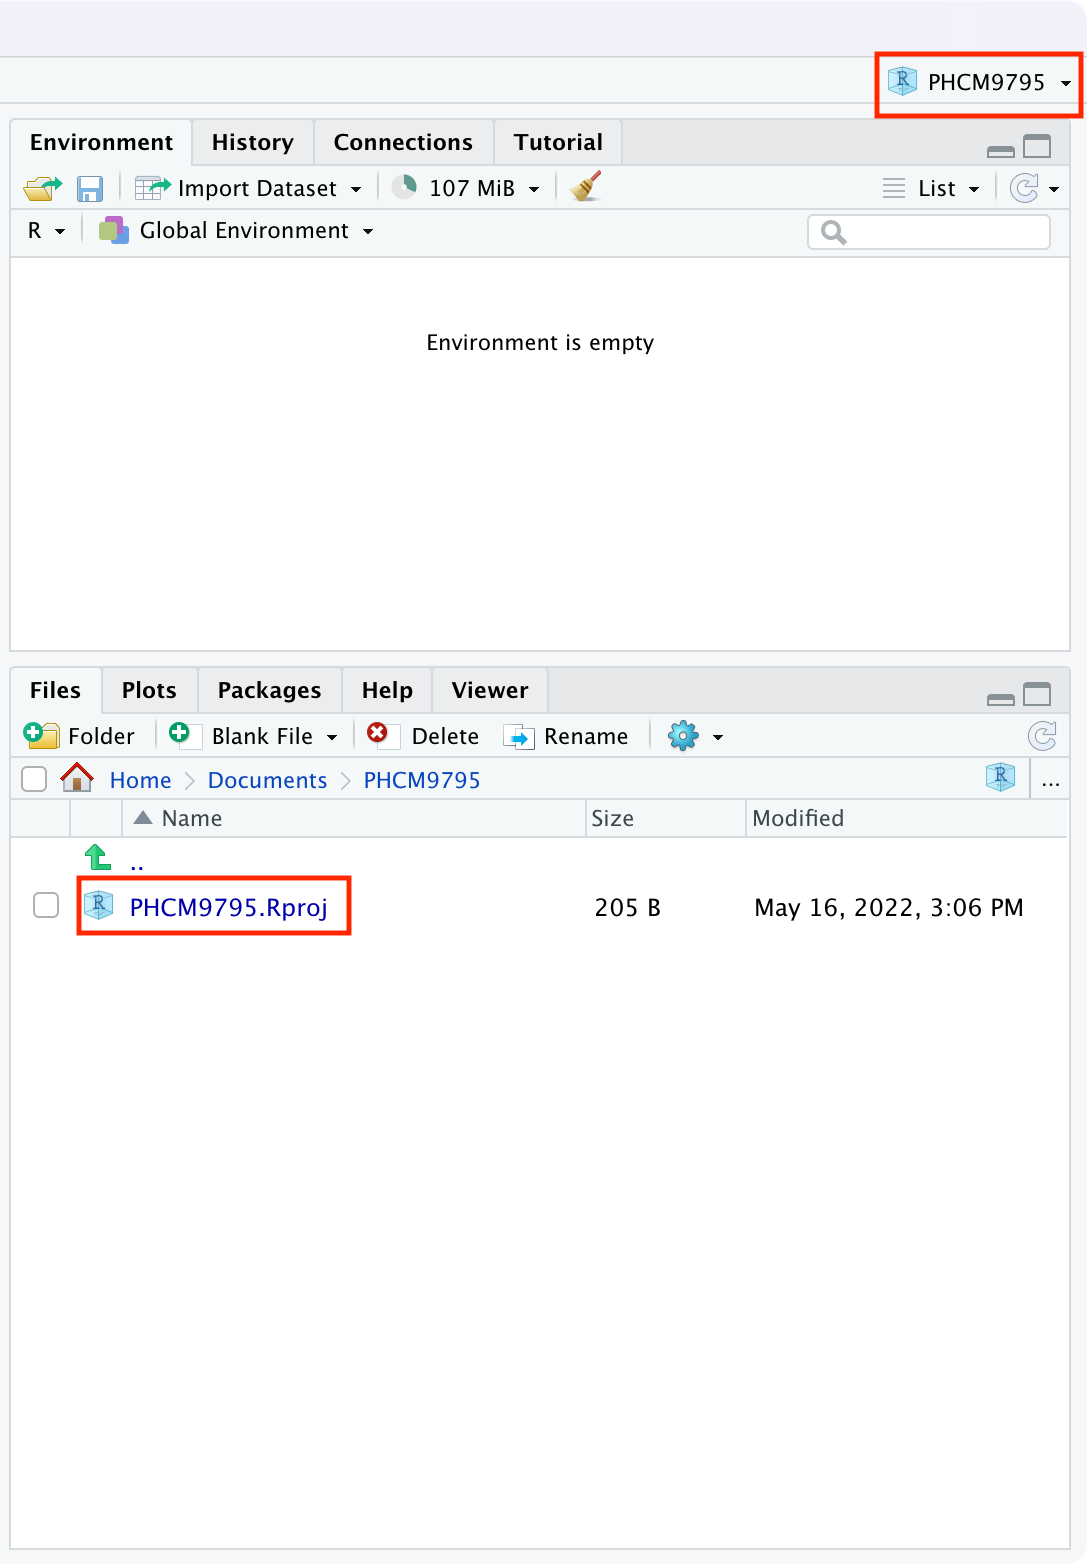
\includegraphics[width=0.75\linewidth]{img/NewProject-4}

The top-right menu bar is showing that you are working within the PHCM9795 project, and the bottom-right window is showing the contents of that window: the single PHCM9795.Rproj file. We will add some more files to this project later.

\hypertarget{simpleR}{%
\section{A simple R analysis}\label{simpleR}}

In this very brief section, we will introduce R by calculating the average of six ages.

To begin, open a new R Script by choosing \textbf{File \textgreater{} New file \textgreater{} R Script} . A script (or a program) is a collection of commands that are sequentially processed by R. You can also type Ctrl+Shift+N in Windows, or Command+Shift+N in MacOS to open a new script in RStudio, or click the \textbf{New File} button at the top of the RStudio window.

You should now see four window panes, as below. In the top-left window, type the following (replacing my name with yours, and including today's date):

\begin{Shaded}
\begin{Highlighting}[]
\CommentTok{\# Author: Timothy Dobbins}
\CommentTok{\# Date: 5 April 2022}
\CommentTok{\# Purpose: My first R script}

\NormalTok{age }\OtherTok{\textless{}{-}} \FunctionTok{c}\NormalTok{(}\DecValTok{20}\NormalTok{, }\DecValTok{25}\NormalTok{, }\DecValTok{23}\NormalTok{, }\DecValTok{29}\NormalTok{, }\DecValTok{21}\NormalTok{, }\DecValTok{27}\NormalTok{)}
\FunctionTok{summary}\NormalTok{(age)}
\end{Highlighting}
\end{Shaded}

\textbf{Note: R is case-sensitive}, so you should enter the text exactly as written in these notes.

Your screen should look something like:

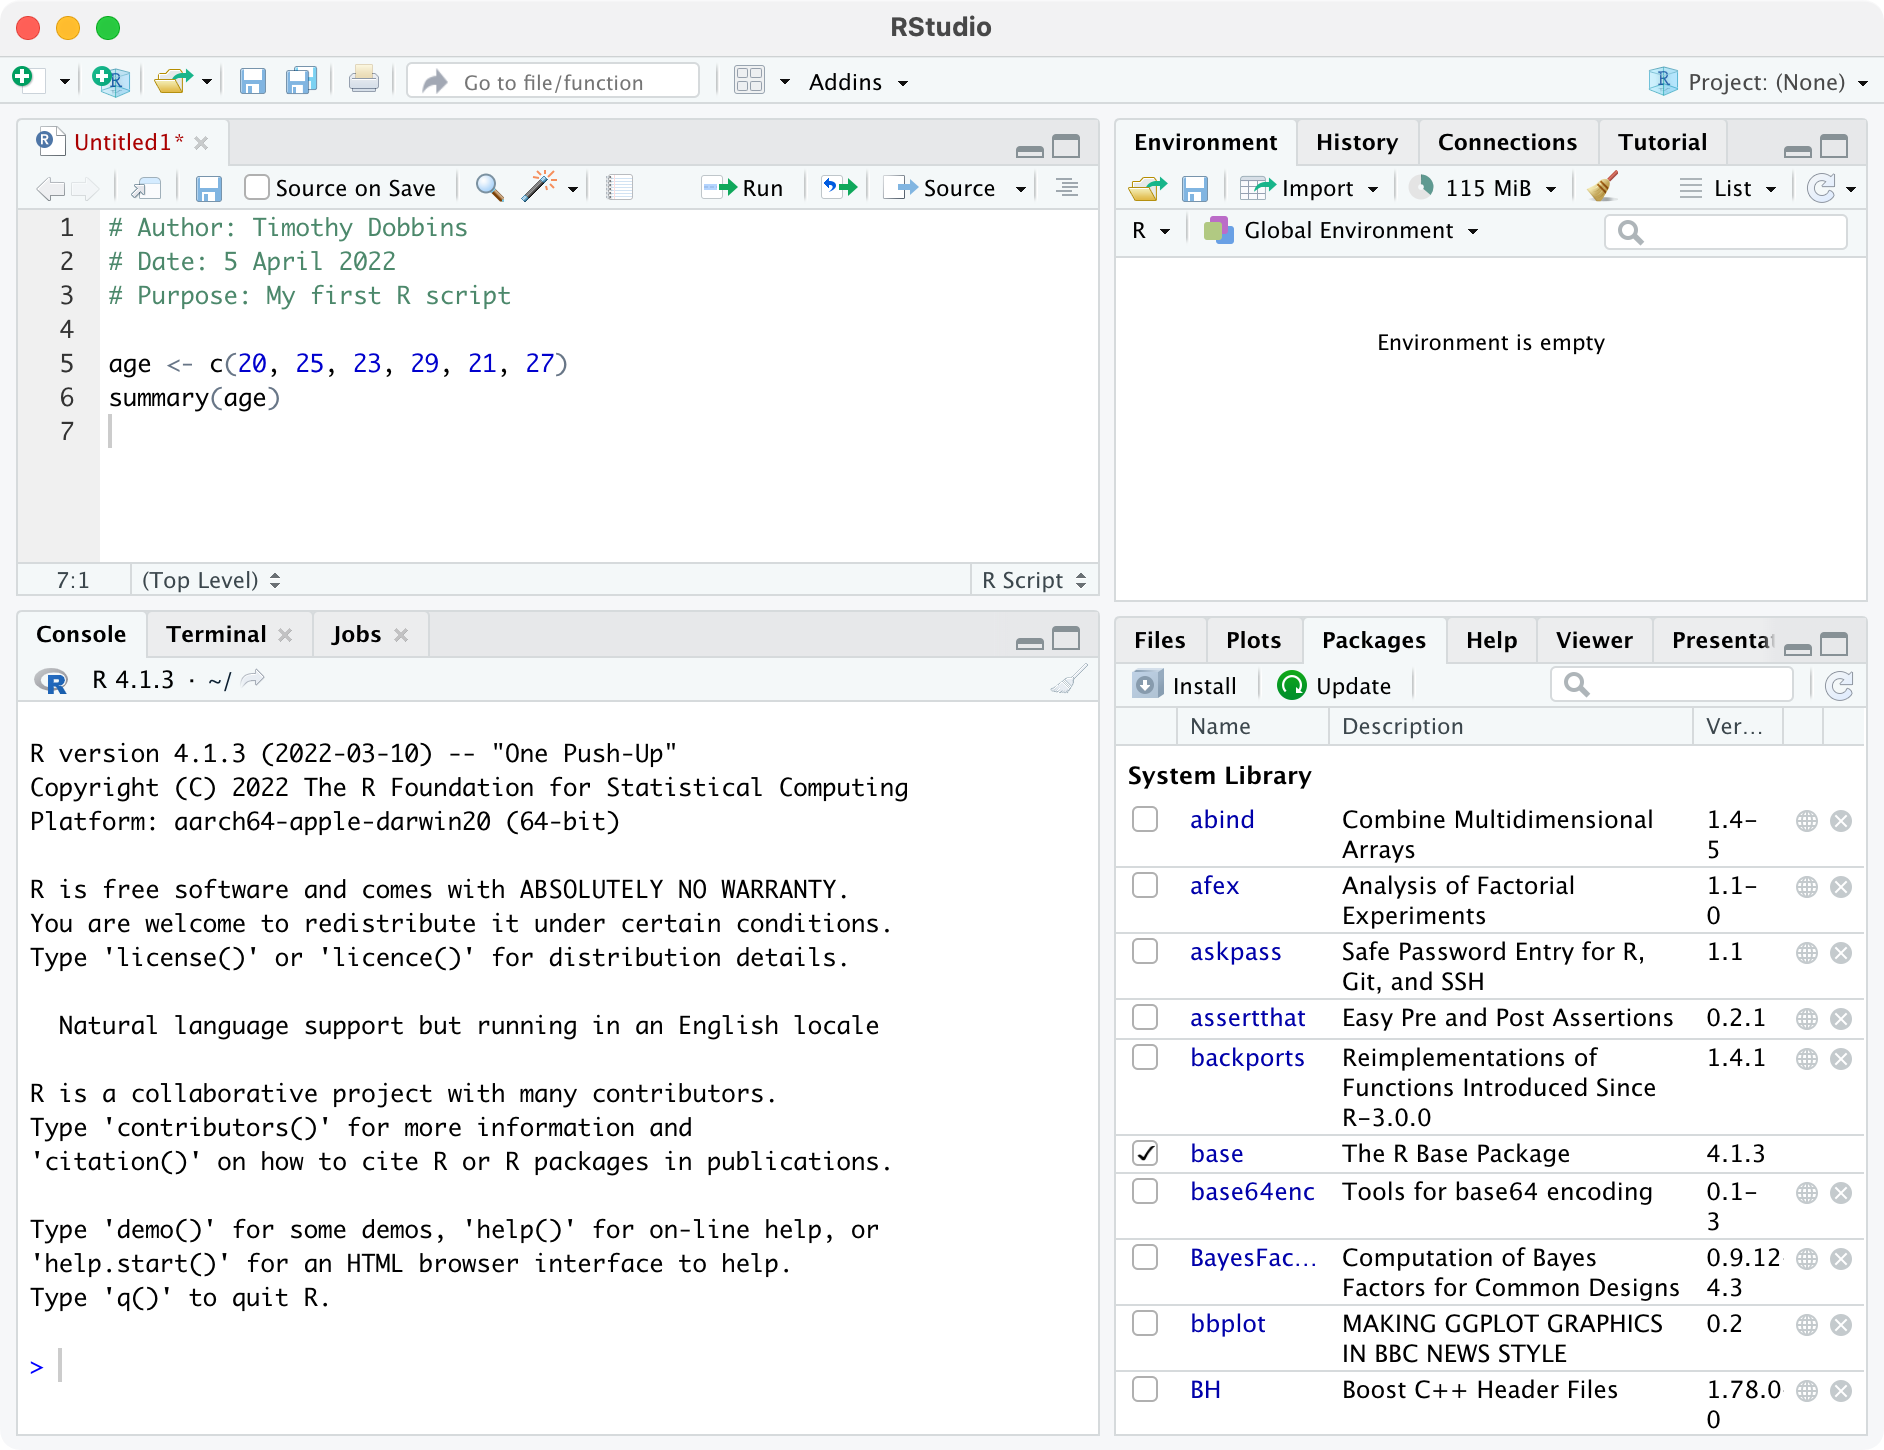
\includegraphics[width=1\linewidth]{img/RStudio-screenshot-02}

To run your script, choose \textbf{Code \textgreater{} Run Region \textgreater{} Run All}. You will see your code appear in the bottom-left window, with the following output:

\begin{Shaded}
\begin{Highlighting}[]
\SpecialCharTok{\textgreater{}} \CommentTok{\# Author: Timothy Dobbins}
\ErrorTok{\textgreater{}} \CommentTok{\# Date: 5 April 2022}
\ErrorTok{\textgreater{}} \CommentTok{\# Purpose: My first R script}
\ErrorTok{\textgreater{}} 
\ErrorTok{\textgreater{}}\NormalTok{ age }\OtherTok{\textless{}{-}} \FunctionTok{c}\NormalTok{(}\DecValTok{20}\NormalTok{, }\DecValTok{25}\NormalTok{, }\DecValTok{23}\NormalTok{, }\DecValTok{29}\NormalTok{, }\DecValTok{21}\NormalTok{, }\DecValTok{27}\NormalTok{)}

\SpecialCharTok{\textgreater{}} \FunctionTok{summary}\NormalTok{(age)}
\NormalTok{   Min. 1st Qu.  Median    Mean 3rd Qu.    Max. }
  \FloatTok{20.00}   \FloatTok{21.50}   \FloatTok{24.00}   \FloatTok{24.17}   \FloatTok{26.50}   \FloatTok{29.00} 
\end{Highlighting}
\end{Shaded}

We will explain the key parts of this script later, but for now, you have entered six ages and calculated the mean age (along with five other summary statistics).

Save your script within the PHCM9795 project by using \textbf{File \textgreater{} Save As}, using the name \texttt{my\_first\_analysis.R}.

\hypertarget{the-rstudio-environment}{%
\section{The RStudio environment}\label{the-rstudio-environment}}

Now that we have seen a simple example of how to use R within RStudio, let's describe the RStudio environment. Let's assume that you have just run your first R script, and you have four windows as below:

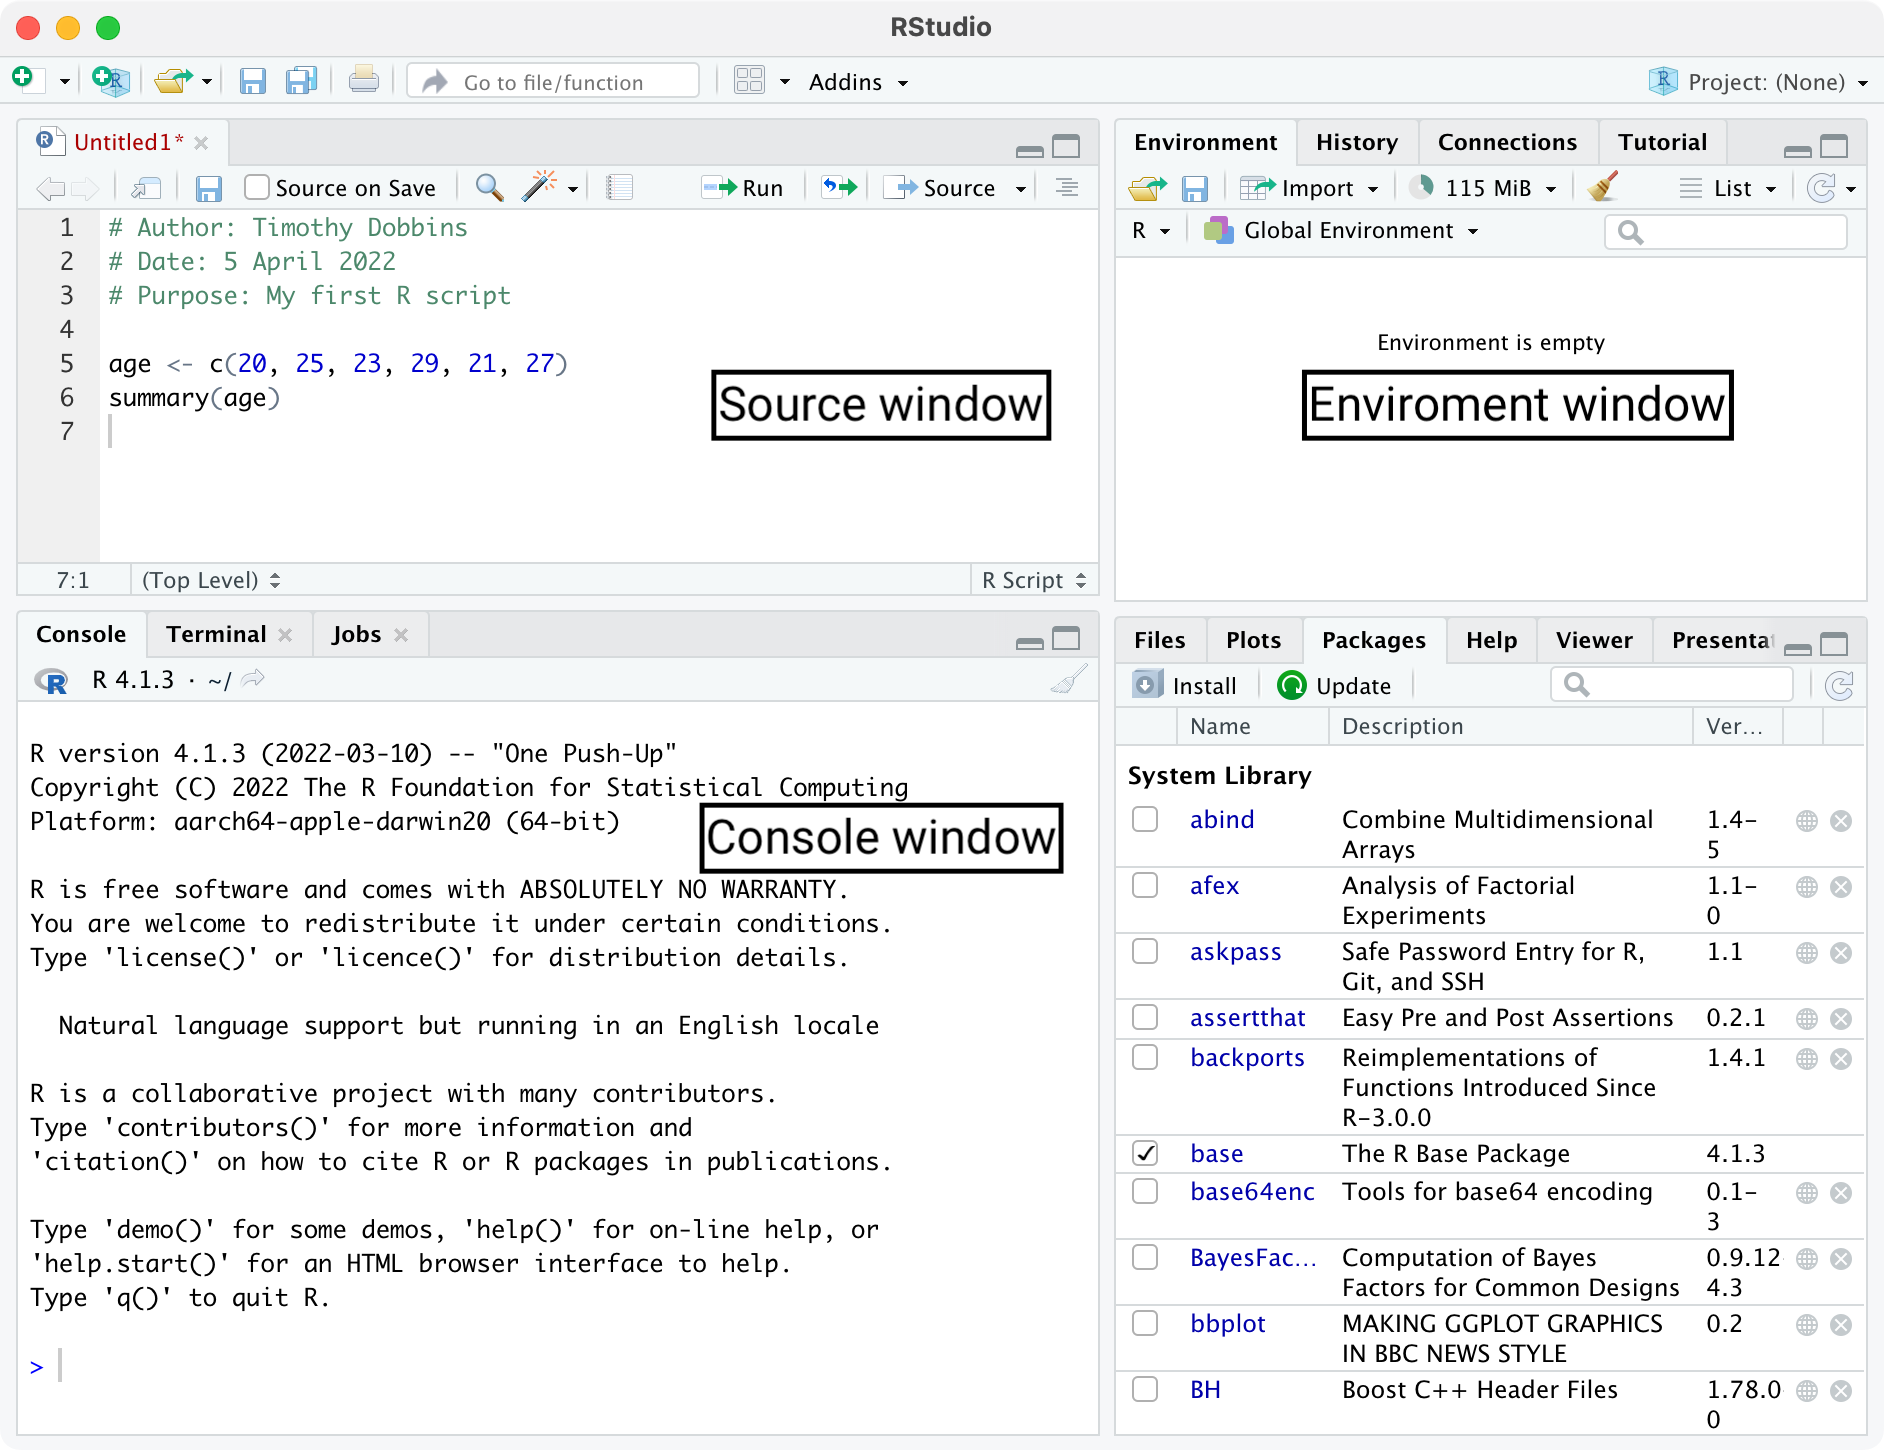
\includegraphics[width=1\linewidth]{img/RStudio-screenshot-03}

The top-left window is call the \textbf{Source} window, and is where you write and edit your R scripts. Scripts can be saved by clicking \textbf{File \textgreater{} Save As} or by clicking on the symbol of a floppy disk at the top of the script. The file will have an extension of .R, for example script.R. Remember to give your script a meaningful title and remember to periodically save as you go.

In RStudio, the name of the script will be black when it has been saved, and will change to red if you have any unsaved changes.

The \textbf{Console} window, at the bottom left, contains the command line which is indicated with the symbol \textgreater. You can type commands here, but anything executed directly from the console is not saved and therefore is lost when the session ends (when you exit RStudio). You should always run your commands from a script file which you can save and use again later. When you run commands from a script, the output and any notes/errors are shown in the console. The Terminal and Jobs tabs will not be used in this course.

The \textbf{Environment} window at the top-right shows a list of objects that have been created during your session. When you close your RStudio session these objects will disappear. We will not use the History or Connections tabs in this course.

The bottom right corner contains some useful tabs, in particular the \textbf{Help} tab. When you are troubleshooting errors or learning how to use a function, the Help tab should be the first place you visit. Here you can search the help documents for all the packages you have installed. Whenever you create plots in R, these will be shown in the \textbf{Plots} tab. The \textbf{Packages} tab contains a list of installed packages and indicates which ones are currently in use (we will learn about packages later). Packages which are loaded, i.e.~in use, are indicated with a tick. Some packages are in use by default when you begin a new session. You can access information about a package by clicking on its name. The \textbf{Files} tab provides a shortcut to access your files. The Viewer tab will not be used in this course.

\hypertarget{some-r-basics}{%
\section{Some R basics}\label{some-r-basics}}

While we use R as a statistics package, R is a programming language. In order to use R effectively, we need to define some basics.

\hypertarget{scripts}{%
\subsection{Scripts}\label{scripts}}

While R can be run completely from the command line, issuing commands one-by-one, it is most commonly run using \textbf{scripts}. A script is simply a list of commands that are processed in order. The simple analysis we conducted earlier is a very simple script. Some things to know about R scripts:

\begin{itemize}
\item
  anything appearing after a \# is a comment, and is ignored by R. The first three lines of our script are there for ourselves (either as writers of code, or readers of code). I include comments at the beginning of each of my scripts to describe:

  \begin{itemize}
  \item
    who wrote the script (useful if someone else uses your script and wants to ask questions about it);
  \item
    when the script was written;
  \item
    what the script does. This last point may seem odd, but it's useful to describe what this script does, and why it might differ to other scripts being used in the analysis. This is particularly useful if your scripts become long and complex.
  \end{itemize}
\item
  \textbf{R is case-sensitive}. So \texttt{age}, \texttt{AGE} and \texttt{Age} could refer to three separate variables (please don't do this!)
\item
  use blank lines and comments to separate sections of your script
\end{itemize}

\hypertarget{objects}{%
\subsection{Objects}\label{objects}}

If you do some reading about R, you may learn that R is an ``object-oriented programming language''. When we enter or import data into R, we are asking R to create \textbf{objects} from our data. These objects can be manipulated and transformed by \textbf{functions}, to obtain useful insights from our data.

Objects in R are created using the \textbf{assignment operator}. The most common form of the assignment operator looks like an arrow: \texttt{\textless{}-} and is typed as the \texttt{\textless{}} and \texttt{-} symbols. The simplest way of reading \texttt{\textless{}-} is as the words ``is defined as''. Note that it possible to use \texttt{-\textgreater{}} and even \texttt{=} as assignment operators, but their use is less frequent.

Let's see an example:

\begin{Shaded}
\begin{Highlighting}[]
\NormalTok{x }\OtherTok{\textless{}{-}} \DecValTok{42}
\end{Highlighting}
\end{Shaded}

This command creates a new object called \texttt{x}, which is defined as the number 42 (or in words, ``\texttt{x} is defined as 42''). Running this command gives no output in the console, but the new object appears in the top-right \textbf{Environment} panel. We can view the object in the console by typing its name:

\begin{Shaded}
\begin{Highlighting}[]
\CommentTok{\# Print the object x}
\NormalTok{x}
\end{Highlighting}
\end{Shaded}

\begin{verbatim}
## [1] 42
\end{verbatim}

Now we see the contents of \texttt{x} in the console.

This example is rather trivial, and we rarely assign objects of just one value. In fact, we created an object earlier, called \texttt{age}, which comprised six values.

\hypertarget{data-structures}{%
\subsection{Data structures}\label{data-structures}}

There are two main structures we will use to work with data in this course: \textbf{vectors} and \textbf{data frames}. A \textbf{vector} is a combination of data values, all of the same type. For example, our six ages that we entered earlier is a vector. You could think of a vector as a column of data (even though R prints vectors as rows!) And technically, even an object with only one value is a vector, a vector of size 1.

The easiest way of creating a vector in R is by using the \texttt{c()} function, where c stands for `combine'. In our previous Simple Analysis in R (Section \ref{simpleR}), we wrote the command:

\begin{Shaded}
\begin{Highlighting}[]
\NormalTok{age }\OtherTok{\textless{}{-}} \FunctionTok{c}\NormalTok{(}\DecValTok{20}\NormalTok{, }\DecValTok{25}\NormalTok{, }\DecValTok{23}\NormalTok{, }\DecValTok{29}\NormalTok{, }\DecValTok{21}\NormalTok{, }\DecValTok{27}\NormalTok{)}
\end{Highlighting}
\end{Shaded}

This command created a new object called \texttt{age}, and \emph{combined} the six values of age into one vector.

Just as having a vector of size 1 is unusual, having just one column of data to analyse is also pretty unusual. The other structure we will describe here is a \textbf{data frame} which is essentially a collection of vectors, each of the same size. You could think of a data frame as being like a spreadsheet, with columns representing variables, and rows representing observations.

There are other structures in R, such as matrices and lists, which we won't discuss in this course. And you may come across the term \textbf{tibble}, which is a type of data frame.

\hypertarget{functions}{%
\subsection{Functions}\label{functions}}

If objects are the nouns of R, functions are the verbs. Essentially, functions transform objects. Functions can transform your data into summary statistics, graphical summaries or analysis results. For example, we used the \texttt{summary()} function to display summary statistics for our six ages.

R functions are specified by their arguments (or inputs). The arguments that can be supplied for each function can be inspected by examining the help notes for that function. To obtain help for a function, we can submit \texttt{help(summary)} (or equivalently \texttt{?summary}) in the console, or we can use the \textbf{Help} tab in the bottom-right window of RStudio. For example, the first part of the help notes for \texttt{summary} appear as:

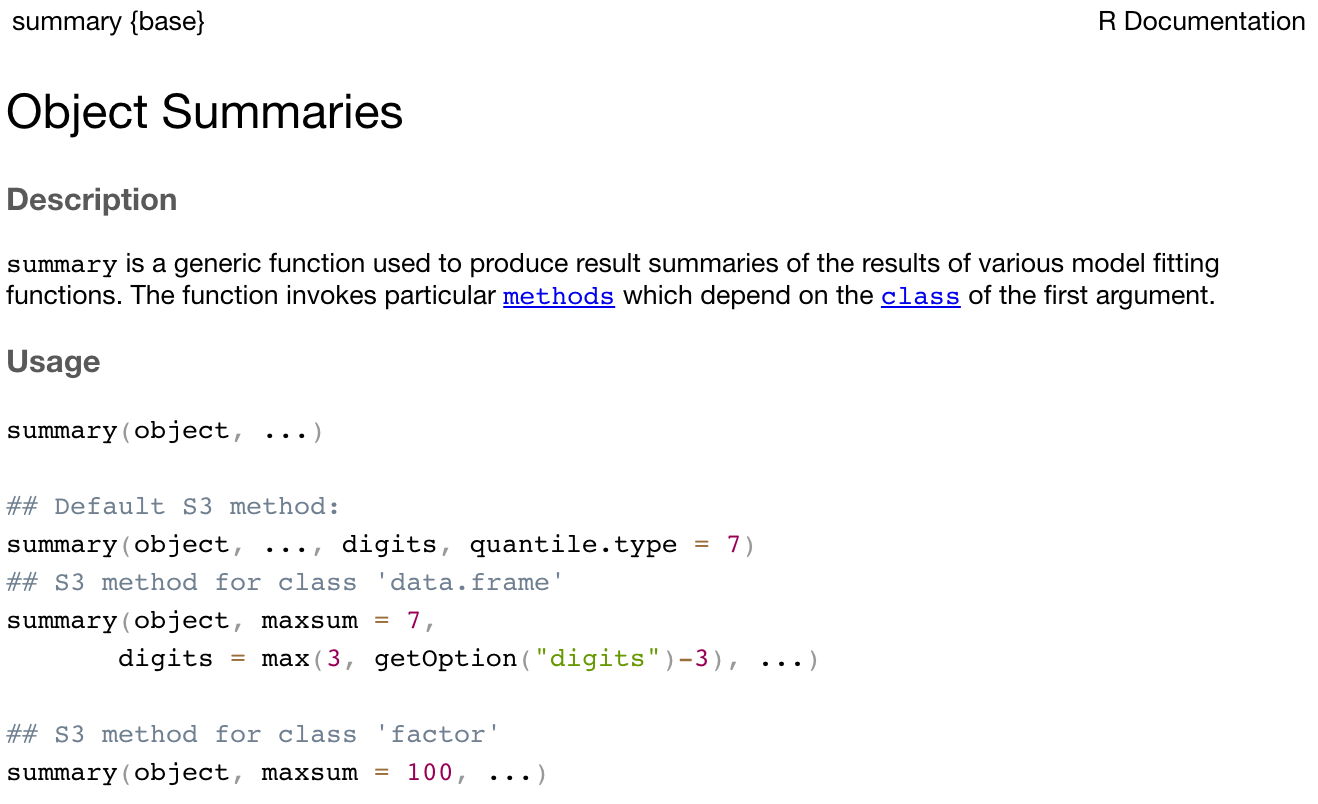
\includegraphics[width=0.8\linewidth]{img/help-1}

The help notes in R can be quite cryptic, but the \textbf{Usage} section details what inputs should be specified for the function to run. Here, \texttt{summary} requires an object to be specified. In our case, we specified \texttt{age}, which is our object defined as the vector of six ages.

Most help pages also include some examples of how you might use the function. These can be found at the very bottom of the help page.

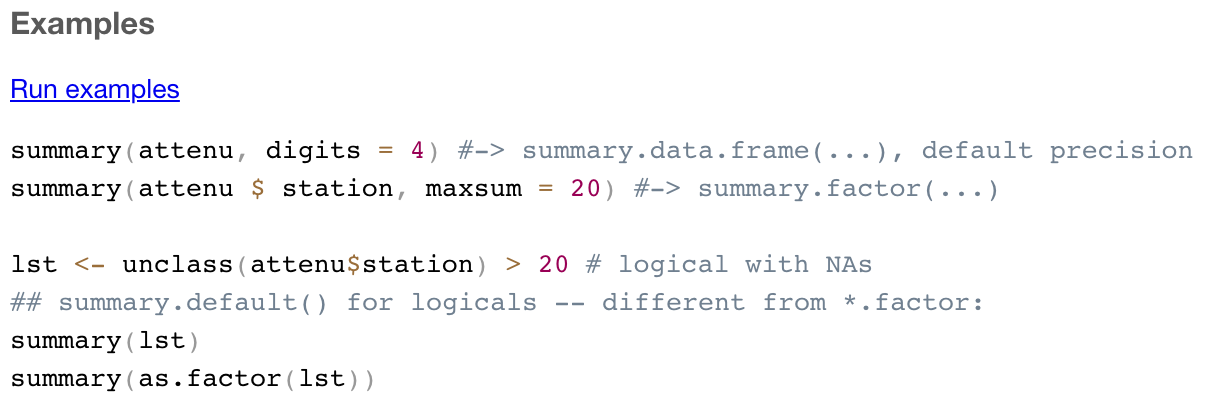
\includegraphics[width=0.8\linewidth]{img/help-2}

The \texttt{summary()} function is quite simple, in that it only requires one input, the object to be summarised. More complex functions might require a number of inputs. For example, the help notes for the \texttt{descriptives()} function in the \texttt{jmv} package show a large number of inputs can be specified:

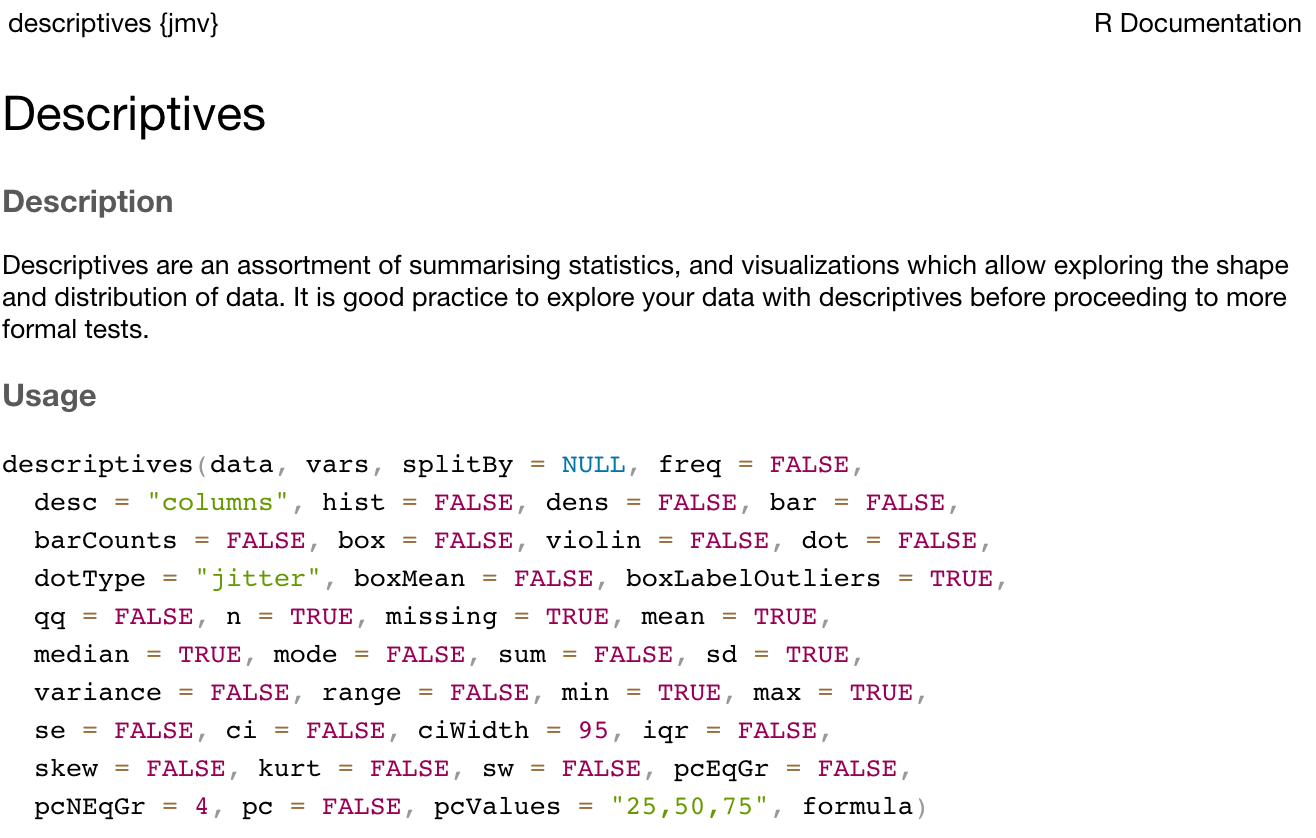
\includegraphics[width=0.8\linewidth]{img/help-3}

There are two things to note here. First, notice that the first two inputs are listed with no = symbol, but all other inputs are listed with = symbols (with values provided after the = symbol). This means that everything apart from \texttt{data} and \texttt{vars} have \textbf{default} values. We are free to not specify values for these inputs if we are happy with the defaults provided. For example, by default the variance is not calculated (as \texttt{variance\ =\ FALSE}). To obtain the variance as well as the standard deviation, we can change this default to \texttt{variance\ =\ TRUE}:

\begin{Shaded}
\begin{Highlighting}[]
\CommentTok{\# Only the standard deviation is provided as the measure of variability}
\FunctionTok{descriptives}\NormalTok{(}\AttributeTok{data=}\NormalTok{pbc, }\AttributeTok{vars=}\NormalTok{age)}

\CommentTok{\# Additionally request the variance to be calculated}
\FunctionTok{descriptives}\NormalTok{(}\AttributeTok{data=}\NormalTok{pbc, }\AttributeTok{vars=}\NormalTok{age, }\AttributeTok{variance=}\ConstantTok{TRUE}\NormalTok{)}
\end{Highlighting}
\end{Shaded}

Second, for functions with multiple inputs, we can specify the input name and its value, or we can ignore the input name and specify just the input values \textbf{in the order listed in the Usage section}. So the following are equivalent:

\begin{Shaded}
\begin{Highlighting}[]
\CommentTok{\# We can specify that the dataset to be summarised is pbc,}
\CommentTok{\#   and the variable to summarise is age:}
\FunctionTok{descriptives}\NormalTok{(}\AttributeTok{data=}\NormalTok{pbc, }\AttributeTok{vars=}\NormalTok{age)}

\CommentTok{\# We can omit the input name, as long as we keep the inputs in the correct order {-} }
\CommentTok{\#   that is, dataset first, variable second:}
\FunctionTok{descriptives}\NormalTok{(pbc, age)}

\CommentTok{\# We can change the order of the inputs, as long as we specify the input name:}
\FunctionTok{descriptives}\NormalTok{(}\AttributeTok{vars=}\NormalTok{age, }\AttributeTok{data=}\NormalTok{pbc)}
\end{Highlighting}
\end{Shaded}

In this course, we will usually provide all the input names, even when they are not required. As you become more familiar with R, you will start to use the shortcut method.

\hypertarget{the-curse-of-inconsistency}{%
\subsubsection{The curse of inconsistency}\label{the-curse-of-inconsistency}}

As R is an open-source project, many people have contributed to its development. This has led to a frustrating part of R: some functions require a single object to be specified, but some require you to specify a data frame and select variables for analysis. Let's see an example.

The help for \texttt{summary()} specifies the usage as: \texttt{summary(object,\ ...)}. This means we need to specify a single object to be summarised. An object could be a single column of data (i.e.~a vector), or it could be a data frame. If we have a data frame called \texttt{pbc} which contains many variables, the command \texttt{summary(pbc)} would summarise every variable in the data frame.

What if we only wanted to summarise the age of the participants in the data frame? To select a single variable from a data frame, we can use the following syntax: \texttt{dataframe\$variable}. So to summarise just age from this data frame, we would use: \texttt{summary(pbc\$age)}.

Compare this with the \texttt{descriptives()} function in the \texttt{jmv} package. We saw earlier that the two required inputs for \texttt{descriptives()} are \texttt{data} (the data frame to be analysed) and \texttt{vars} (the variables to be analysed). So to summarise \texttt{age} from the \texttt{pbc} data frame, we would specify \texttt{descriptives(data=pbc,\ vars=age)}.

This inconsistency will seem maddening at first, and will continue to be maddening! Reading the \textbf{usage} section of the help pages is a useful way to determine whether you should specify an object (like \texttt{pbc\$age}) or a data frame and a list of variables.

\hypertarget{packages}{%
\subsection{Packages}\label{packages}}

A \textbf{package} is a collection of functions, documentation (and sometimes datasets) that extend the capabilities of R. Packages have been written by R users to be freely distributed and used by others. R packages can be obtained from many sources, but the most common source is CRAN: the Comprehensive R Archive Network.

A useful way of thinking about R is that R is like a smartphone, with packages being like apps which are downloaded from CRAN (similar to an app-store). When you first install R, it comes with a basic set of packages (apps) installed. You can do a lot of things with these basic packages, but sometimes you might want to do things differently, or you may want to perform some analyses that can't be done using the default packages. In these cases, you can install a package.

Like installing an app on a smartphone, you only need to \emph{install} a package once. But each time you want to use the package, you need to \emph{load} the package into R.

\hypertarget{how-to-install-a-package}{%
\subsection{How to install a package}\label{how-to-install-a-package}}

There are a couple of ways to install a package. You can use the \texttt{install.packages()} function if you know the exact name of the package. Let's use an example of installing the \texttt{skimr} package, which gives a very nice, high-level overview of any data frame. We can install \texttt{skimr} by typing the following into the console:

\begin{Shaded}
\begin{Highlighting}[]
\FunctionTok{install.packages}\NormalTok{(}\StringTok{"skimr"}\NormalTok{)}
\end{Highlighting}
\end{Shaded}

Note the use of the quotation marks.

Alternatively, RStudio offers a graphical way of installing packages that can be accessed via \textbf{Tools \textgreater{} Install Packages}, or via the \textbf{Install} button at the top of the \textbf{Packages} tab in the bottom-right window. You can begin typing the name of the package in the dialog box that appears, and RStudio will use predictive text to offer possible packages:

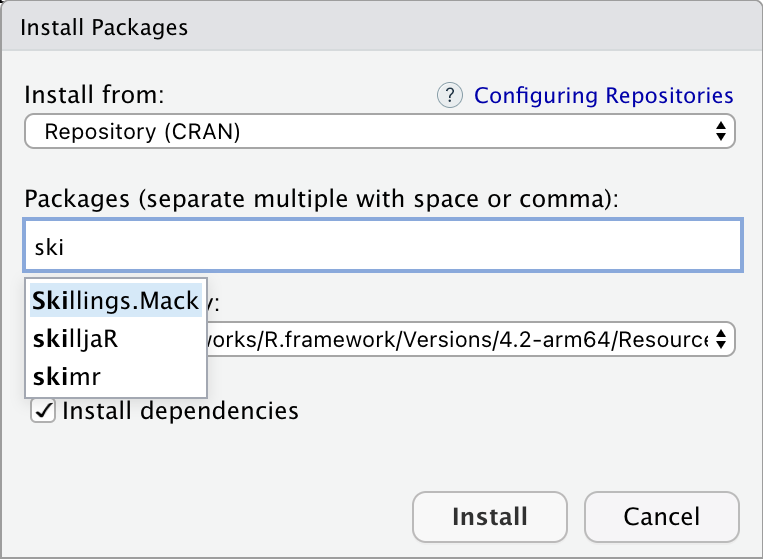
\includegraphics[width=0.6\linewidth]{img/install-packages}

While writing code is usually the recommended way to use R, installing packages is an exception. Using \textbf{Tools \textgreater{} Install Packages} is perfectly fine, because you only need to install a package once.

\hypertarget{how-to-load-a-package}{%
\subsection{How to load a package}\label{how-to-load-a-package}}

When you begin a new session in RStudio, i.e.~when you open RStudio, only certain core packages are automatically loaded. You can use the \texttt{library()} function to load a package that you has previously been installed. For example, now that we have installed \texttt{skimr}, we need to load it before we can use it:

\begin{Shaded}
\begin{Highlighting}[]
\FunctionTok{library}\NormalTok{(skimr)}
\end{Highlighting}
\end{Shaded}

Note that quotation marks are not required for the \texttt{library()} function (although they can be included if you really like quotation marks!).

\hypertarget{installing-vs-loading-packages}{%
\subsubsection*{Installing vs loading packages}\label{installing-vs-loading-packages}}
\addcontentsline{toc}{subsubsection}{Installing vs loading packages}

Package installation:

\begin{itemize}
\tightlist
\item
  use the \texttt{install.packages()} function (note the `s') or \textbf{Tools \textgreater{} Install packages}
\item
  the package name must be surrounded by quotation marks
\item
  only needs to be done once
\end{itemize}

Package loading

\begin{itemize}
\tightlist
\item
  use the \texttt{library()} function
\item
  the package name does not need to be surrounded by quotation marks
\item
  must be done for each R session
\end{itemize}

\hypertarget{what-is-this-thing-called-the-tidyverse}{%
\section{What is this thing called the tidyverse?}\label{what-is-this-thing-called-the-tidyverse}}

If you have done much reading about R, you may have come across the tidyverse:

\begin{quote}
``The tidyverse is an opinionated collection of R packages designed for data science. All packages share an underlying design philosophy, grammar, and data structures.''~\url{https://www.tidyverse.org/}
\end{quote}

Packages in the tidyverse have been designed with a goal to make using R more consistent by defining a ``grammar'' to manipulate data, examine data and draw conclusions from data. While the tidyverse is a common and powerful set of packages, we will not be teaching the tidyverse in this course for two main reasons:

\begin{enumerate}
\def\labelenumi{\arabic{enumi}.}
\tightlist
\item
  The data we provide have been saved in a relatively tidy way, and do not need much manipulation for analyses to be conducted. The cognitive load in learning the tidyverse in this course is greater than the benefit that could be gained.
\item
  There are many resources (online, in print etc) that are based on \texttt{base\ R}, and do not use the tidyverse. It would be difficult to understand these resources if we taught only tidyverse techniques. In particular, the \texttt{dataframe\$variable} syntax is an important concept that should be understood before moving into the tidyverse.
\end{enumerate}

In saying all of this, I think the tidyverse is an excellent set of packages, which I frequently use. At the completion of this course, you will be well equipped to teach yourself tidyverse using many excellent resources such as: \href{https://jhudatascience.org/tidyversecourse/}{Tidyverse Skills for Data Science} and \href{https://r4ds.had.co.nz/}{R for Data Science}.

\hypertarget{part-2-obtaining-basic-descriptive-statistics}{%
\section*{Part 2: Obtaining basic descriptive statistics}\label{part-2-obtaining-basic-descriptive-statistics}}
\addcontentsline{toc}{section}{Part 2: Obtaining basic descriptive statistics}

In this exercise, we will analyse data to complete a descriptive table from a research study. The data come from a study in primary biliary cirrhosis, a condition of the liver, from Modeling Survival Data: Extending the Cox Model \citet{therneau_grambsch10}. By the end of this exercise, we will have completed the following table.

 
  \providecommand{\huxb}[2]{\arrayrulecolor[RGB]{#1}\global\arrayrulewidth=#2pt}
  \providecommand{\huxvb}[2]{\color[RGB]{#1}\vrule width #2pt}
  \providecommand{\huxtpad}[1]{\rule{0pt}{#1}}
  \providecommand{\huxbpad}[1]{\rule[-#1]{0pt}{#1}}

\begin{table}[ht]
\begin{centerbox}
\begin{threeparttable}
\captionsetup{justification=centering,singlelinecheck=off}
\caption{\label{tab:unnamed-chunk-23} Summary of 418 participants from the PBC study (Therneau and Grambsch, 2000)}
 \setlength{\tabcolsep}{0pt}
\begin{tabularx}{0.95\textwidth}{p{0.316666666666667\textwidth} p{0.316666666666667\textwidth} p{0.316666666666667\textwidth}}


\hhline{>{\huxb{0, 0, 0}{0.4}}->{\huxb{0, 0, 0}{0.4}}->{\huxb{0, 0, 0}{0.4}}-}
\arrayrulecolor{black}

\multicolumn{1}{!{\huxvb{0, 0, 0}{0}}p{0.316666666666667\textwidth}!{\huxvb{0, 0, 0}{0}}}{\hspace{0pt}\parbox[b]{0.316666666666667\textwidth-0pt-6pt}{\huxtpad{6pt + 1em}\raggedright \textbf{Characteristic}\huxbpad{6pt}}} &
\multicolumn{1}{p{0.316666666666667\textwidth}!{\huxvb{0, 0, 0}{0}}}{\hspace{6pt}\parbox[b]{0.316666666666667\textwidth-6pt-6pt}{\huxtpad{6pt + 1em}\raggedright \textbf{ }\huxbpad{6pt}}} &
\multicolumn{1}{p{0.316666666666667\textwidth}!{\huxvb{0, 0, 0}{0}}}{\hspace{6pt}\parbox[b]{0.316666666666667\textwidth-6pt-0pt}{\huxtpad{6pt + 1em}\raggedright \textbf{Summary}\huxbpad{6pt}}} \tabularnewline[-0.5pt]


\hhline{>{\huxb{0, 0, 0}{0.4}}->{\huxb{0, 0, 0}{0.4}}->{\huxb{0, 0, 0}{0.4}}-}
\arrayrulecolor{black}

\multicolumn{1}{!{\huxvb{0, 0, 0}{0}}p{0.316666666666667\textwidth}!{\huxvb{0, 0, 0}{0}}}{\hspace{0pt}\parbox[b]{0.316666666666667\textwidth-0pt-6pt}{\huxtpad{6pt + 1em}\raggedright Age (years)\huxbpad{6pt}}} &
\multicolumn{1}{p{0.316666666666667\textwidth}!{\huxvb{0, 0, 0}{0}}}{\hspace{6pt}\parbox[b]{0.316666666666667\textwidth-6pt-6pt}{\huxtpad{6pt + 1em}\raggedright \huxbpad{6pt}}} &
\multicolumn{1}{p{0.316666666666667\textwidth}!{\huxvb{0, 0, 0}{0}}}{\hspace{6pt}\parbox[b]{0.316666666666667\textwidth-6pt-0pt}{\huxtpad{6pt + 1em}\raggedright Mean (SD) or Median [IQR]\huxbpad{6pt}}} \tabularnewline[-0.5pt]


\hhline{}
\arrayrulecolor{black}

\multicolumn{1}{!{\huxvb{0, 0, 0}{0}}p{0.316666666666667\textwidth}!{\huxvb{0, 0, 0}{0}}}{} &
\multicolumn{1}{p{0.316666666666667\textwidth}!{\huxvb{0, 0, 0}{0}}}{\hspace{6pt}\parbox[b]{0.316666666666667\textwidth-6pt-6pt}{\huxtpad{6pt + 1em}\raggedright Male\huxbpad{6pt}}} &
\multicolumn{1}{p{0.316666666666667\textwidth}!{\huxvb{0, 0, 0}{0}}}{\hspace{6pt}\parbox[b]{0.316666666666667\textwidth-6pt-0pt}{\huxtpad{6pt + 1em}\raggedright n (\%)\huxbpad{6pt}}} \tabularnewline[-0.5pt]


\hhline{}
\arrayrulecolor{black}

\multicolumn{1}{!{\huxvb{0, 0, 0}{0}}p{0.316666666666667\textwidth}!{\huxvb{0, 0, 0}{0}}}{\multirow[t]{-2}{*}[0ex]{\hspace{0pt}\parbox[b]{0.316666666666667\textwidth-0pt-6pt}{\huxtpad{6pt + 1em}\raggedright Sex\huxbpad{6pt}}}} &
\multicolumn{1}{p{0.316666666666667\textwidth}!{\huxvb{0, 0, 0}{0}}}{\hspace{6pt}\parbox[b]{0.316666666666667\textwidth-6pt-6pt}{\huxtpad{6pt + 1em}\raggedright Female\huxbpad{6pt}}} &
\multicolumn{1}{p{0.316666666666667\textwidth}!{\huxvb{0, 0, 0}{0}}}{\hspace{6pt}\parbox[b]{0.316666666666667\textwidth-6pt-0pt}{\huxtpad{6pt + 1em}\raggedright n (\%)\huxbpad{6pt}}} \tabularnewline[-0.5pt]


\hhline{}
\arrayrulecolor{black}

\multicolumn{1}{!{\huxvb{0, 0, 0}{0}}p{0.316666666666667\textwidth}!{\huxvb{0, 0, 0}{0}}}{\hspace{0pt}\parbox[b]{0.316666666666667\textwidth-0pt-6pt}{\huxtpad{6pt + 1em}\raggedright AST* (U/ml)\huxbpad{6pt}}} &
\multicolumn{1}{p{0.316666666666667\textwidth}!{\huxvb{0, 0, 0}{0}}}{\hspace{6pt}\parbox[b]{0.316666666666667\textwidth-6pt-6pt}{\huxtpad{6pt + 1em}\raggedright \huxbpad{6pt}}} &
\multicolumn{1}{p{0.316666666666667\textwidth}!{\huxvb{0, 0, 0}{0}}}{\hspace{6pt}\parbox[b]{0.316666666666667\textwidth-6pt-0pt}{\huxtpad{6pt + 1em}\raggedright Mean (SD) or Median [IQR]\huxbpad{6pt}}} \tabularnewline[-0.5pt]


\hhline{}
\arrayrulecolor{black}

\multicolumn{1}{!{\huxvb{0, 0, 0}{0}}p{0.316666666666667\textwidth}!{\huxvb{0, 0, 0}{0}}}{\hspace{0pt}\parbox[b]{0.316666666666667\textwidth-0pt-6pt}{\huxtpad{6pt + 1em}\raggedright Serum bilirubin\huxbpad{6pt}}} &
\multicolumn{1}{p{0.316666666666667\textwidth}!{\huxvb{0, 0, 0}{0}}}{\hspace{6pt}\parbox[b]{0.316666666666667\textwidth-6pt-6pt}{\huxtpad{6pt + 1em}\raggedright \huxbpad{6pt}}} &
\multicolumn{1}{p{0.316666666666667\textwidth}!{\huxvb{0, 0, 0}{0}}}{\hspace{6pt}\parbox[b]{0.316666666666667\textwidth-6pt-0pt}{\huxtpad{6pt + 1em}\raggedright Mean (SD) or Median [IQR]\huxbpad{6pt}}} \tabularnewline[-0.5pt]


\hhline{}
\arrayrulecolor{black}

\multicolumn{1}{!{\huxvb{0, 0, 0}{0}}p{0.316666666666667\textwidth}!{\huxvb{0, 0, 0}{0}}}{} &
\multicolumn{1}{p{0.316666666666667\textwidth}!{\huxvb{0, 0, 0}{0}}}{\hspace{6pt}\parbox[b]{0.316666666666667\textwidth-6pt-6pt}{\huxtpad{6pt + 1em}\raggedright I\huxbpad{6pt}}} &
\multicolumn{1}{p{0.316666666666667\textwidth}!{\huxvb{0, 0, 0}{0}}}{\hspace{6pt}\parbox[b]{0.316666666666667\textwidth-6pt-0pt}{\huxtpad{6pt + 1em}\raggedright n (\%)\huxbpad{6pt}}} \tabularnewline[-0.5pt]


\hhline{}
\arrayrulecolor{black}

\multicolumn{1}{!{\huxvb{0, 0, 0}{0}}p{0.316666666666667\textwidth}!{\huxvb{0, 0, 0}{0}}}{} &
\multicolumn{1}{p{0.316666666666667\textwidth}!{\huxvb{0, 0, 0}{0}}}{\hspace{6pt}\parbox[b]{0.316666666666667\textwidth-6pt-6pt}{\huxtpad{6pt + 1em}\raggedright II\huxbpad{6pt}}} &
\multicolumn{1}{p{0.316666666666667\textwidth}!{\huxvb{0, 0, 0}{0}}}{\hspace{6pt}\parbox[b]{0.316666666666667\textwidth-6pt-0pt}{\huxtpad{6pt + 1em}\raggedright n (\%)\huxbpad{6pt}}} \tabularnewline[-0.5pt]


\hhline{}
\arrayrulecolor{black}

\multicolumn{1}{!{\huxvb{0, 0, 0}{0}}p{0.316666666666667\textwidth}!{\huxvb{0, 0, 0}{0}}}{} &
\multicolumn{1}{p{0.316666666666667\textwidth}!{\huxvb{0, 0, 0}{0}}}{\hspace{6pt}\parbox[b]{0.316666666666667\textwidth-6pt-6pt}{\huxtpad{6pt + 1em}\raggedright III\huxbpad{6pt}}} &
\multicolumn{1}{p{0.316666666666667\textwidth}!{\huxvb{0, 0, 0}{0}}}{\hspace{6pt}\parbox[b]{0.316666666666667\textwidth-6pt-0pt}{\huxtpad{6pt + 1em}\raggedright n (\%)\huxbpad{6pt}}} \tabularnewline[-0.5pt]


\hhline{}
\arrayrulecolor{black}

\multicolumn{1}{!{\huxvb{0, 0, 0}{0}}p{0.316666666666667\textwidth}!{\huxvb{0, 0, 0}{0}}}{\multirow[t]{-4}{*}[0ex]{\hspace{0pt}\parbox[b]{0.316666666666667\textwidth-0pt-6pt}{\huxtpad{6pt + 1em}\raggedright Stage\huxbpad{6pt}}}} &
\multicolumn{1}{p{0.316666666666667\textwidth}!{\huxvb{0, 0, 0}{0}}}{\hspace{6pt}\parbox[b]{0.316666666666667\textwidth-6pt-6pt}{\huxtpad{6pt + 1em}\raggedright IV\huxbpad{6pt}}} &
\multicolumn{1}{p{0.316666666666667\textwidth}!{\huxvb{0, 0, 0}{0}}}{\hspace{6pt}\parbox[b]{0.316666666666667\textwidth-6pt-0pt}{\huxtpad{6pt + 1em}\raggedright n (\%)\huxbpad{6pt}}} \tabularnewline[-0.5pt]


\hhline{}
\arrayrulecolor{black}

\multicolumn{1}{!{\huxvb{0, 0, 0}{0}}p{0.316666666666667\textwidth}!{\huxvb{0, 0, 0}{0}}}{} &
\multicolumn{1}{p{0.316666666666667\textwidth}!{\huxvb{0, 0, 0}{0}}}{\hspace{6pt}\parbox[b]{0.316666666666667\textwidth-6pt-6pt}{\huxtpad{6pt + 1em}\raggedright Alive: no transplant\huxbpad{6pt}}} &
\multicolumn{1}{p{0.316666666666667\textwidth}!{\huxvb{0, 0, 0}{0}}}{\hspace{6pt}\parbox[b]{0.316666666666667\textwidth-6pt-0pt}{\huxtpad{6pt + 1em}\raggedright n (\%)\huxbpad{6pt}}} \tabularnewline[-0.5pt]


\hhline{}
\arrayrulecolor{black}

\multicolumn{1}{!{\huxvb{0, 0, 0}{0}}p{0.316666666666667\textwidth}!{\huxvb{0, 0, 0}{0}}}{} &
\multicolumn{1}{p{0.316666666666667\textwidth}!{\huxvb{0, 0, 0}{0}}}{\hspace{6pt}\parbox[b]{0.316666666666667\textwidth-6pt-6pt}{\huxtpad{6pt + 1em}\raggedright Alive: transplant\huxbpad{6pt}}} &
\multicolumn{1}{p{0.316666666666667\textwidth}!{\huxvb{0, 0, 0}{0}}}{\hspace{6pt}\parbox[b]{0.316666666666667\textwidth-6pt-0pt}{\huxtpad{6pt + 1em}\raggedright n (\%)\huxbpad{6pt}}} \tabularnewline[-0.5pt]


\hhline{}
\arrayrulecolor{black}

\multicolumn{1}{!{\huxvb{0, 0, 0}{0}}p{0.316666666666667\textwidth}!{\huxvb{0, 0, 0}{0}}}{\multirow[t]{-3}{*}[0ex]{\hspace{0pt}\parbox[b]{0.316666666666667\textwidth-0pt-6pt}{\huxtpad{6pt + 1em}\raggedright Vital status at study end\huxbpad{6pt}}}} &
\multicolumn{1}{p{0.316666666666667\textwidth}!{\huxvb{0, 0, 0}{0}}}{\hspace{6pt}\parbox[b]{0.316666666666667\textwidth-6pt-6pt}{\huxtpad{6pt + 1em}\raggedright Deceased\huxbpad{6pt}}} &
\multicolumn{1}{p{0.316666666666667\textwidth}!{\huxvb{0, 0, 0}{0}}}{\hspace{6pt}\parbox[b]{0.316666666666667\textwidth-6pt-0pt}{\huxtpad{6pt + 1em}\raggedright n (\%)\huxbpad{6pt}}} \tabularnewline[-0.5pt]


\hhline{>{\huxb{0, 0, 0}{0.8}}->{\huxb{0, 0, 0}{0.8}}->{\huxb{0, 0, 0}{0.8}}-}
\arrayrulecolor{black}

\multicolumn{3}{!{\huxvb{0, 0, 0}{0}}p{0.95\textwidth+4\tabcolsep}!{\huxvb{0, 0, 0}{0}}}{\hspace{6pt}\parbox[b]{0.95\textwidth+4\tabcolsep-6pt-6pt}{\huxtpad{6pt + 1em}\raggedright * asparate aminotransferase\huxbpad{6pt}}} \tabularnewline[-0.5pt]


\hhline{}
\arrayrulecolor{black}
\end{tabularx}
\end{threeparttable}\par\end{centerbox}

\end{table}
 

This table is available in Table1.docx, saved on Moodle.

\hypertarget{set-up-your-data}{%
\section{Set up your data}\label{set-up-your-data}}

We created a project in the previous step. We will now create a folder to store all the data for this course. Storing the data within the project makes life much easier!

Create a new folder by clicking the \textbf{New Folder} icon in the \textbf{Files} tab at the bottom-right:

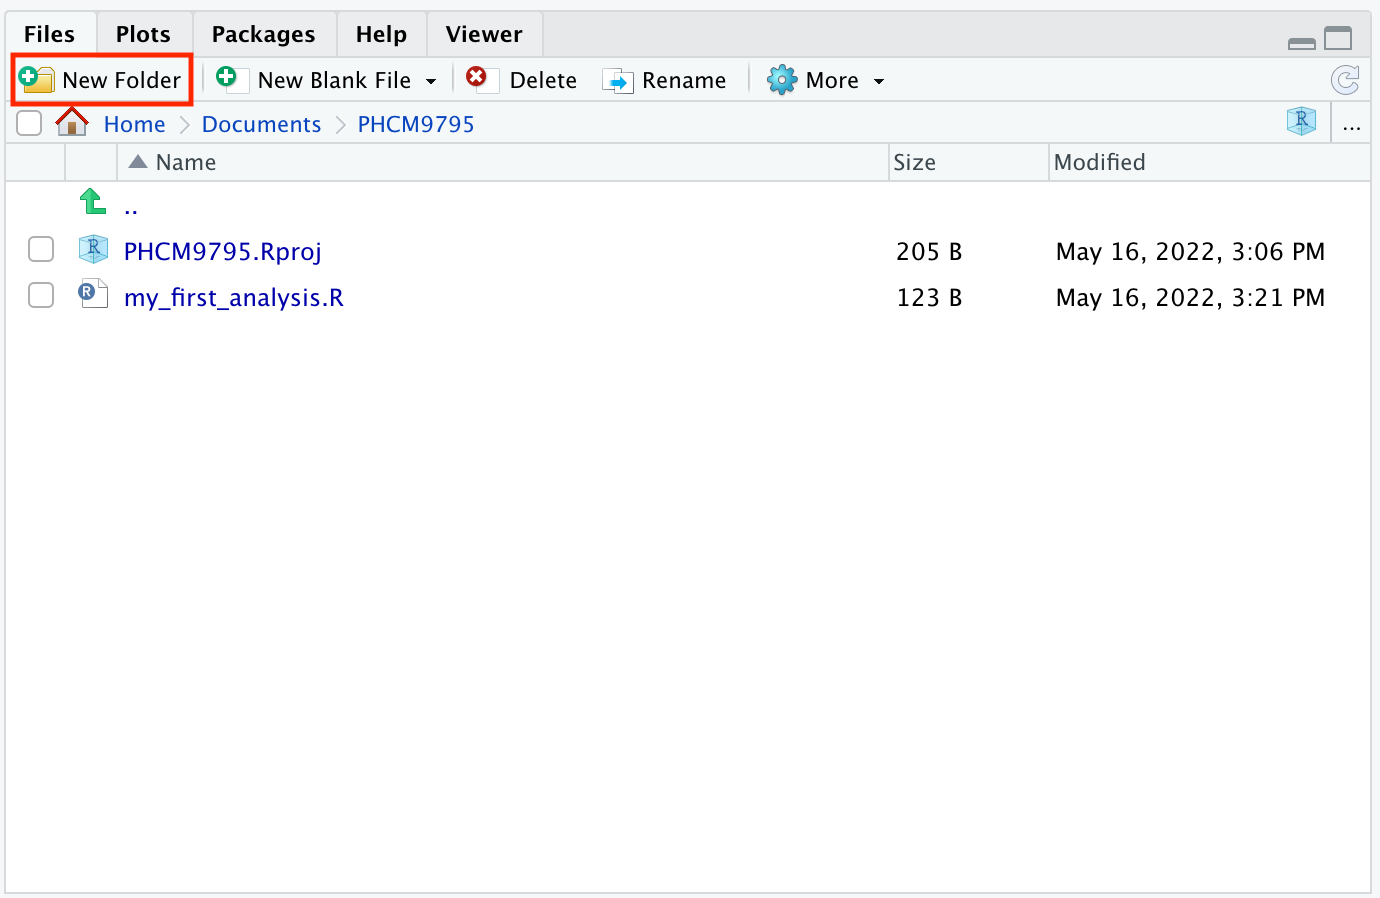
\includegraphics[width=0.75\linewidth]{img/NewFolder-1}

Call the new folder \textbf{data}.

Click on this folder to open it, and then create two new folders: \textbf{activities} and \textbf{examples}.

Download the ``Data sets: for learning activities'' from Moodle, and use Windows Explorer or MacOS Finder to save these data sets in \textbf{activities}. Save the ``Data sets: example data from course notes'' into the \textbf{examples} folder.

Your \textbf{activities} folder should look like:

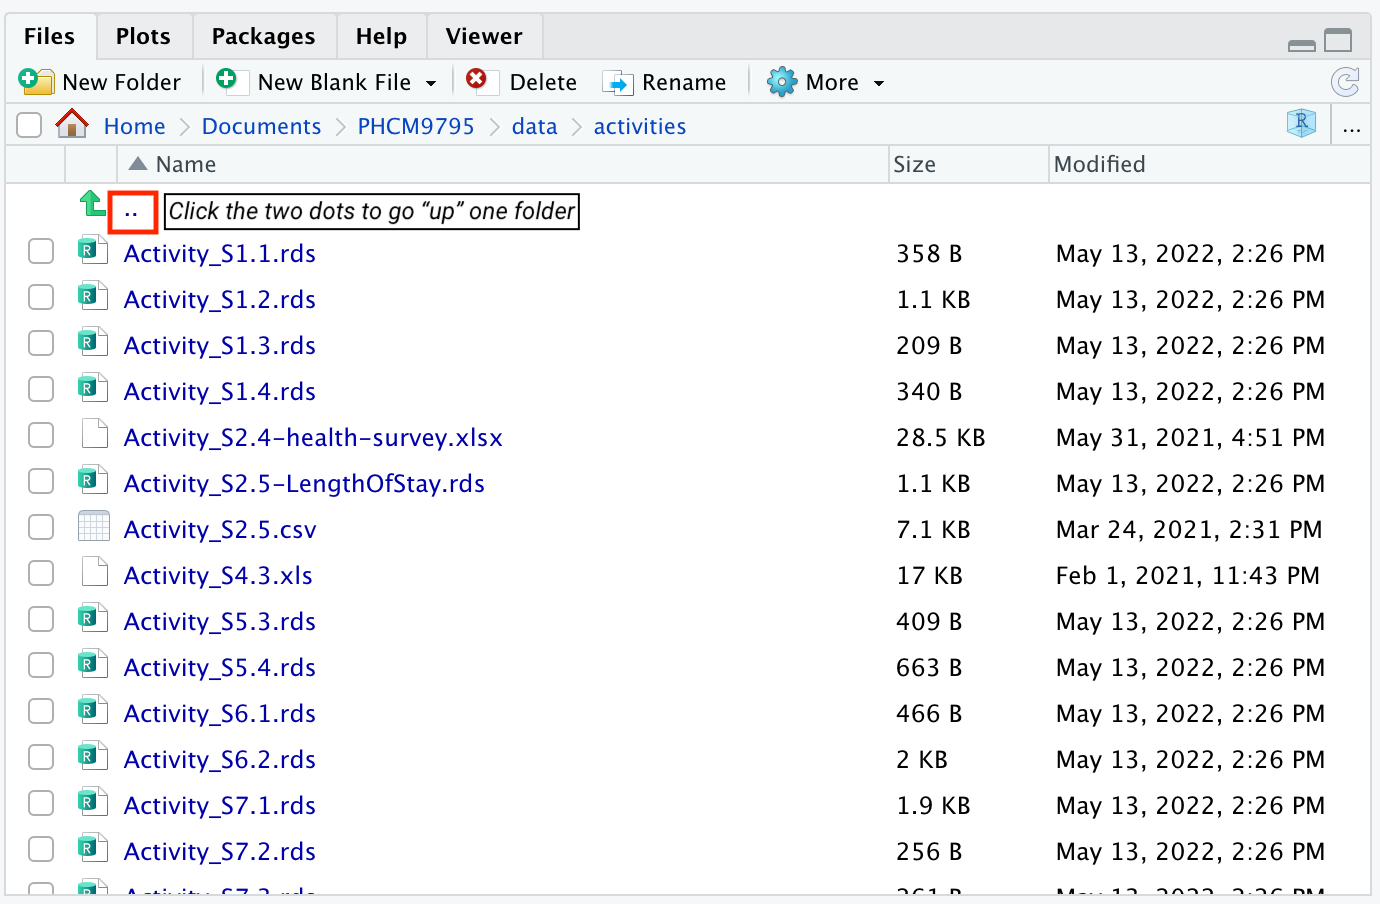
\includegraphics[width=0.75\linewidth]{img/data-folder}

Click the two dots next to the up-arrow at the top of the folder contents to move back up the folder structure. Note that you need to click the dots, and not the up-facing green arrow!

\hypertarget{reading-a-data-file}{%
\section{Reading a data file}\label{reading-a-data-file}}

Typing data directly into R is not common; we usually read data that have been previously saved. In this example, we will read an \texttt{.rds} file using the \texttt{readRDS()} function, which has only one input: the location of the file.

1 - Confirm that the \texttt{pbc.rds} file is in the \texttt{activities} sub-folder within the \texttt{data} folder (as per the previous steps).

2 - Install the packages: \texttt{jmv}, \texttt{skimr} and \texttt{summarytools} using \textbf{Tools \textgreater{} Install packages}, or by typing into the console:

\texttt{install.packages("jmv")}

\texttt{install.packages("skimr")}

\texttt{install.packages("summarytools")}

3 - Load the \texttt{skimr} package, and use the \texttt{readRDS()} function to read the file into R, assigning it to a data frame called \texttt{pbc}. Because we set up our project, we can locate our data easily by telling R to use the file: \texttt{"data/activities/pbc.rds"}, which translates as: the file \texttt{pbc.rds} which is located in the \texttt{activities} sub-folder within the \texttt{data} folder.

\begin{Shaded}
\begin{Highlighting}[]
\FunctionTok{library}\NormalTok{(skimr)}

\NormalTok{pbc }\OtherTok{\textless{}{-}} \FunctionTok{readRDS}\NormalTok{(}\StringTok{"data/activities/pbc.rds"}\NormalTok{)}
\end{Highlighting}
\end{Shaded}

4 - We can now use the \texttt{summary()} function to examine the pbc dataset:

\begin{Shaded}
\begin{Highlighting}[]
\FunctionTok{summary}\NormalTok{(pbc)}
\end{Highlighting}
\end{Shaded}

\begin{verbatim}
##        id             time          status            trt       
##  Min.   :  1.0   Min.   :  41   Min.   :0.0000   Min.   :1.000  
##  1st Qu.:105.2   1st Qu.:1093   1st Qu.:0.0000   1st Qu.:1.000  
##  Median :209.5   Median :1730   Median :0.0000   Median :1.000  
##  Mean   :209.5   Mean   :1918   Mean   :0.8301   Mean   :1.494  
##  3rd Qu.:313.8   3rd Qu.:2614   3rd Qu.:2.0000   3rd Qu.:2.000  
##  Max.   :418.0   Max.   :4795   Max.   :2.0000   Max.   :2.000  
##                                                  NA's   :106    
##       age             sex           ascites            hepato      
##  Min.   :26.28   Min.   :1.000   Min.   :0.00000   Min.   :0.0000  
##  1st Qu.:42.83   1st Qu.:2.000   1st Qu.:0.00000   1st Qu.:0.0000  
##  Median :51.00   Median :2.000   Median :0.00000   Median :1.0000  
##  Mean   :50.74   Mean   :1.895   Mean   :0.07692   Mean   :0.5128  
##  3rd Qu.:58.24   3rd Qu.:2.000   3rd Qu.:0.00000   3rd Qu.:1.0000  
##  Max.   :78.44   Max.   :2.000   Max.   :1.00000   Max.   :1.0000  
##                                  NA's   :106       NA's   :106     
##     spiders           edema             bili             chol       
##  Min.   :0.0000   Min.   :0.0000   Min.   : 0.300   Min.   : 120.0  
##  1st Qu.:0.0000   1st Qu.:0.0000   1st Qu.: 0.800   1st Qu.: 249.5  
##  Median :0.0000   Median :0.0000   Median : 1.400   Median : 309.5  
##  Mean   :0.2885   Mean   :0.1005   Mean   : 3.221   Mean   : 369.5  
##  3rd Qu.:1.0000   3rd Qu.:0.0000   3rd Qu.: 3.400   3rd Qu.: 400.0  
##  Max.   :1.0000   Max.   :1.0000   Max.   :28.000   Max.   :1775.0  
##  NA's   :106                                        NA's   :134     
##     albumin          copper          alkphos             ast        
##  Min.   :1.960   Min.   :  4.00   Min.   :  289.0   Min.   : 26.35  
##  1st Qu.:3.243   1st Qu.: 41.25   1st Qu.:  871.5   1st Qu.: 80.60  
##  Median :3.530   Median : 73.00   Median : 1259.0   Median :114.70  
##  Mean   :3.497   Mean   : 97.65   Mean   : 1982.7   Mean   :122.56  
##  3rd Qu.:3.770   3rd Qu.:123.00   3rd Qu.: 1980.0   3rd Qu.:151.90  
##  Max.   :4.640   Max.   :588.00   Max.   :13862.4   Max.   :457.25  
##                  NA's   :108      NA's   :106       NA's   :106     
##       trig           platelet        protime          stage      
##  Min.   : 33.00   Min.   : 62.0   Min.   : 9.00   Min.   :1.000  
##  1st Qu.: 84.25   1st Qu.:188.5   1st Qu.:10.00   1st Qu.:2.000  
##  Median :108.00   Median :251.0   Median :10.60   Median :3.000  
##  Mean   :124.70   Mean   :257.0   Mean   :10.73   Mean   :3.024  
##  3rd Qu.:151.00   3rd Qu.:318.0   3rd Qu.:11.10   3rd Qu.:4.000  
##  Max.   :598.00   Max.   :721.0   Max.   :18.00   Max.   :4.000  
##  NA's   :136      NA's   :11      NA's   :2       NA's   :6
\end{verbatim}

An alternative to the \texttt{summary()} function is the \texttt{skim()} function in the \texttt{skimr} package, which produces summary statistics as well as rudimentary histograms:

\begin{Shaded}
\begin{Highlighting}[]
\FunctionTok{skim}\NormalTok{(pbc)}
\end{Highlighting}
\end{Shaded}

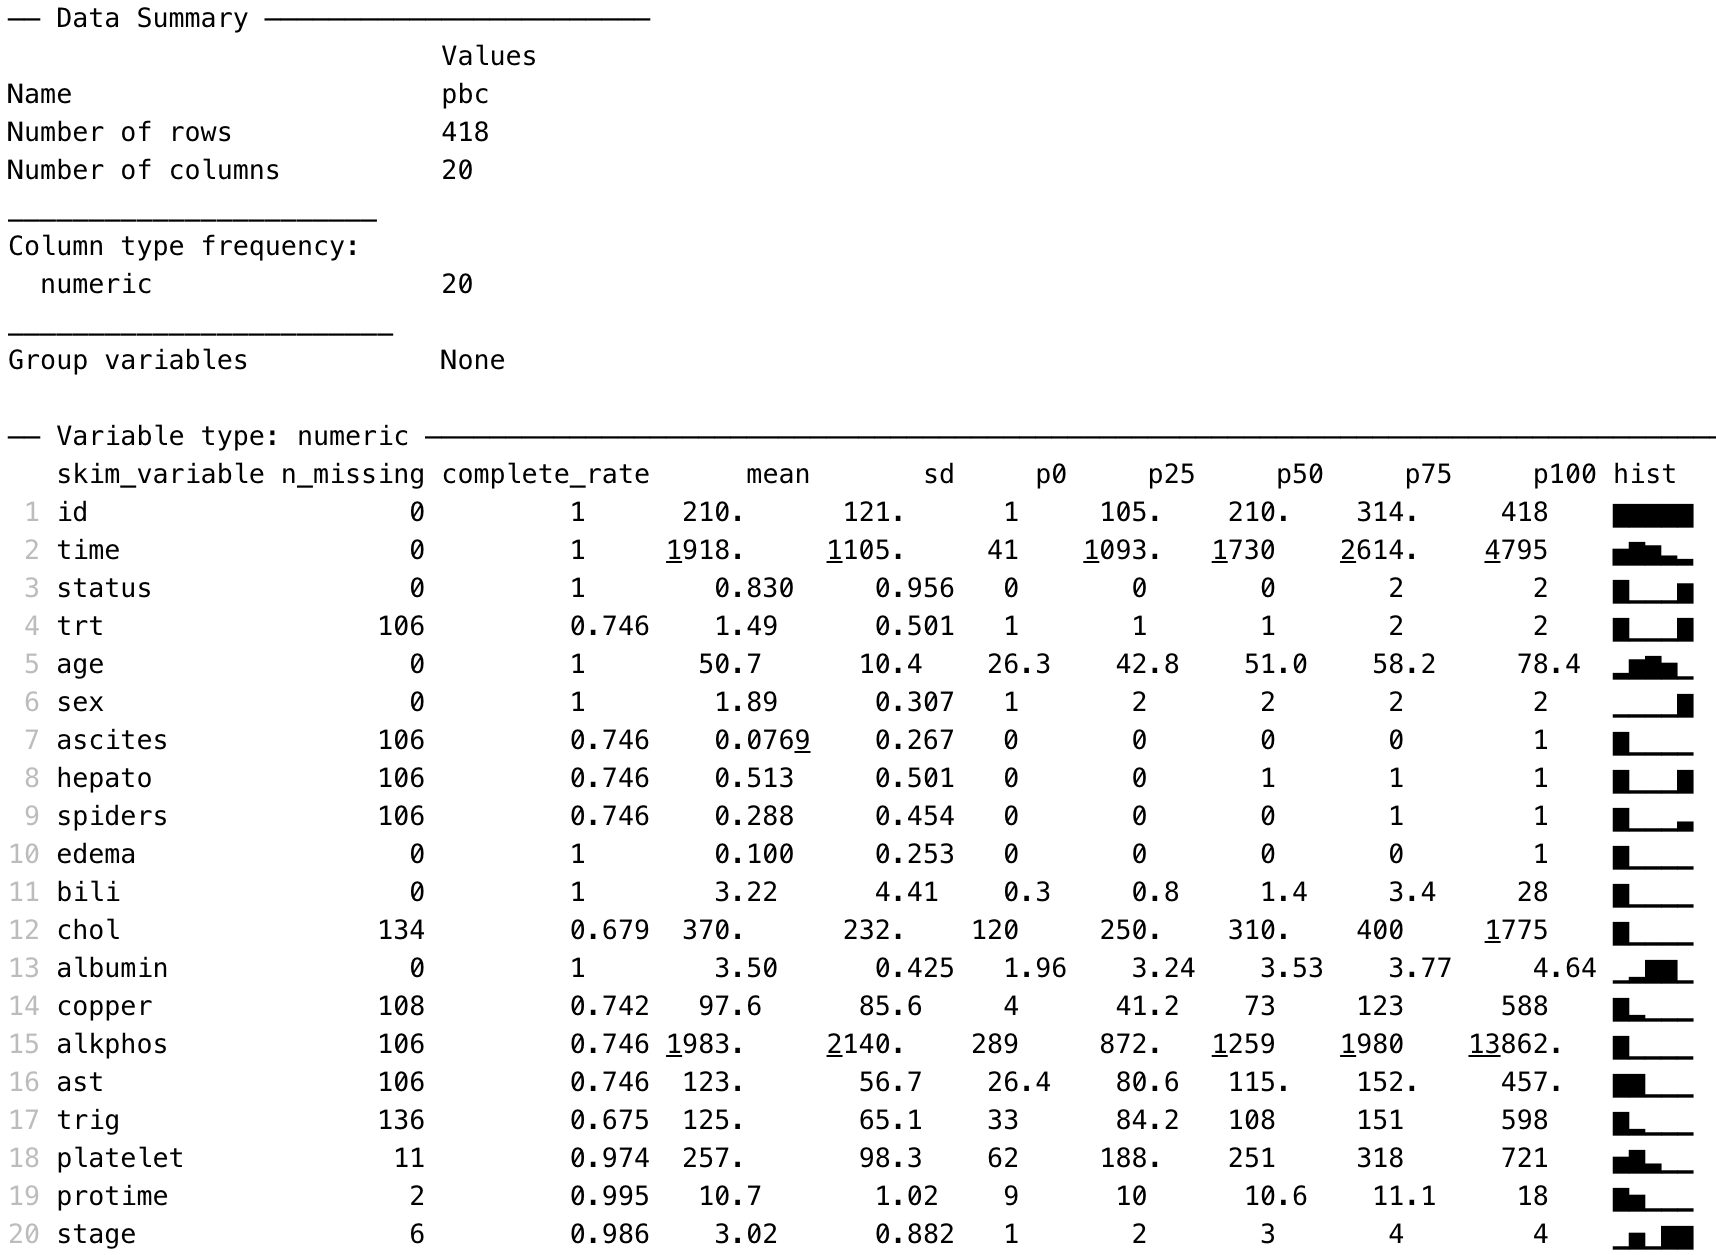
\includegraphics[width=0.9\linewidth]{img/skim-pbc}

The \texttt{summary()} and \texttt{skim()} functions are useful to give a quick overview of a dataset: how many variables are included, how variables are coded, which variables contain missing data and a crude histogram showing the distribution of numeric variables.

\hypertarget{summarising-continuous-variables}{%
\section{Summarising continuous variables}\label{summarising-continuous-variables}}

One of the most flexible functions for summarising continuous variables is the \texttt{descriptives()} function from the \texttt{jmv} package. The function is specified as \texttt{descriptives(data=,\ vars=)} where:

\begin{itemize}
\tightlist
\item
  \texttt{data} specifies the dataframe to be analysed
\item
  \texttt{vars} specifies the variable(s) of interest, with multiple variables combined using the \texttt{c()} function
\end{itemize}

We can summarise the three continuous variables in the pbc data: age, AST and serum bilirubin, as shown below.

\begin{Shaded}
\begin{Highlighting}[]
\FunctionTok{library}\NormalTok{(jmv)}

\FunctionTok{descriptives}\NormalTok{(}\AttributeTok{data=}\NormalTok{pbc, }\AttributeTok{vars=}\FunctionTok{c}\NormalTok{(age, ast, bili))}
\end{Highlighting}
\end{Shaded}

\begin{verbatim}
## 
##  DESCRIPTIVES
## 
##  Descriptives                                                
##  ─────────────────────────────────────────────────────────── 
##                          age         ast         bili        
##  ─────────────────────────────────────────────────────────── 
##    N                          418         312          418   
##    Missing                      0         106            0   
##    Mean                  50.74155    122.5563     3.220813   
##    Median                51.00068    114.7000     1.400000   
##    Standard deviation    10.44721    56.69952     4.407506   
##    Minimum               26.27789    26.35000    0.3000000   
##    Maximum               78.43943    457.2500     28.00000   
##  ───────────────────────────────────────────────────────────
\end{verbatim}

By default, the \texttt{descriptives} function presents the mean, median, standard deviation, minimum and maximum. We can request additional statistics, such as the quartiles (which are called the percentiles, or pc, in the descriptives function):

\begin{Shaded}
\begin{Highlighting}[]
\FunctionTok{descriptives}\NormalTok{(}\AttributeTok{data=}\NormalTok{pbc, }\AttributeTok{vars=}\FunctionTok{c}\NormalTok{(age, ast, bili), }\AttributeTok{pc=}\ConstantTok{TRUE}\NormalTok{)}
\end{Highlighting}
\end{Shaded}

\begin{verbatim}
## 
##  DESCRIPTIVES
## 
##  Descriptives                                                
##  ─────────────────────────────────────────────────────────── 
##                          age         ast         bili        
##  ─────────────────────────────────────────────────────────── 
##    N                          418         312          418   
##    Missing                      0         106            0   
##    Mean                  50.74155    122.5563     3.220813   
##    Median                51.00068    114.7000     1.400000   
##    Standard deviation    10.44721    56.69952     4.407506   
##    Minimum               26.27789    26.35000    0.3000000   
##    Maximum               78.43943    457.2500     28.00000   
##    25th percentile       42.83231    80.60000    0.8000000   
##    50th percentile       51.00068    114.7000     1.400000   
##    75th percentile       58.24093    151.9000     3.400000   
##  ───────────────────────────────────────────────────────────
\end{verbatim}

\hypertarget{producing-a-histogram}{%
\section{Producing a histogram}\label{producing-a-histogram}}

We can use the \texttt{hist()} function to produce a histogram, specifying the dataframe to use and the variable to be plotted as \texttt{dataframe\$variable}:

\begin{Shaded}
\begin{Highlighting}[]
\FunctionTok{hist}\NormalTok{(pbc}\SpecialCharTok{$}\NormalTok{age)}
\end{Highlighting}
\end{Shaded}

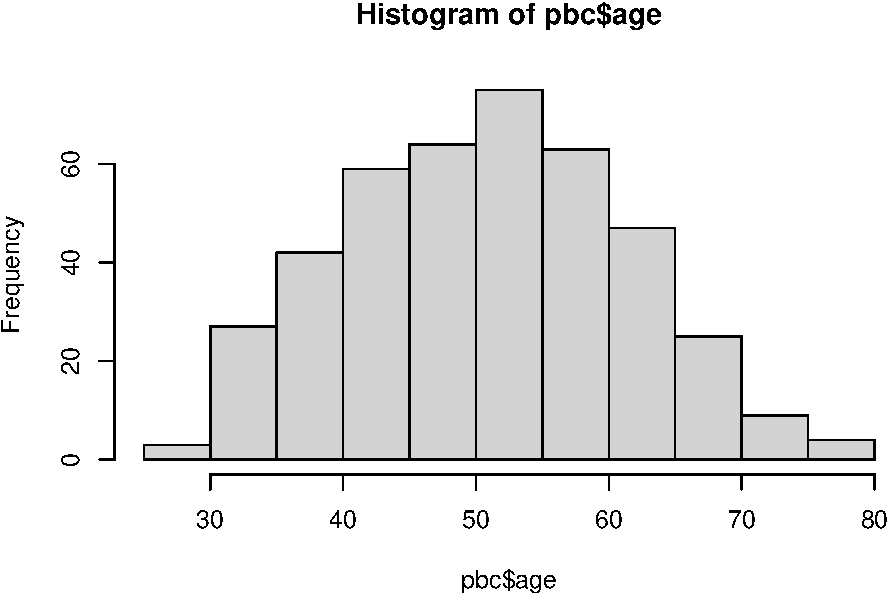
\includegraphics{phcm9795-R-notes_files/figure-latex/unnamed-chunk-32-1.pdf}

The histogram function does a remarkably good job of choosing cutpoints and binwidths, and these rarely need to be changed. However, the labelling of the histogram should be improved by using \texttt{xlab="\ "} and \texttt{main="\ "} to assign labels for the x-axis and overall title respectively:

\begin{Shaded}
\begin{Highlighting}[]
\FunctionTok{hist}\NormalTok{(pbc}\SpecialCharTok{$}\NormalTok{age, }\AttributeTok{xlab=}\StringTok{"Age (years)"}\NormalTok{, }
     \AttributeTok{main=}\StringTok{"Histogram of participant age from pbc study data"}\NormalTok{)}
\end{Highlighting}
\end{Shaded}

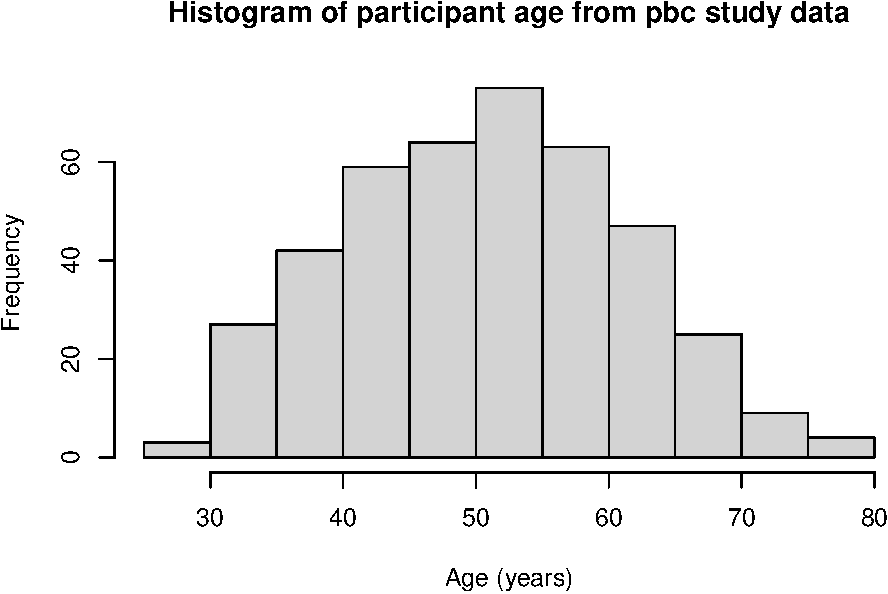
\includegraphics{phcm9795-R-notes_files/figure-latex/unnamed-chunk-33-1.pdf}

By default, the \texttt{hist()} function plots a \textbf{frequency histogram}, with counts on the y-axis. We can tweak the histogram using the following code to plot a histogram of the \textbf{relative frequencies}:

\begin{Shaded}
\begin{Highlighting}[]
\NormalTok{h }\OtherTok{\textless{}{-}} \FunctionTok{hist}\NormalTok{(pbc}\SpecialCharTok{$}\NormalTok{age, }\AttributeTok{plot=}\ConstantTok{FALSE}\NormalTok{)}
\NormalTok{h}\SpecialCharTok{$}\NormalTok{density }\OtherTok{\textless{}{-}}\NormalTok{ h}\SpecialCharTok{$}\NormalTok{counts}\SpecialCharTok{/}\FunctionTok{sum}\NormalTok{(h}\SpecialCharTok{$}\NormalTok{counts)}\SpecialCharTok{*}\DecValTok{100}
\FunctionTok{plot}\NormalTok{(h, }\AttributeTok{freq=}\ConstantTok{FALSE}\NormalTok{, }
     \AttributeTok{xlab=}\StringTok{"Age (years)"}\NormalTok{, }
     \AttributeTok{ylab=}\StringTok{"Relative frequency (\%)"}\NormalTok{,}
     \AttributeTok{main=}\StringTok{"Histogram of participant age from pbc study data"}\NormalTok{)}
\end{Highlighting}
\end{Shaded}

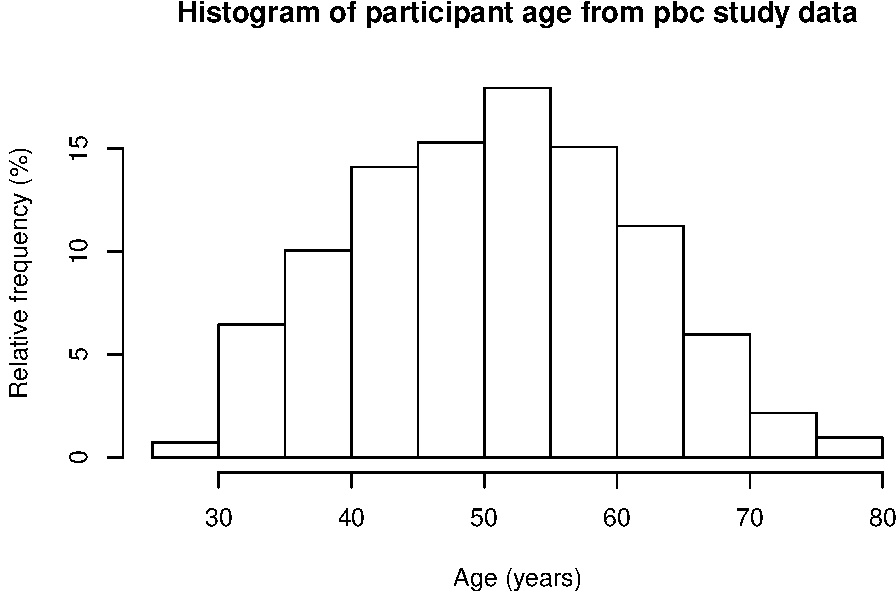
\includegraphics{phcm9795-R-notes_files/figure-latex/unnamed-chunk-34-1.pdf}

\hypertarget{producing-a-boxplot}{%
\section{Producing a boxplot}\label{producing-a-boxplot}}

The \texttt{boxplot} function is used to produce boxplots, again specifying the dataframe to use and the variable to be plotted as \texttt{dataframe\$variable}. Labels can be applied in the same way as the histogram:

\begin{Shaded}
\begin{Highlighting}[]
\FunctionTok{boxplot}\NormalTok{(pbc}\SpecialCharTok{$}\NormalTok{age, }\AttributeTok{xlab=}\StringTok{"Age (years)"}\NormalTok{, }\AttributeTok{main=}\StringTok{"Boxplot of participant age from pbc study data"}\NormalTok{)}
\end{Highlighting}
\end{Shaded}

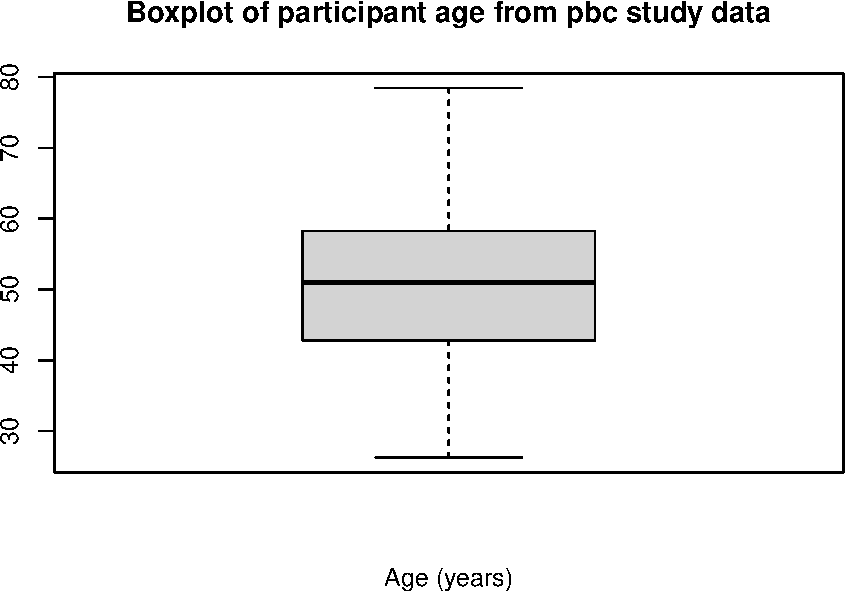
\includegraphics{phcm9795-R-notes_files/figure-latex/unnamed-chunk-35-1.pdf}

\hypertarget{producing-a-one-way-frequency-table}{%
\section{Producing a one-way frequency table}\label{producing-a-one-way-frequency-table}}

We have three categorical variables to summarise in Table 1: sex, stage and vital status. These variables are best summarised using one-way frequency tables.

\begin{Shaded}
\begin{Highlighting}[]
\FunctionTok{library}\NormalTok{(summarytools)}

\FunctionTok{freq}\NormalTok{(pbc}\SpecialCharTok{$}\NormalTok{sex)}
\end{Highlighting}
\end{Shaded}

\begin{verbatim}
## Frequencies  
## pbc$sex  
## Type: Numeric  
## 
##               Freq   % Valid   % Valid Cum.   % Total   % Total Cum.
## ----------- ------ --------- -------------- --------- --------------
##           1     44     10.53          10.53     10.53          10.53
##           2    374     89.47         100.00     89.47         100.00
##        <NA>      0                               0.00         100.00
##       Total    418    100.00         100.00    100.00         100.00
\end{verbatim}

\hypertarget{defining-categorical-variables-as-factors}{%
\subsection{Defining categorical variables as factors}\label{defining-categorical-variables-as-factors}}

You will notice that the table above, in its current form, is uninterpretable as the 1 and 2 categories are not labelled. In this course, all variables including categorical variables tend to be numerically coded. To define a categorical variable as such in R, we define it as a \textbf{factor} using the factor function:

\texttt{factor(variable=,\ levels=,\ labels=)}

We specify:

\begin{itemize}
\tightlist
\item
  levels: the values the categorical variable can take
\item
  labels: the labels corresponding to each of the levels (entered in the same order as the levels)
\end{itemize}

To define our variable sex as a factor, we use:

\begin{Shaded}
\begin{Highlighting}[]
\NormalTok{pbc}\SpecialCharTok{$}\NormalTok{sex }\OtherTok{\textless{}{-}} \FunctionTok{factor}\NormalTok{(pbc}\SpecialCharTok{$}\NormalTok{sex, }\AttributeTok{levels=}\FunctionTok{c}\NormalTok{(}\DecValTok{1}\NormalTok{, }\DecValTok{2}\NormalTok{), }\AttributeTok{labels=}\FunctionTok{c}\NormalTok{(}\StringTok{"Male"}\NormalTok{, }\StringTok{"Female"}\NormalTok{))}
\end{Highlighting}
\end{Shaded}

We can confirm the coding by re-running a frequency table:

\begin{Shaded}
\begin{Highlighting}[]
\FunctionTok{freq}\NormalTok{(pbc}\SpecialCharTok{$}\NormalTok{sex)}
\end{Highlighting}
\end{Shaded}

\begin{verbatim}
## Frequencies  
## pbc$sex  
## Type: Factor  
## 
##                Freq   % Valid   % Valid Cum.   % Total   % Total Cum.
## ------------ ------ --------- -------------- --------- --------------
##         Male     44     10.53          10.53     10.53          10.53
##       Female    374     89.47         100.00     89.47         100.00
##         <NA>      0                               0.00         100.00
##        Total    418    100.00         100.00    100.00         100.00
\end{verbatim}

\begin{quote}
Task: define \texttt{stage} and \texttt{status} (Vital Status) as factors, and produce one-way frequency tables. Refer to the file \texttt{pbc\_info.txt} to view the labels for each variable. For example, for Stage:
\end{quote}

\begin{Shaded}
\begin{Highlighting}[]
\NormalTok{pbc}\SpecialCharTok{$}\NormalTok{stage }\OtherTok{\textless{}{-}} \FunctionTok{factor}\NormalTok{(pbc}\SpecialCharTok{$}\NormalTok{stage, }\AttributeTok{levels=}\FunctionTok{c}\NormalTok{(}\DecValTok{1}\NormalTok{, }\DecValTok{2}\NormalTok{, }\DecValTok{3}\NormalTok{, }\DecValTok{4}\NormalTok{), }\AttributeTok{labels=}\FunctionTok{c}\NormalTok{(}\StringTok{"Stage 1"}\NormalTok{, }\StringTok{"Stage 2"}\NormalTok{, }\StringTok{"Stage 3"}\NormalTok{, }\StringTok{"Stage 4"}\NormalTok{))}
\FunctionTok{freq}\NormalTok{(pbc}\SpecialCharTok{$}\NormalTok{stage)}
\end{Highlighting}
\end{Shaded}

\begin{verbatim}
## Frequencies  
## pbc$stage  
## Type: Factor  
## 
##                 Freq   % Valid   % Valid Cum.   % Total   % Total Cum.
## ------------- ------ --------- -------------- --------- --------------
##       Stage 1     21      5.10           5.10      5.02           5.02
##       Stage 2     92     22.33          27.43     22.01          27.03
##       Stage 3    155     37.62          65.05     37.08          64.11
##       Stage 4    144     34.95         100.00     34.45          98.56
##          <NA>      6                               1.44         100.00
##         Total    418    100.00         100.00    100.00         100.00
\end{verbatim}

\hypertarget{producing-a-two-way-frequency-table}{%
\section{Producing a two-way frequency table}\label{producing-a-two-way-frequency-table}}

To produce tables summarising two categorical variables, we can use the \texttt{contTables()} function within the \texttt{jmv} package. The minimal inputs to include are \texttt{data}: the name of the data frame to be analysed, \texttt{rows}: the variable representing the rows of the table, and \texttt{cols}: the name of the columns of the table.

For example, to produce a two-way table showing stage of disease by sex using the pbc data frame, we use:

\begin{Shaded}
\begin{Highlighting}[]
\FunctionTok{contTables}\NormalTok{(}\AttributeTok{data=}\NormalTok{pbc, }\AttributeTok{rows=}\NormalTok{sex, }\AttributeTok{cols=}\NormalTok{stage)}
\end{Highlighting}
\end{Shaded}

\begin{verbatim}
## 
##  CONTINGENCY TABLES
## 
##  Contingency Tables                                              
##  ─────────────────────────────────────────────────────────────── 
##    sex       Stage 1    Stage 2    Stage 3    Stage 4    Total   
##  ─────────────────────────────────────────────────────────────── 
##    Male            3          8         16         17       44   
##    Female         18         84        139        127      368   
##    Total          21         92        155        144      412   
##  ─────────────────────────────────────────────────────────────── 
## 
## 
##  χ² Tests                               
##  ────────────────────────────────────── 
##          Value        df    p           
##  ────────────────────────────────────── 
##    χ²    0.8779873     3    0.8307365   
##    N           412                      
##  ──────────────────────────────────────
\end{verbatim}

{[}The bottom part of the output, χ² Tests, can be ignored for now{]}

You may notice in the above that the number of observations is now 412. This is because there are missing observations for either sex or stage: which is it, and how would you determine this?

From the cross-tabulation, you can see the individual frequencies of participants in each of the categories in each cell. For example, there are 3 male participants who have Stage 1 disease. You can also read the totals for each row and column. For example, there are 44 males, and 144 participants have Stage 4 disease.

You can also add percentages into your table using \texttt{pcCol=TRUE} to include column percents, and \texttt{pcRow=TRUE} for row percents. For example, to calculate the relative frequencies (i.e.~percentages) of sex within each stage, we would request \textbf{column percents} with the option: \texttt{pcCol=TRUE}.

\begin{Shaded}
\begin{Highlighting}[]
\FunctionTok{contTables}\NormalTok{(}\AttributeTok{data=}\NormalTok{pbc, }\AttributeTok{rows=}\NormalTok{sex, }\AttributeTok{cols=}\NormalTok{stage, }\AttributeTok{pcCol=}\ConstantTok{TRUE}\NormalTok{)}
\end{Highlighting}
\end{Shaded}

\begin{verbatim}
## 
##  CONTINGENCY TABLES
## 
##  Contingency Tables                                                                             
##  ────────────────────────────────────────────────────────────────────────────────────────────── 
##    sex                          Stage 1      Stage 2      Stage 3      Stage 4      Total       
##  ────────────────────────────────────────────────────────────────────────────────────────────── 
##    Male      Observed                   3            8           16           17           44   
##              % within column     14.28571      8.69565     10.32258     11.80556     10.67961   
##                                                                                                 
##    Female    Observed                  18           84          139          127          368   
##              % within column     85.71429     91.30435     89.67742     88.19444     89.32039   
##                                                                                                 
##    Total     Observed                  21           92          155          144          412   
##              % within column    100.00000    100.00000    100.00000    100.00000    100.00000   
##  ────────────────────────────────────────────────────────────────────────────────────────────── 
## 
## 
##  χ² Tests                               
##  ────────────────────────────────────── 
##          Value        df    p           
##  ────────────────────────────────────── 
##    χ²    0.8779873     3    0.8307365   
##    N           412                      
##  ──────────────────────────────────────
\end{verbatim}

We can see that the 3 male participants with Stage 1 disease represent 14\% of those with Stage 1 disease.

\hypertarget{saving-data-in-r}{%
\section{Saving data in R}\label{saving-data-in-r}}

There are many ways to save data from R, depending on the type of file you want to save. The recommendation for this course is to save your data using the \texttt{.rds} format, using the \texttt{saveRDS()} function, which takes two inputs: \texttt{saveRDS(object,\ file)}. Here, \texttt{object} is the R object to be saved (usually a data frame), and \texttt{file} is the location for the file to be saved (file name and path, including the \texttt{.rds} suffix).

It is not necessary to save our PBC data, as we have made only minor changes to the data that can be replicated by rerunning our script. If you had made major changes and wanted to save your data, you could use:

\texttt{saveRDS(pbc,\ file="pbc\_revised.rds")}

\hypertarget{copying-output-from-r}{%
\section{Copying output from R}\label{copying-output-from-r}}

It is important to note that saving your data or your script in R will not save your output. The easiest way to retain the output of your analyses is to copy the output from the Console into a word processor package (e.g.~Microsoft Word) before closing R.

Unfortunately, by default, R is not ideal for creating publication quality tables. There are many packages that will help in this process, such as R Markdown, bookdown\footnote{these R notes and the PHCM9795 course notes have been written using \href{https://bookdown.org/yihui/bookdown/}{bookdown}}, huxtable, gt and gtsummary, but their use is beyond the scope of this course. \href{https://rmd4sci.njtierney.com/}{R Markdown for Scientists} provides an excellent introduction to R Markdown.

\begin{quote}
Task: Complete Table 1 using the output generated in this exercise. You should decide on whether to present continuous variables by their means or medians, and present the most appropriate measure of spread. Include footnotes to indicate if any variables contain missing observations.
\end{quote}

\hypertarget{part-3-creating-other-types-of-graphs}{%
\section*{Part 3: Creating other types of graphs}\label{part-3-creating-other-types-of-graphs}}
\addcontentsline{toc}{section}{Part 3: Creating other types of graphs}

The \texttt{plot()} function, also known as \emph{base graphics}, is the default method of plotting data in R that can produce publication-quality graphics with minimal coding. There are alternative packages for plotting, with \texttt{ggplot2} being one of the most well known. We will present instructions for base graphics in this course, but excellent documentation for \texttt{ggplot2} can be found at the \href{https://ggplot2-book.org/}{ggplot2: Elegant Graphics for Data Analysis} website, written by the package authors.

\hypertarget{bar-graphs}{%
\section{Bar graphs}\label{bar-graphs}}

The simplest way to use the \texttt{plot()} function is by specifying an object to be plotted. As with the \texttt{hist()} function, to plot a single variable from a data frame, we must define it using: \texttt{dataframe\$variable}.

Here we will create the bar chart shown in Figure 1.3 of the statistics notes using the \texttt{pbc.rds} dataset. The x-axis of this graph will be the stage of disease, and the y-axis will show the number of participants in each category.

\begin{Shaded}
\begin{Highlighting}[]
\FunctionTok{plot}\NormalTok{(pbc}\SpecialCharTok{$}\NormalTok{stage, }
     \AttributeTok{main=}\StringTok{"Bar graph of stage of disease from PBC study"}\NormalTok{, }
     \AttributeTok{ylab=}\StringTok{"Number of participants"}\NormalTok{)}
\end{Highlighting}
\end{Shaded}

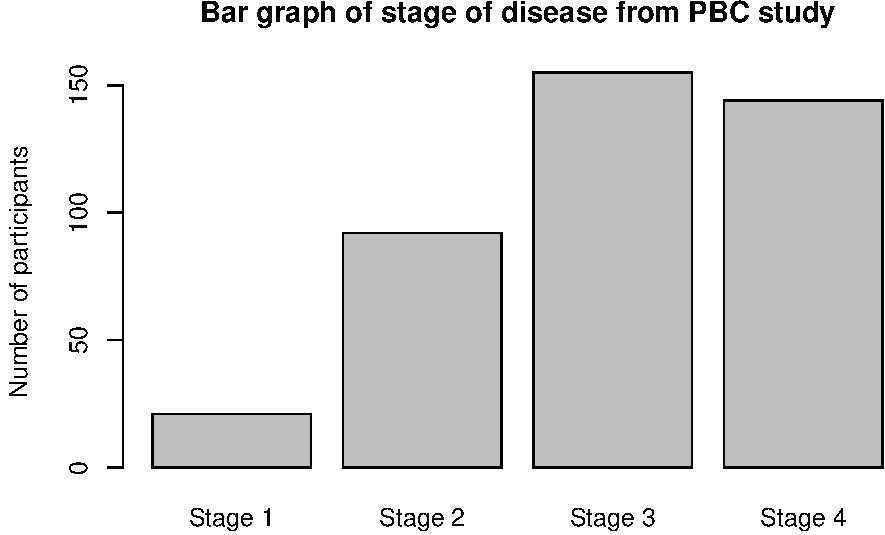
\includegraphics{phcm9795-R-notes_files/figure-latex/unnamed-chunk-42-1.pdf}

Note that stage is a categorical variable, that has been defined as a factor (in Section \ref{defining-categorical-variables-as-factors}). You \textbf{must define categorical data as factors} to plot them in a bar graph.

\hypertarget{clustered-bar-graph}{%
\subsection{Clustered bar graph}\label{clustered-bar-graph}}

To create a clustered bar chart as shown in Figure 1.4 of the statistics notes, we need to do a bit of manipulation. We first need to tabulate the data using the \texttt{table()} function. We want to plot stage of disease broken down by sex, so we specify \texttt{sex} as the first variable, and \texttt{stage} as the second variable for the \texttt{table()} command.

\begin{Shaded}
\begin{Highlighting}[]
\NormalTok{counts }\OtherTok{\textless{}{-}} \FunctionTok{table}\NormalTok{(pbc}\SpecialCharTok{$}\NormalTok{sex, pbc}\SpecialCharTok{$}\NormalTok{stage)}
\NormalTok{counts}
\end{Highlighting}
\end{Shaded}

\begin{verbatim}
##         
##          Stage 1 Stage 2 Stage 3 Stage 4
##   Male         3       8      16      17
##   Female      18      84     139     127
\end{verbatim}

After tabulating the data, we use the \texttt{barplot()} function to plot the summarised data. We specify the main title using \texttt{main="\ "}, specify that the stages be plotted separately by sex (\texttt{beside=TRUE}), specify the legend be defined by sex, and position the legend in the top-left of the graph:

\begin{Shaded}
\begin{Highlighting}[]
\FunctionTok{barplot}\NormalTok{(counts, }\AttributeTok{main=}\StringTok{"Bar graph of stage of disease by sex from PBC study"}\NormalTok{,}
        \AttributeTok{beside=}\ConstantTok{TRUE}\NormalTok{, }\AttributeTok{legend =} \FunctionTok{rownames}\NormalTok{(counts), }\AttributeTok{args.legend =} \FunctionTok{list}\NormalTok{(}\AttributeTok{x =} \StringTok{"topleft"}\NormalTok{))}
\end{Highlighting}
\end{Shaded}

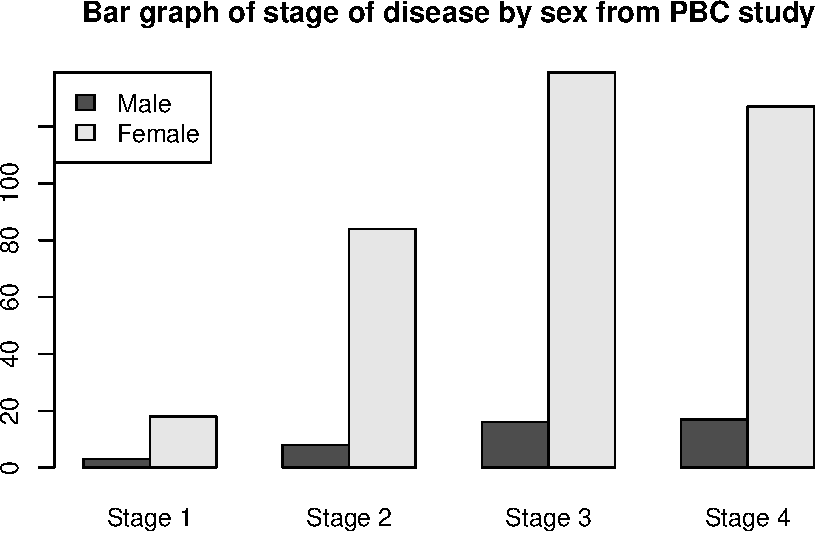
\includegraphics{phcm9795-R-notes_files/figure-latex/unnamed-chunk-44-1.pdf}

\hypertarget{stacked-bar-graph}{%
\subsection{Stacked bar graph}\label{stacked-bar-graph}}

A stacked bar graph can be constructed as for the clustered bar graph, but we specify \texttt{beside=FALSE}:

\begin{Shaded}
\begin{Highlighting}[]
\FunctionTok{barplot}\NormalTok{(counts, }\AttributeTok{main=}\StringTok{"Bar graph of stage of disease by sex from PBC study"}\NormalTok{,}
        \AttributeTok{beside=}\ConstantTok{FALSE}\NormalTok{, }\AttributeTok{legend =} \FunctionTok{rownames}\NormalTok{(counts), }\AttributeTok{args.legend =} \FunctionTok{list}\NormalTok{(}\AttributeTok{x =} \StringTok{"topleft"}\NormalTok{))}
\end{Highlighting}
\end{Shaded}

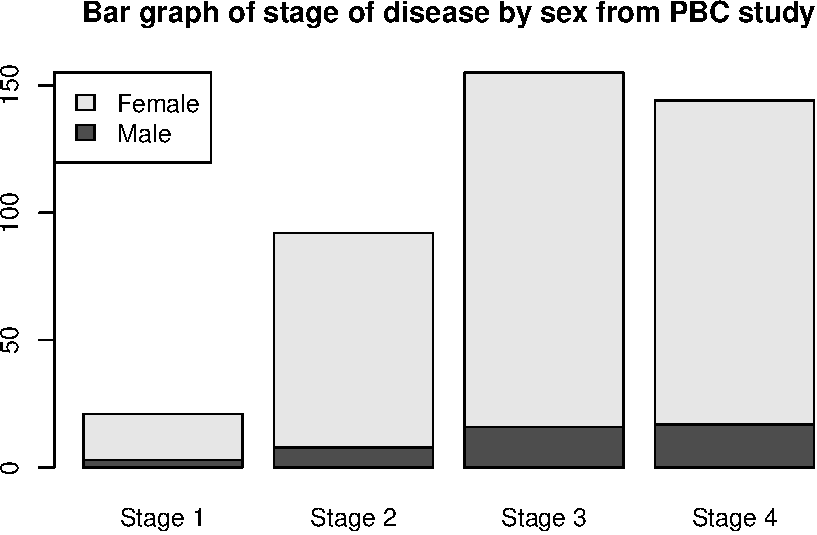
\includegraphics{phcm9795-R-notes_files/figure-latex/unnamed-chunk-45-1.pdf}

\hypertarget{stacked-bar-graph-of-relative-frequencies}{%
\subsection{Stacked bar graph of relative frequencies}\label{stacked-bar-graph-of-relative-frequencies}}

To plot relative frequencies, we need to transform our table of frequencies (\texttt{counts}) into proportions, by using the \texttt{prop.table()} function. The prop.table() function takes two arguments: a table of counts, and \texttt{margin}, which defines whether we want proportions calculated by row (\texttt{margin=1}) or column (\texttt{margin=2}).

We want to calculate the relative frequency of sex within each stage category. From our \texttt{counts} table above, this equates to calculating \emph{column} proportions, so we specify \texttt{margin=2}. We also multiply the resulting table by 100 to obtain percentages (rather than proportions):

\begin{Shaded}
\begin{Highlighting}[]
\NormalTok{percent }\OtherTok{\textless{}{-}} \FunctionTok{prop.table}\NormalTok{(counts, }\AttributeTok{margin=}\DecValTok{2}\NormalTok{)}\SpecialCharTok{*}\DecValTok{100}
\NormalTok{percent}
\end{Highlighting}
\end{Shaded}

\begin{verbatim}
##         
##            Stage 1   Stage 2   Stage 3   Stage 4
##   Male   14.285714  8.695652 10.322581 11.805556
##   Female 85.714286 91.304348 89.677419 88.194444
\end{verbatim}

After calculating the percentages, we use \texttt{barplot()} again, similar to the stacked bar graph:

\begin{Shaded}
\begin{Highlighting}[]
\FunctionTok{barplot}\NormalTok{(percent, }
        \AttributeTok{main=}\StringTok{"Relative frequency of sex within stage of disease from PBC study"}\NormalTok{,}
        \AttributeTok{legend =} \FunctionTok{rownames}\NormalTok{(counts), }\AttributeTok{beside=}\ConstantTok{FALSE}\NormalTok{, }\AttributeTok{args.legend =} \FunctionTok{list}\NormalTok{(}\AttributeTok{x =} \StringTok{"topright"}\NormalTok{))}
\end{Highlighting}
\end{Shaded}

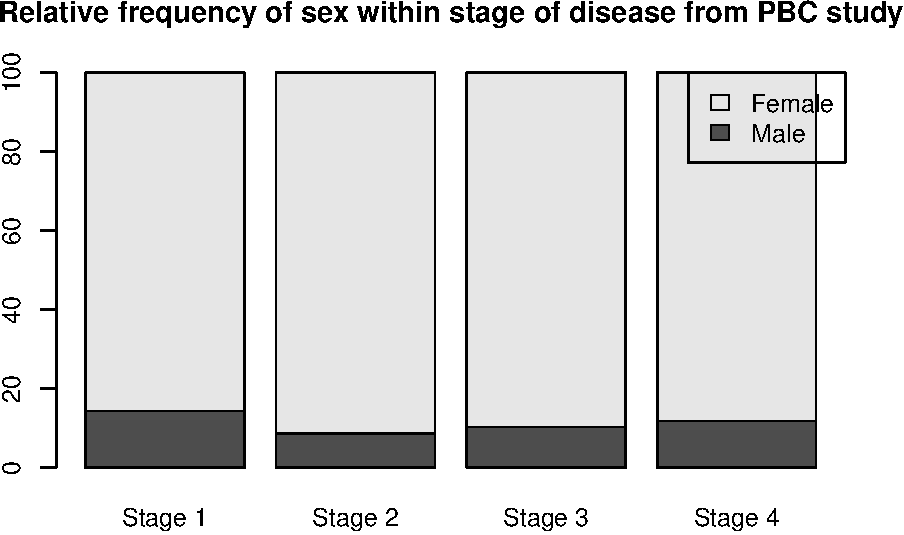
\includegraphics{phcm9795-R-notes_files/figure-latex/unnamed-chunk-47-1.pdf}

\hypertarget{creating-line-graphs}{%
\section{Creating line graphs}\label{creating-line-graphs}}

To demonstrate the graphing of aggregate data , we use the data on new cases and deaths from prostate cancer in males in NSW. This data has been entered as \texttt{Example\_1.2.rds}.

\begin{Shaded}
\begin{Highlighting}[]
\NormalTok{cancer }\OtherTok{\textless{}{-}} \FunctionTok{readRDS}\NormalTok{(}\StringTok{"data/examples/Example\_1.2.rds"}\NormalTok{)}
\FunctionTok{summary}\NormalTok{(cancer)}
\end{Highlighting}
\end{Shaded}

\begin{verbatim}
##       year          ncases        ndeaths           rcases         rdeaths     
##  Min.   :1987   Min.   :1567   Min.   : 645.0   Min.   : 81.8   Min.   :31.10  
##  1st Qu.:1992   1st Qu.:2804   1st Qu.: 788.2   1st Qu.:121.9   1st Qu.:34.67  
##  Median :1996   Median :3790   Median : 868.0   Median :131.3   Median :36.55  
##  Mean   :1996   Mean   :3719   Mean   : 855.0   Mean   :135.4   Mean   :37.09  
##  3rd Qu.:2001   3rd Qu.:4403   3rd Qu.: 921.0   3rd Qu.:164.2   3rd Qu.:40.38  
##  Max.   :2006   Max.   :6158   Max.   :1044.0   Max.   :186.9   Max.   :43.80
\end{verbatim}

We begin by plotting cancer cases (as the \emph{y} variable) against year (the \emph{x} variable).

\begin{Shaded}
\begin{Highlighting}[]
\FunctionTok{plot}\NormalTok{(}\AttributeTok{x=}\NormalTok{cancer}\SpecialCharTok{$}\NormalTok{year, }\AttributeTok{y=}\NormalTok{cancer}\SpecialCharTok{$}\NormalTok{rcases)}
\end{Highlighting}
\end{Shaded}

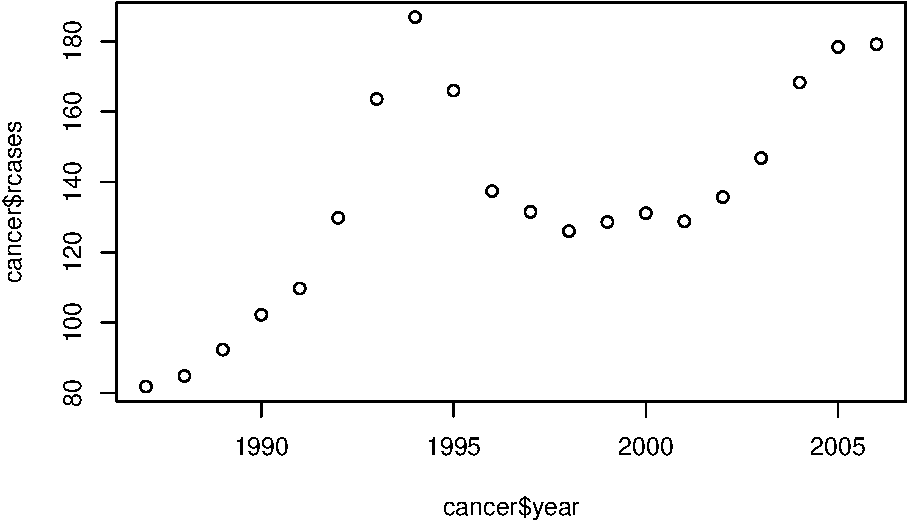
\includegraphics{phcm9795-R-notes_files/figure-latex/unnamed-chunk-49-1.pdf}

Let's define the plot to be joined by lines (\texttt{type="l"}), in the colour red (\texttt{col="red"}), providing meaningful labels for the x-axis and y-axis, and changing the scale of the y-axis to be between 0 and 200 (\texttt{ylim=c(0,200)}):

\begin{Shaded}
\begin{Highlighting}[]
\FunctionTok{plot}\NormalTok{(}\AttributeTok{x=}\NormalTok{cancer}\SpecialCharTok{$}\NormalTok{year, }\AttributeTok{y=}\NormalTok{cancer}\SpecialCharTok{$}\NormalTok{rcases, }
     \AttributeTok{type=}\StringTok{"l"}\NormalTok{, }\AttributeTok{col =} \StringTok{"red"}\NormalTok{, }
     \AttributeTok{xlab =} \StringTok{"Year"}\NormalTok{, }
     \AttributeTok{ylab =} \StringTok{"Age{-}standardised rate (per 100,000)"}\NormalTok{, }\AttributeTok{ylim=}\FunctionTok{c}\NormalTok{(}\DecValTok{0}\NormalTok{,}\DecValTok{200}\NormalTok{))}
\end{Highlighting}
\end{Shaded}

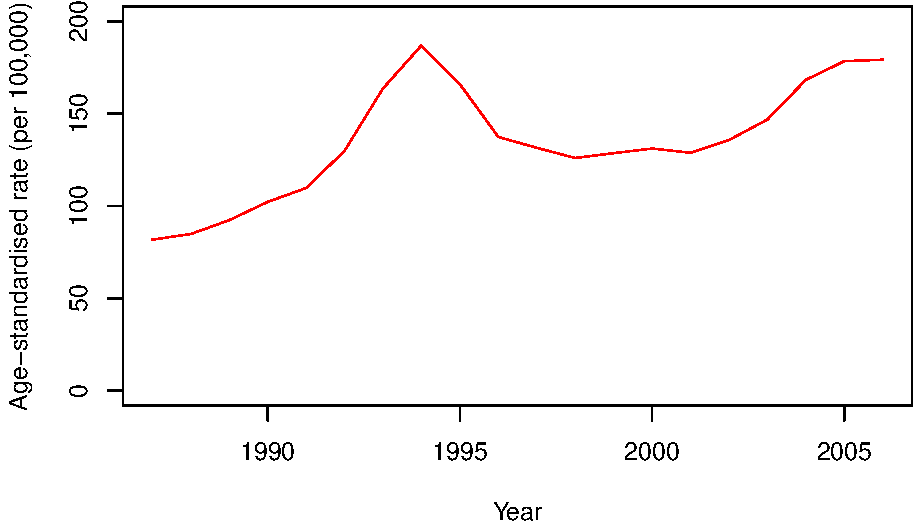
\includegraphics{phcm9795-R-notes_files/figure-latex/unnamed-chunk-50-1.pdf}

We can now add a second line to the plot using the \texttt{lines()} function, specifying a dashed line (\texttt{lty=2}), and add a legend to the plot:

\begin{Shaded}
\begin{Highlighting}[]
\FunctionTok{plot}\NormalTok{(}\AttributeTok{x=}\NormalTok{cancer}\SpecialCharTok{$}\NormalTok{year, }\AttributeTok{y=}\NormalTok{cancer}\SpecialCharTok{$}\NormalTok{rcases, }\AttributeTok{type=}\StringTok{"l"}\NormalTok{, }\AttributeTok{col =} \StringTok{"red"}\NormalTok{, }
     \AttributeTok{xlab =} \StringTok{"Year"}\NormalTok{, }\AttributeTok{ylab =} \StringTok{"Age{-}standardised rate (per 100,000)"}\NormalTok{, }
     \AttributeTok{ylim=}\FunctionTok{c}\NormalTok{(}\DecValTok{0}\NormalTok{,}\DecValTok{200}\NormalTok{))}

\FunctionTok{lines}\NormalTok{(cancer}\SpecialCharTok{$}\NormalTok{year, cancer}\SpecialCharTok{$}\NormalTok{rdeaths, }\AttributeTok{col =} \StringTok{"blue"}\NormalTok{, }\AttributeTok{type =} \StringTok{"l"}\NormalTok{, }\AttributeTok{lty =} \DecValTok{2}\NormalTok{)}

\FunctionTok{legend}\NormalTok{(}\StringTok{"topleft"}\NormalTok{, }\AttributeTok{legend=}\FunctionTok{c}\NormalTok{(}\StringTok{"Incidence"}\NormalTok{, }\StringTok{"Deaths"}\NormalTok{), }
       \AttributeTok{col=}\FunctionTok{c}\NormalTok{(}\StringTok{"red"}\NormalTok{, }\StringTok{"blue"}\NormalTok{), }\AttributeTok{lty =} \DecValTok{1}\SpecialCharTok{:}\DecValTok{2}\NormalTok{)}
\end{Highlighting}
\end{Shaded}

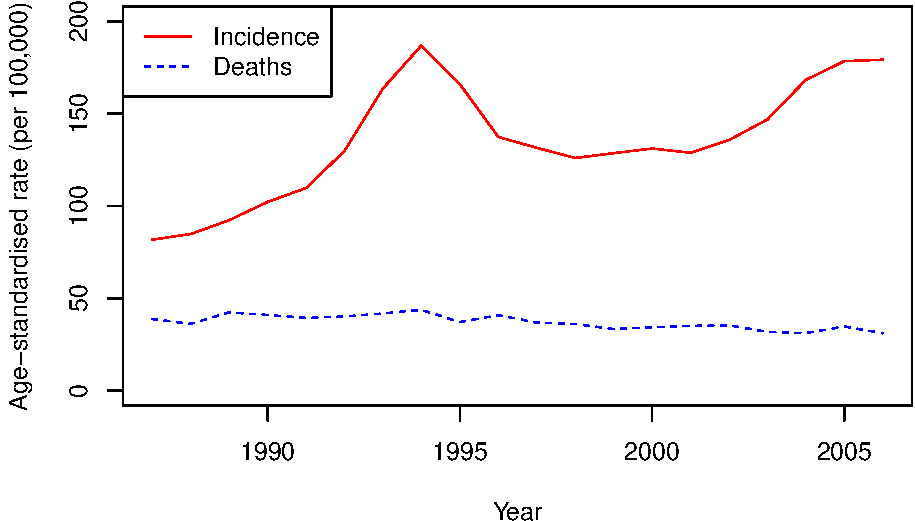
\includegraphics{phcm9795-R-notes_files/figure-latex/unnamed-chunk-51-1.pdf}

Note: coding for graphs is not always straightforward. Two excellent resources for creating graphs in R are: \href{https://r-graphics.org/}{R Graphics Cookbook} and \href{https://r-graph-gallery.com/}{The R Graph Gallery}.

\hypertarget{probability-and-probability-distributions}{%
\chapter{Probability and probability distributions}\label{probability-and-probability-distributions}}

\hypertarget{importing-data-into-r}{%
\section{Importing data into R}\label{importing-data-into-r}}

We have described previously how to import data that have been saved as R .rds files. It is quite common to have data saved in other file types, such as Microsoft Excel, or plain text files. In this section, we will demonstrate how to import data from other packages into R.

There are two useful packages for importing data into R: \texttt{haven} (for data that have been saved by Stata, SAS or SPSS) and \texttt{readxl} (for data saved by Microsoft Excel). Additionally, the \texttt{labelled} package is useful in working with data that have been labelled in Stata.

\hypertarget{importing-plain-text-data-into-r}{%
\subsection{Importing plain text data into R}\label{importing-plain-text-data-into-r}}

A \texttt{csv} file, or a ``comma separated variables'' file is commonly used to store data. These files have a very simple structure: they are plain text files, where data are separated by commas. csv files have the advantage that, as they are plain text files, they can be opened by a large number of programs (such as Notepad in Windows, TextEdit in MacOS, Microsoft Excel - even Microsoft Word). While they can be opened by Microsoft Excel, they can be opened by many other programs: the csv file can be thought of as the lingua-franca of data.

In this demonstration, we will use data on the weight of 1000 people entered in a csv file called \texttt{weight\_s2.csv} available on Moodle.

To confirm that the file is readable by any text editor, here are the first ten lines of the file, opened in Notepad on Microsoft Windows, and TextEdit on MacOS.

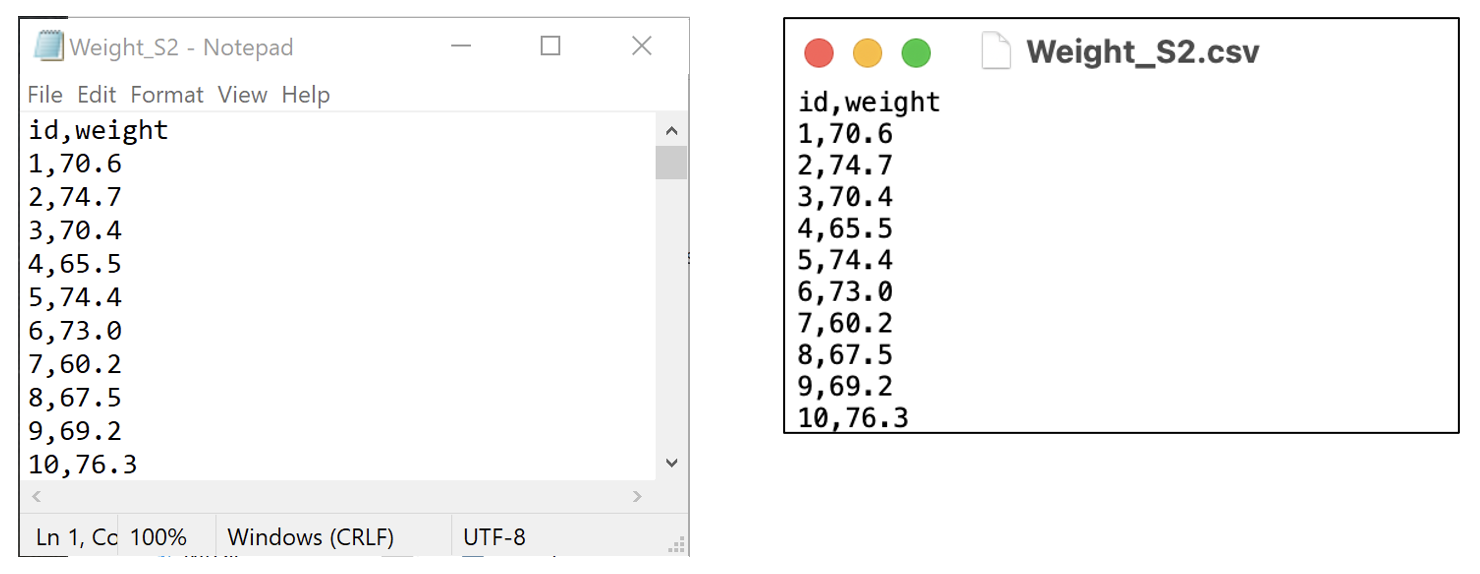
\includegraphics[width=0.66\linewidth]{img/mod02/import-01}

We can use the \texttt{read.csv} function:

\begin{Shaded}
\begin{Highlighting}[]
\NormalTok{sample }\OtherTok{\textless{}{-}} \FunctionTok{read.csv}\NormalTok{(}\StringTok{"data/examples/Weight\_s2.csv"}\NormalTok{)}
\end{Highlighting}
\end{Shaded}

Here, the \texttt{read.csv} function has the default that the first row of the dataset contains the variable names. If your data do not have column names, you can use \texttt{header=FALSE} in the function.

Note: there is an alternative function \texttt{read\_csv} which is part of the \texttt{readr} package (a component of the \texttt{tidyverse}). Some would argue that the \texttt{read\_csv} function is more appropriate to use because of an issue known as \texttt{strings.as.factors}. The \texttt{strings.as.factors} default was removed in R Version 4.0.0, so it is less important which of the two functions you use to import a \texttt{.csv} file. More information about this issue can be found \href{https://simplystatistics.org/posts/2015-07-24-stringsasfactors-an-unauthorized-biography}{here} and \href{https://developer.r-project.org/Blog/public/2020/02/16/stringsasfactors/}{here}.

\hypertarget{checking-your-data-for-errors-in-r}{%
\section{Checking your data for errors in R}\label{checking-your-data-for-errors-in-r}}

Before you start describing and analysing your data, it is important to make sure that no errors have been made during the data entry process. Basically, you are looking for values that are outside the range of possible or plausible values for that variable.

If an error is found, the best method for correcting the error is to go back to the original data e.g.~the hard copy questionnaire, to obtain the original value, entering the correct value into R If the original data is not available or the original data is also incorrect, the erroneous value is often excluded from the dataset.

For continuous variables, the easiest methods are to examine a boxplot and histogram. For example, a boxplot and histogram for the weight variable we just imported appear as:

\begin{Shaded}
\begin{Highlighting}[]
\FunctionTok{hist}\NormalTok{(sample}\SpecialCharTok{$}\NormalTok{weight, }\AttributeTok{xlab=}\StringTok{"Weight (kg)"}\NormalTok{, }\AttributeTok{main=}\StringTok{"Histogram of 1000 weights"}\NormalTok{)}
\end{Highlighting}
\end{Shaded}

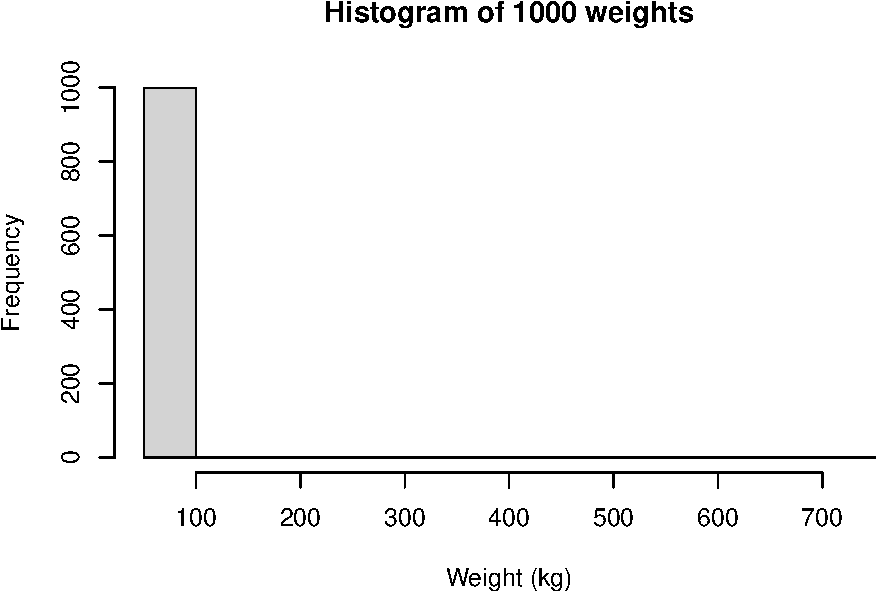
\includegraphics{phcm9795-R-notes_files/figure-latex/unnamed-chunk-54-1.pdf}

\begin{Shaded}
\begin{Highlighting}[]
\FunctionTok{boxplot}\NormalTok{(sample}\SpecialCharTok{$}\NormalTok{weight, }\AttributeTok{xlab=}\StringTok{"Weight (kg)"}\NormalTok{, }\AttributeTok{main=}\StringTok{"Boxplot of 1000 weights"}\NormalTok{)}
\end{Highlighting}
\end{Shaded}

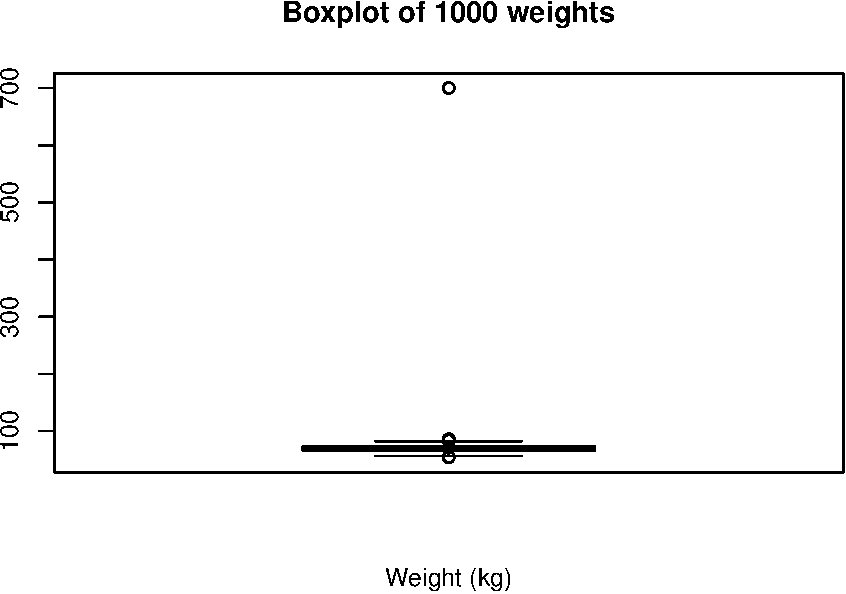
\includegraphics{phcm9795-R-notes_files/figure-latex/unnamed-chunk-54-2.pdf}

There is a clear outlying point shown in the boxplot. Although not obvious, the same point is shown in the histogram as a bar around 700 with a very short height.

We can identify any outlying observations in the dataset using the \texttt{subset} function. You will need to decide if these values are a data entry error or are biologically plausible. If an extreme value or ``outlier'', is biologically plausible, it should be included in all analyses.

For example, to list any observations from the \texttt{sample} dataset with a weight larger than 200:

\begin{Shaded}
\begin{Highlighting}[]
\FunctionTok{subset}\NormalTok{(sample, weight}\SpecialCharTok{\textgreater{}}\DecValTok{200}\NormalTok{)}
\end{Highlighting}
\end{Shaded}

 
  \providecommand{\huxb}[2]{\arrayrulecolor[RGB]{#1}\global\arrayrulewidth=#2pt}
  \providecommand{\huxvb}[2]{\color[RGB]{#1}\vrule width #2pt}
  \providecommand{\huxtpad}[1]{\rule{0pt}{#1}}
  \providecommand{\huxbpad}[1]{\rule[-#1]{0pt}{#1}}

\begin{table}[ht]
\begin{centerbox}
\begin{threeparttable}
\captionsetup{justification=centering,singlelinecheck=off}
\caption{\label{tab:unnamed-chunk-55} }
 \setlength{\tabcolsep}{0pt}
\begin{tabular}{l l}


\hhline{>{\huxb{0, 0, 0}{0.4}}->{\huxb{0, 0, 0}{0.4}}-}
\arrayrulecolor{black}

\multicolumn{1}{!{\huxvb{0, 0, 0}{0.4}}r!{\huxvb{0, 0, 0}{0}}}{\huxtpad{6pt + 1em}\raggedleft \hspace{6pt} \textbf{id} \hspace{6pt}\huxbpad{6pt}} &
\multicolumn{1}{r!{\huxvb{0, 0, 0}{0.4}}}{\huxtpad{6pt + 1em}\raggedleft \hspace{6pt} \textbf{weight} \hspace{6pt}\huxbpad{6pt}} \tabularnewline[-0.5pt]


\hhline{>{\huxb{0, 0, 0}{0.4}}->{\huxb{0, 0, 0}{0.4}}-}
\arrayrulecolor{black}

\multicolumn{1}{!{\huxvb{0, 0, 0}{0.4}}r!{\huxvb{0, 0, 0}{0}}}{\cellcolor[RGB]{242, 242, 242}\huxtpad{6pt + 1em}\raggedleft \hspace{6pt} 58 \hspace{6pt}\huxbpad{6pt}} &
\multicolumn{1}{r!{\huxvb{0, 0, 0}{0.4}}}{\cellcolor[RGB]{242, 242, 242}\huxtpad{6pt + 1em}\raggedleft \hspace{6pt} 700 \hspace{6pt}\huxbpad{6pt}} \tabularnewline[-0.5pt]


\hhline{>{\huxb{0, 0, 0}{0.4}}->{\huxb{0, 0, 0}{0.4}}-}
\arrayrulecolor{black}
\end{tabular}
\end{threeparttable}\par\end{centerbox}

\end{table}
 

We see that there is a very high value of 700.2kg. A value as high as 700kg is likely to be a data entry error (e.g.~error in entering an extra zero) and is not a plausible weight value. Here, \textbf{you should check your original data}.

You might find that the original weight was recorded in medical records as 70.2kg. You can change this in R by writing code.

\textbf{Note:} many statistical packages will allow you to view a spreadsheet version of your data and edit values in that spreadsheet. This is not best practice, as corrected observations may revert to their original values depending on whether the edited data have been saved or not. By using code-based recoding, the changes will be reproduced the next time the code is run.

We will use an \texttt{ifelse} statement to recode the incorrect weight of 700.2kg into 70.2kg. The form of the \texttt{ifelse} statement is as follows:

\texttt{ifelse(test,\ value\_if\_true,\ value\_if\_false)}

Our code will create a new column (called \texttt{weight\_clean}) in the \texttt{sample} dataframe. We will test whether \texttt{weight} is equal to 700.2; if this is true, we will assign \texttt{weight\_clean} to be 70.2, otherwise \texttt{weight\_clean} will equal the value of \texttt{weight}.

Putting it all together:

\begin{Shaded}
\begin{Highlighting}[]
\NormalTok{sample}\SpecialCharTok{$}\NormalTok{weight\_clean }\OtherTok{=} \FunctionTok{ifelse}\NormalTok{(sample}\SpecialCharTok{$}\NormalTok{weight}\SpecialCharTok{==}\FloatTok{700.2}\NormalTok{, }\FloatTok{70.2}\NormalTok{, sample}\SpecialCharTok{$}\NormalTok{weight)}
\end{Highlighting}
\end{Shaded}

\textbf{Note:} if an extreme value lies within the range of biological plausibility it should not be removed from analysis.

Once you have checked your data for errors, you are ready to start analysing your data.

\hypertarget{what-on-earth}{%
\subsection{What on earth: == ?}\label{what-on-earth}}

In R, the test of equality is denoted by two equal signs: \texttt{==}. So we would use \texttt{==} to test whether an observation is equal to a certain value. Let's see an example:

\begin{Shaded}
\begin{Highlighting}[]
\CommentTok{\# Test whether 6 is equal to 6}
\DecValTok{6} \SpecialCharTok{==} \DecValTok{6}
\end{Highlighting}
\end{Shaded}

\begin{verbatim}
## [1] TRUE
\end{verbatim}

\begin{Shaded}
\begin{Highlighting}[]
\CommentTok{\# Test whether 6 is equal to 42}
\DecValTok{6} \SpecialCharTok{==} \DecValTok{42}
\end{Highlighting}
\end{Shaded}

\begin{verbatim}
## [1] FALSE
\end{verbatim}

You can read the \texttt{==} as ``is equal to''. So the code \texttt{sample\$weight\ ==\ 700.2} is read as: ``is the value of weight from the data frame sample equal to 700.2?''. In our \texttt{ifelse} statement above, if this condition is true, we replace \texttt{weight} by 70.2; if it is false, we leave weight as is.

\hypertarget{overlaying-a-normal-curve-on-a-histogram}{%
\section{Overlaying a Normal curve on a histogram}\label{overlaying-a-normal-curve-on-a-histogram}}

It can be useful to produce a histogram with an overlayed Normal curve to assess whether our sample appears approximately Normally distributed. We can do this by plotting a histogram using the \texttt{hist()} function. As we're overlaying a probability distribution, we request the histogram be plotted on a probability scale, rather than a frequency scale, using \texttt{probability=TRUE}.

We then request a curve be overlayed using the \texttt{curve()} function:

\begin{itemize}
\item
  the curve should be based on the Normal distribution (\texttt{dnorm});

  \begin{itemize}
  \item
    with a mean equal to the mean of the cleaned weight: \texttt{mean(sample\$weight\_clean));}
  \item
    and a standard deviation equal to the standard deviation of the cleaned weight: \texttt{sd(sample\$weight\_clean))}
  \end{itemize}
\item
  using a dark-blue colour;
\item
  and added to the previous histogram (rather than plotting the curve by itself): \texttt{add=TRUE}
\end{itemize}

\begin{Shaded}
\begin{Highlighting}[]
\FunctionTok{hist}\NormalTok{(sample}\SpecialCharTok{$}\NormalTok{weight\_clean,}
     \AttributeTok{xlab=}\StringTok{"Weight (kg)"}\NormalTok{,}
     \AttributeTok{main=}\StringTok{"Histogram of 1000 weights"}\NormalTok{,}
     \AttributeTok{probability =} \ConstantTok{TRUE}\NormalTok{)}

\FunctionTok{curve}\NormalTok{(}\FunctionTok{dnorm}\NormalTok{(x,}
            \AttributeTok{mean=}\FunctionTok{mean}\NormalTok{(sample}\SpecialCharTok{$}\NormalTok{weight\_clean),}
            \AttributeTok{sd=}\FunctionTok{sd}\NormalTok{(sample}\SpecialCharTok{$}\NormalTok{weight\_clean)),}
      \AttributeTok{col=}\StringTok{"darkblue"}\NormalTok{,}
      \AttributeTok{add=}\ConstantTok{TRUE}\NormalTok{)}
\end{Highlighting}
\end{Shaded}

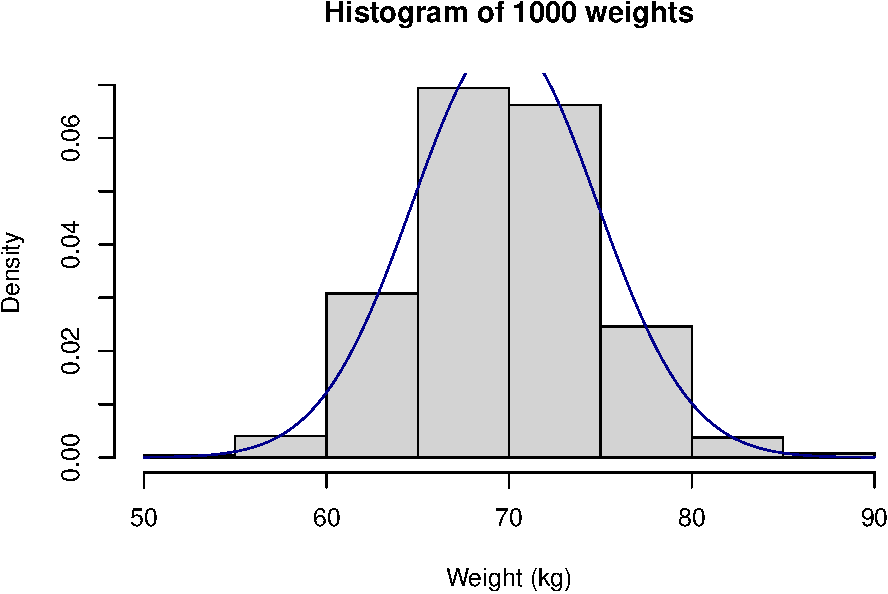
\includegraphics{phcm9795-R-notes_files/figure-latex/unnamed-chunk-58-1.pdf}

Notice that the top of the curve is chopped off. We can plot the whole curve by extending the y-axis of the histogram to 0.1:

\begin{Shaded}
\begin{Highlighting}[]
\FunctionTok{hist}\NormalTok{(sample}\SpecialCharTok{$}\NormalTok{weight\_clean, }
     \AttributeTok{xlab=}\StringTok{"Weight (kg)"}\NormalTok{,}
     \AttributeTok{main=}\StringTok{"Histogram of 1000 weights"}\NormalTok{,}
     \AttributeTok{probability =} \ConstantTok{TRUE}\NormalTok{,}
     \AttributeTok{ylim=}\FunctionTok{c}\NormalTok{(}\DecValTok{0}\NormalTok{,}\FloatTok{0.1}\NormalTok{))}

\FunctionTok{curve}\NormalTok{(}\FunctionTok{dnorm}\NormalTok{(x,}
            \AttributeTok{mean=}\FunctionTok{mean}\NormalTok{(sample}\SpecialCharTok{$}\NormalTok{weight\_clean),}
            \AttributeTok{sd=}\FunctionTok{sd}\NormalTok{(sample}\SpecialCharTok{$}\NormalTok{weight\_clean)),}
      \AttributeTok{col=}\StringTok{"darkblue"}\NormalTok{,}
      \AttributeTok{add=}\ConstantTok{TRUE}\NormalTok{)}
\end{Highlighting}
\end{Shaded}

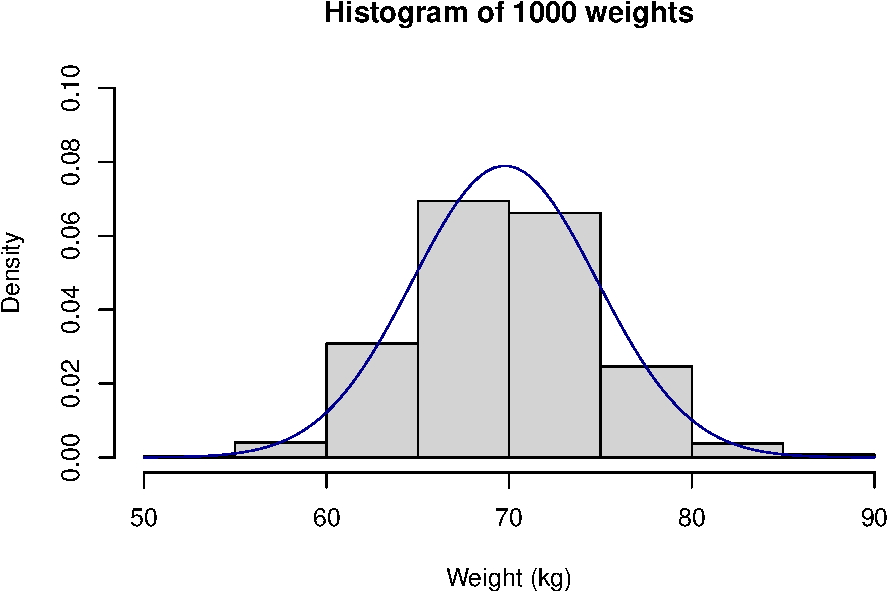
\includegraphics{phcm9795-R-notes_files/figure-latex/unnamed-chunk-59-1.pdf}

\hypertarget{descriptive-statistics-for-checking-normality}{%
\section{Descriptive statistics for checking normality}\label{descriptive-statistics-for-checking-normality}}

All the descriptive statistics including \emph{skewness} and \emph{kurtosis} discussed in this module can be obtained using the \texttt{descriptives} function from the \texttt{jmv} package. In particular, skewness and kurtosis can be requested in addition to the default statistics by including: \texttt{skew=TRUE,\ kurt=TRUE}:

\begin{Shaded}
\begin{Highlighting}[]
\FunctionTok{library}\NormalTok{(jmv)}

\FunctionTok{descriptives}\NormalTok{(}\AttributeTok{data=}\NormalTok{sample, }\AttributeTok{vars=}\NormalTok{weight\_clean, }\AttributeTok{skew=}\ConstantTok{TRUE}\NormalTok{, }\AttributeTok{kurt=}\ConstantTok{TRUE}\NormalTok{)}
\end{Highlighting}
\end{Shaded}

\begin{verbatim}
## 
##  DESCRIPTIVES
## 
##  Descriptives                            
##  ─────────────────────────────────────── 
##                           weight_clean   
##  ─────────────────────────────────────── 
##    N                              1000   
##    Missing                           0   
##    Mean                       69.76450   
##    Median                     69.80000   
##    Standard deviation         5.052676   
##    Minimum                    53.80000   
##    Maximum                    85.80000   
##    Skewness                 0.07360659   
##    Std. error skewness      0.07734382   
##    Kurtosis                 0.05418774   
##    Std. error kurtosis       0.1545343   
##  ───────────────────────────────────────
\end{verbatim}

\hypertarget{import-excel}{%
\section{Importing Excel data into R}\label{import-excel}}

Another common type of file that data are stored in is a Microsoft Excel file (.xls or .xlsx). In this demonstration, we will import a selection of records from a large health survey, stored in the file \texttt{health-survey.xlsx}.

The health survey data contains 1140 records, comprising:

\begin{itemize}
\tightlist
\item
  sex: 1 = respondent identifies as male; 2 = respondent identifies as female
\item
  height: height in meters
\item
  weight: weight in kilograms
\end{itemize}

To import data from Microsoft Excel, we can use the \texttt{read\_excel()} function in the \texttt{readxl} package.

\begin{Shaded}
\begin{Highlighting}[]
\FunctionTok{library}\NormalTok{(readxl)}

\NormalTok{survey }\OtherTok{\textless{}{-}} \FunctionTok{read\_excel}\NormalTok{(}\StringTok{"data/examples/health{-}survey.xlsx"}\NormalTok{)}
\FunctionTok{summary}\NormalTok{(survey)}
\end{Highlighting}
\end{Shaded}

\begin{verbatim}
##       sex           height          weight      
##  Min.   :1.00   Min.   :1.220   Min.   : 22.70  
##  1st Qu.:1.00   1st Qu.:1.630   1st Qu.: 68.00  
##  Median :2.00   Median :1.700   Median : 79.40  
##  Mean   :1.55   Mean   :1.698   Mean   : 81.19  
##  3rd Qu.:2.00   3rd Qu.:1.780   3rd Qu.: 90.70  
##  Max.   :2.00   Max.   :2.010   Max.   :213.20
\end{verbatim}

We can see that sex has been entered as a numeric variable. We should transform it into a factor so that we can assign labels to each category:

\begin{Shaded}
\begin{Highlighting}[]
\NormalTok{survey}\SpecialCharTok{$}\NormalTok{sex }\OtherTok{\textless{}{-}} \FunctionTok{factor}\NormalTok{(survey}\SpecialCharTok{$}\NormalTok{sex, }\AttributeTok{level=}\FunctionTok{c}\NormalTok{(}\DecValTok{1}\NormalTok{,}\DecValTok{2}\NormalTok{), }\AttributeTok{labels=}\FunctionTok{c}\NormalTok{(}\StringTok{"Male"}\NormalTok{, }\StringTok{"Female"}\NormalTok{))}

\FunctionTok{summary}\NormalTok{(survey}\SpecialCharTok{$}\NormalTok{sex)}
\end{Highlighting}
\end{Shaded}

\begin{verbatim}
##   Male Female 
##    513    627
\end{verbatim}

We also note that height looks like it has been entered as meters, and weight as kilograms.

\hypertarget{generating-new-variables}{%
\section{Generating new variables}\label{generating-new-variables}}

Our health survey data contains information on height and weight. We often summarise body size using BMI: body mass index which is calculated as: \(\frac{\text{weight (kg)}}{(\text{height (m)})^2}\)

We can create a new column in our data frame in many ways, such as using the following approach:

\texttt{dataframe\$new\_column\ \textless{}-\ \textless{}formula\textgreater{}}

For example:

\begin{Shaded}
\begin{Highlighting}[]
\NormalTok{survey}\SpecialCharTok{$}\NormalTok{bmi }\OtherTok{\textless{}{-}}\NormalTok{ survey}\SpecialCharTok{$}\NormalTok{weight }\SpecialCharTok{/}\NormalTok{ (survey}\SpecialCharTok{$}\NormalTok{height}\SpecialCharTok{\^{}}\DecValTok{2}\NormalTok{)}
\end{Highlighting}
\end{Shaded}

We should check the construction of the new variable by examining some records. The \texttt{head()} and \texttt{tail()} functions list the first and last 6 records in any dataset. We can also examine a histogram and boxplot:

\begin{Shaded}
\begin{Highlighting}[]
\FunctionTok{head}\NormalTok{(survey)}
\end{Highlighting}
\end{Shaded}

 
  \providecommand{\huxb}[2]{\arrayrulecolor[RGB]{#1}\global\arrayrulewidth=#2pt}
  \providecommand{\huxvb}[2]{\color[RGB]{#1}\vrule width #2pt}
  \providecommand{\huxtpad}[1]{\rule{0pt}{#1}}
  \providecommand{\huxbpad}[1]{\rule[-#1]{0pt}{#1}}

\begin{table}[ht]
\begin{centerbox}
\begin{threeparttable}
\captionsetup{justification=centering,singlelinecheck=off}
\caption{\label{tab:unnamed-chunk-64} }
 \setlength{\tabcolsep}{0pt}
\begin{tabular}{l l l l}


\hhline{>{\huxb{0, 0, 0}{0.4}}->{\huxb{0, 0, 0}{0.4}}->{\huxb{0, 0, 0}{0.4}}->{\huxb{0, 0, 0}{0.4}}-}
\arrayrulecolor{black}

\multicolumn{1}{!{\huxvb{0, 0, 0}{0.4}}l!{\huxvb{0, 0, 0}{0}}}{\huxtpad{6pt + 1em}\raggedright \hspace{6pt} \textbf{sex} \hspace{6pt}\huxbpad{6pt}} &
\multicolumn{1}{r!{\huxvb{0, 0, 0}{0}}}{\huxtpad{6pt + 1em}\raggedleft \hspace{6pt} \textbf{height} \hspace{6pt}\huxbpad{6pt}} &
\multicolumn{1}{r!{\huxvb{0, 0, 0}{0}}}{\huxtpad{6pt + 1em}\raggedleft \hspace{6pt} \textbf{weight} \hspace{6pt}\huxbpad{6pt}} &
\multicolumn{1}{r!{\huxvb{0, 0, 0}{0.4}}}{\huxtpad{6pt + 1em}\raggedleft \hspace{6pt} \textbf{bmi} \hspace{6pt}\huxbpad{6pt}} \tabularnewline[-0.5pt]


\hhline{>{\huxb{0, 0, 0}{0.4}}->{\huxb{0, 0, 0}{0.4}}->{\huxb{0, 0, 0}{0.4}}->{\huxb{0, 0, 0}{0.4}}-}
\arrayrulecolor{black}

\multicolumn{1}{!{\huxvb{0, 0, 0}{0.4}}l!{\huxvb{0, 0, 0}{0}}}{\cellcolor[RGB]{242, 242, 242}\huxtpad{6pt + 1em}\raggedright \hspace{6pt} Male \hspace{6pt}\huxbpad{6pt}} &
\multicolumn{1}{r!{\huxvb{0, 0, 0}{0}}}{\cellcolor[RGB]{242, 242, 242}\huxtpad{6pt + 1em}\raggedleft \hspace{6pt} 1.63 \hspace{6pt}\huxbpad{6pt}} &
\multicolumn{1}{r!{\huxvb{0, 0, 0}{0}}}{\cellcolor[RGB]{242, 242, 242}\huxtpad{6pt + 1em}\raggedleft \hspace{6pt} 81.7 \hspace{6pt}\huxbpad{6pt}} &
\multicolumn{1}{r!{\huxvb{0, 0, 0}{0.4}}}{\cellcolor[RGB]{242, 242, 242}\huxtpad{6pt + 1em}\raggedleft \hspace{6pt} 30.8 \hspace{6pt}\huxbpad{6pt}} \tabularnewline[-0.5pt]


\hhline{>{\huxb{0, 0, 0}{0.4}}|>{\huxb{0, 0, 0}{0.4}}|}
\arrayrulecolor{black}

\multicolumn{1}{!{\huxvb{0, 0, 0}{0.4}}l!{\huxvb{0, 0, 0}{0}}}{\huxtpad{6pt + 1em}\raggedright \hspace{6pt} Male \hspace{6pt}\huxbpad{6pt}} &
\multicolumn{1}{r!{\huxvb{0, 0, 0}{0}}}{\huxtpad{6pt + 1em}\raggedleft \hspace{6pt} 1.63 \hspace{6pt}\huxbpad{6pt}} &
\multicolumn{1}{r!{\huxvb{0, 0, 0}{0}}}{\huxtpad{6pt + 1em}\raggedleft \hspace{6pt} 68\hphantom{0}\hphantom{0} \hspace{6pt}\huxbpad{6pt}} &
\multicolumn{1}{r!{\huxvb{0, 0, 0}{0.4}}}{\huxtpad{6pt + 1em}\raggedleft \hspace{6pt} 25.6 \hspace{6pt}\huxbpad{6pt}} \tabularnewline[-0.5pt]


\hhline{>{\huxb{0, 0, 0}{0.4}}|>{\huxb{0, 0, 0}{0.4}}|}
\arrayrulecolor{black}

\multicolumn{1}{!{\huxvb{0, 0, 0}{0.4}}l!{\huxvb{0, 0, 0}{0}}}{\cellcolor[RGB]{242, 242, 242}\huxtpad{6pt + 1em}\raggedright \hspace{6pt} Male \hspace{6pt}\huxbpad{6pt}} &
\multicolumn{1}{r!{\huxvb{0, 0, 0}{0}}}{\cellcolor[RGB]{242, 242, 242}\huxtpad{6pt + 1em}\raggedleft \hspace{6pt} 1.85 \hspace{6pt}\huxbpad{6pt}} &
\multicolumn{1}{r!{\huxvb{0, 0, 0}{0}}}{\cellcolor[RGB]{242, 242, 242}\huxtpad{6pt + 1em}\raggedleft \hspace{6pt} 97.1 \hspace{6pt}\huxbpad{6pt}} &
\multicolumn{1}{r!{\huxvb{0, 0, 0}{0.4}}}{\cellcolor[RGB]{242, 242, 242}\huxtpad{6pt + 1em}\raggedleft \hspace{6pt} 28.4 \hspace{6pt}\huxbpad{6pt}} \tabularnewline[-0.5pt]


\hhline{>{\huxb{0, 0, 0}{0.4}}|>{\huxb{0, 0, 0}{0.4}}|}
\arrayrulecolor{black}

\multicolumn{1}{!{\huxvb{0, 0, 0}{0.4}}l!{\huxvb{0, 0, 0}{0}}}{\huxtpad{6pt + 1em}\raggedright \hspace{6pt} Male \hspace{6pt}\huxbpad{6pt}} &
\multicolumn{1}{r!{\huxvb{0, 0, 0}{0}}}{\huxtpad{6pt + 1em}\raggedleft \hspace{6pt} 1.78 \hspace{6pt}\huxbpad{6pt}} &
\multicolumn{1}{r!{\huxvb{0, 0, 0}{0}}}{\huxtpad{6pt + 1em}\raggedleft \hspace{6pt} 89.8 \hspace{6pt}\huxbpad{6pt}} &
\multicolumn{1}{r!{\huxvb{0, 0, 0}{0.4}}}{\huxtpad{6pt + 1em}\raggedleft \hspace{6pt} 28.3 \hspace{6pt}\huxbpad{6pt}} \tabularnewline[-0.5pt]


\hhline{>{\huxb{0, 0, 0}{0.4}}|>{\huxb{0, 0, 0}{0.4}}|}
\arrayrulecolor{black}

\multicolumn{1}{!{\huxvb{0, 0, 0}{0.4}}l!{\huxvb{0, 0, 0}{0}}}{\cellcolor[RGB]{242, 242, 242}\huxtpad{6pt + 1em}\raggedright \hspace{6pt} Male \hspace{6pt}\huxbpad{6pt}} &
\multicolumn{1}{r!{\huxvb{0, 0, 0}{0}}}{\cellcolor[RGB]{242, 242, 242}\huxtpad{6pt + 1em}\raggedleft \hspace{6pt} 1.73 \hspace{6pt}\huxbpad{6pt}} &
\multicolumn{1}{r!{\huxvb{0, 0, 0}{0}}}{\cellcolor[RGB]{242, 242, 242}\huxtpad{6pt + 1em}\raggedleft \hspace{6pt} 70.3 \hspace{6pt}\huxbpad{6pt}} &
\multicolumn{1}{r!{\huxvb{0, 0, 0}{0.4}}}{\cellcolor[RGB]{242, 242, 242}\huxtpad{6pt + 1em}\raggedleft \hspace{6pt} 23.5 \hspace{6pt}\huxbpad{6pt}} \tabularnewline[-0.5pt]


\hhline{>{\huxb{0, 0, 0}{0.4}}|>{\huxb{0, 0, 0}{0.4}}|}
\arrayrulecolor{black}

\multicolumn{1}{!{\huxvb{0, 0, 0}{0.4}}l!{\huxvb{0, 0, 0}{0}}}{\huxtpad{6pt + 1em}\raggedright \hspace{6pt} Female \hspace{6pt}\huxbpad{6pt}} &
\multicolumn{1}{r!{\huxvb{0, 0, 0}{0}}}{\huxtpad{6pt + 1em}\raggedleft \hspace{6pt} 1.57 \hspace{6pt}\huxbpad{6pt}} &
\multicolumn{1}{r!{\huxvb{0, 0, 0}{0}}}{\huxtpad{6pt + 1em}\raggedleft \hspace{6pt} 85.7 \hspace{6pt}\huxbpad{6pt}} &
\multicolumn{1}{r!{\huxvb{0, 0, 0}{0.4}}}{\huxtpad{6pt + 1em}\raggedleft \hspace{6pt} 34.8 \hspace{6pt}\huxbpad{6pt}} \tabularnewline[-0.5pt]


\hhline{>{\huxb{0, 0, 0}{0.4}}->{\huxb{0, 0, 0}{0.4}}->{\huxb{0, 0, 0}{0.4}}->{\huxb{0, 0, 0}{0.4}}-}
\arrayrulecolor{black}
\end{tabular}
\end{threeparttable}\par\end{centerbox}

\end{table}
 

\begin{Shaded}
\begin{Highlighting}[]
\FunctionTok{tail}\NormalTok{(survey)}
\end{Highlighting}
\end{Shaded}

 
  \providecommand{\huxb}[2]{\arrayrulecolor[RGB]{#1}\global\arrayrulewidth=#2pt}
  \providecommand{\huxvb}[2]{\color[RGB]{#1}\vrule width #2pt}
  \providecommand{\huxtpad}[1]{\rule{0pt}{#1}}
  \providecommand{\huxbpad}[1]{\rule[-#1]{0pt}{#1}}

\begin{table}[ht]
\begin{centerbox}
\begin{threeparttable}
\captionsetup{justification=centering,singlelinecheck=off}
\caption{\label{tab:unnamed-chunk-64} }
 \setlength{\tabcolsep}{0pt}
\begin{tabular}{l l l l}


\hhline{>{\huxb{0, 0, 0}{0.4}}->{\huxb{0, 0, 0}{0.4}}->{\huxb{0, 0, 0}{0.4}}->{\huxb{0, 0, 0}{0.4}}-}
\arrayrulecolor{black}

\multicolumn{1}{!{\huxvb{0, 0, 0}{0.4}}l!{\huxvb{0, 0, 0}{0}}}{\huxtpad{6pt + 1em}\raggedright \hspace{6pt} \textbf{sex} \hspace{6pt}\huxbpad{6pt}} &
\multicolumn{1}{r!{\huxvb{0, 0, 0}{0}}}{\huxtpad{6pt + 1em}\raggedleft \hspace{6pt} \textbf{height} \hspace{6pt}\huxbpad{6pt}} &
\multicolumn{1}{r!{\huxvb{0, 0, 0}{0}}}{\huxtpad{6pt + 1em}\raggedleft \hspace{6pt} \textbf{weight} \hspace{6pt}\huxbpad{6pt}} &
\multicolumn{1}{r!{\huxvb{0, 0, 0}{0.4}}}{\huxtpad{6pt + 1em}\raggedleft \hspace{6pt} \textbf{bmi} \hspace{6pt}\huxbpad{6pt}} \tabularnewline[-0.5pt]


\hhline{>{\huxb{0, 0, 0}{0.4}}->{\huxb{0, 0, 0}{0.4}}->{\huxb{0, 0, 0}{0.4}}->{\huxb{0, 0, 0}{0.4}}-}
\arrayrulecolor{black}

\multicolumn{1}{!{\huxvb{0, 0, 0}{0.4}}l!{\huxvb{0, 0, 0}{0}}}{\cellcolor[RGB]{242, 242, 242}\huxtpad{6pt + 1em}\raggedright \hspace{6pt} Female \hspace{6pt}\huxbpad{6pt}} &
\multicolumn{1}{r!{\huxvb{0, 0, 0}{0}}}{\cellcolor[RGB]{242, 242, 242}\huxtpad{6pt + 1em}\raggedleft \hspace{6pt} 1.65 \hspace{6pt}\huxbpad{6pt}} &
\multicolumn{1}{r!{\huxvb{0, 0, 0}{0}}}{\cellcolor[RGB]{242, 242, 242}\huxtpad{6pt + 1em}\raggedleft \hspace{6pt} 95.7 \hspace{6pt}\huxbpad{6pt}} &
\multicolumn{1}{r!{\huxvb{0, 0, 0}{0.4}}}{\cellcolor[RGB]{242, 242, 242}\huxtpad{6pt + 1em}\raggedleft \hspace{6pt} 35.2 \hspace{6pt}\huxbpad{6pt}} \tabularnewline[-0.5pt]


\hhline{>{\huxb{0, 0, 0}{0.4}}|>{\huxb{0, 0, 0}{0.4}}|}
\arrayrulecolor{black}

\multicolumn{1}{!{\huxvb{0, 0, 0}{0.4}}l!{\huxvb{0, 0, 0}{0}}}{\huxtpad{6pt + 1em}\raggedright \hspace{6pt} Male \hspace{6pt}\huxbpad{6pt}} &
\multicolumn{1}{r!{\huxvb{0, 0, 0}{0}}}{\huxtpad{6pt + 1em}\raggedleft \hspace{6pt} 1.8\hphantom{0} \hspace{6pt}\huxbpad{6pt}} &
\multicolumn{1}{r!{\huxvb{0, 0, 0}{0}}}{\huxtpad{6pt + 1em}\raggedleft \hspace{6pt} 79.4 \hspace{6pt}\huxbpad{6pt}} &
\multicolumn{1}{r!{\huxvb{0, 0, 0}{0.4}}}{\huxtpad{6pt + 1em}\raggedleft \hspace{6pt} 24.5 \hspace{6pt}\huxbpad{6pt}} \tabularnewline[-0.5pt]


\hhline{>{\huxb{0, 0, 0}{0.4}}|>{\huxb{0, 0, 0}{0.4}}|}
\arrayrulecolor{black}

\multicolumn{1}{!{\huxvb{0, 0, 0}{0.4}}l!{\huxvb{0, 0, 0}{0}}}{\cellcolor[RGB]{242, 242, 242}\huxtpad{6pt + 1em}\raggedright \hspace{6pt} Female \hspace{6pt}\huxbpad{6pt}} &
\multicolumn{1}{r!{\huxvb{0, 0, 0}{0}}}{\cellcolor[RGB]{242, 242, 242}\huxtpad{6pt + 1em}\raggedleft \hspace{6pt} 1.73 \hspace{6pt}\huxbpad{6pt}} &
\multicolumn{1}{r!{\huxvb{0, 0, 0}{0}}}{\cellcolor[RGB]{242, 242, 242}\huxtpad{6pt + 1em}\raggedleft \hspace{6pt} 83\hphantom{0}\hphantom{0} \hspace{6pt}\huxbpad{6pt}} &
\multicolumn{1}{r!{\huxvb{0, 0, 0}{0.4}}}{\cellcolor[RGB]{242, 242, 242}\huxtpad{6pt + 1em}\raggedleft \hspace{6pt} 27.7 \hspace{6pt}\huxbpad{6pt}} \tabularnewline[-0.5pt]


\hhline{>{\huxb{0, 0, 0}{0.4}}|>{\huxb{0, 0, 0}{0.4}}|}
\arrayrulecolor{black}

\multicolumn{1}{!{\huxvb{0, 0, 0}{0.4}}l!{\huxvb{0, 0, 0}{0}}}{\huxtpad{6pt + 1em}\raggedright \hspace{6pt} Female \hspace{6pt}\huxbpad{6pt}} &
\multicolumn{1}{r!{\huxvb{0, 0, 0}{0}}}{\huxtpad{6pt + 1em}\raggedleft \hspace{6pt} 1.57 \hspace{6pt}\huxbpad{6pt}} &
\multicolumn{1}{r!{\huxvb{0, 0, 0}{0}}}{\huxtpad{6pt + 1em}\raggedleft \hspace{6pt} 61.2 \hspace{6pt}\huxbpad{6pt}} &
\multicolumn{1}{r!{\huxvb{0, 0, 0}{0.4}}}{\huxtpad{6pt + 1em}\raggedleft \hspace{6pt} 24.8 \hspace{6pt}\huxbpad{6pt}} \tabularnewline[-0.5pt]


\hhline{>{\huxb{0, 0, 0}{0.4}}|>{\huxb{0, 0, 0}{0.4}}|}
\arrayrulecolor{black}

\multicolumn{1}{!{\huxvb{0, 0, 0}{0.4}}l!{\huxvb{0, 0, 0}{0}}}{\cellcolor[RGB]{242, 242, 242}\huxtpad{6pt + 1em}\raggedright \hspace{6pt} Male \hspace{6pt}\huxbpad{6pt}} &
\multicolumn{1}{r!{\huxvb{0, 0, 0}{0}}}{\cellcolor[RGB]{242, 242, 242}\huxtpad{6pt + 1em}\raggedleft \hspace{6pt} 1.7\hphantom{0} \hspace{6pt}\huxbpad{6pt}} &
\multicolumn{1}{r!{\huxvb{0, 0, 0}{0}}}{\cellcolor[RGB]{242, 242, 242}\huxtpad{6pt + 1em}\raggedleft \hspace{6pt} 73\hphantom{0}\hphantom{0} \hspace{6pt}\huxbpad{6pt}} &
\multicolumn{1}{r!{\huxvb{0, 0, 0}{0.4}}}{\cellcolor[RGB]{242, 242, 242}\huxtpad{6pt + 1em}\raggedleft \hspace{6pt} 25.3 \hspace{6pt}\huxbpad{6pt}} \tabularnewline[-0.5pt]


\hhline{>{\huxb{0, 0, 0}{0.4}}|>{\huxb{0, 0, 0}{0.4}}|}
\arrayrulecolor{black}

\multicolumn{1}{!{\huxvb{0, 0, 0}{0.4}}l!{\huxvb{0, 0, 0}{0}}}{\huxtpad{6pt + 1em}\raggedright \hspace{6pt} Female \hspace{6pt}\huxbpad{6pt}} &
\multicolumn{1}{r!{\huxvb{0, 0, 0}{0}}}{\huxtpad{6pt + 1em}\raggedleft \hspace{6pt} 1.55 \hspace{6pt}\huxbpad{6pt}} &
\multicolumn{1}{r!{\huxvb{0, 0, 0}{0}}}{\huxtpad{6pt + 1em}\raggedleft \hspace{6pt} 91.2 \hspace{6pt}\huxbpad{6pt}} &
\multicolumn{1}{r!{\huxvb{0, 0, 0}{0.4}}}{\huxtpad{6pt + 1em}\raggedleft \hspace{6pt} 38\hphantom{0}\hphantom{0} \hspace{6pt}\huxbpad{6pt}} \tabularnewline[-0.5pt]


\hhline{>{\huxb{0, 0, 0}{0.4}}->{\huxb{0, 0, 0}{0.4}}->{\huxb{0, 0, 0}{0.4}}->{\huxb{0, 0, 0}{0.4}}-}
\arrayrulecolor{black}
\end{tabular}
\end{threeparttable}\par\end{centerbox}

\end{table}
 

\begin{Shaded}
\begin{Highlighting}[]
\FunctionTok{hist}\NormalTok{(survey}\SpecialCharTok{$}\NormalTok{bmi)}
\end{Highlighting}
\end{Shaded}

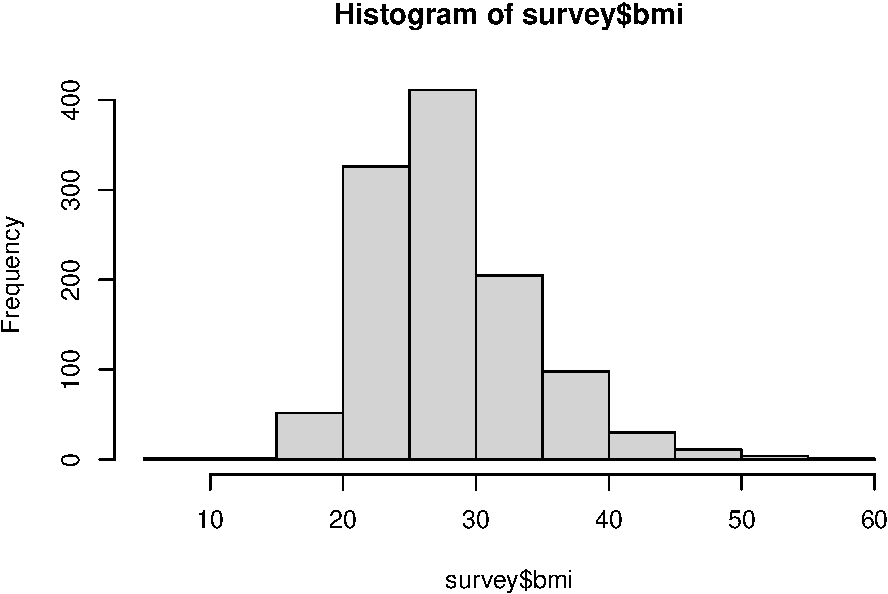
\includegraphics{phcm9795-R-notes_files/figure-latex/unnamed-chunk-64-1.pdf}

\begin{Shaded}
\begin{Highlighting}[]
\FunctionTok{boxplot}\NormalTok{(survey}\SpecialCharTok{$}\NormalTok{bmi)}
\end{Highlighting}
\end{Shaded}

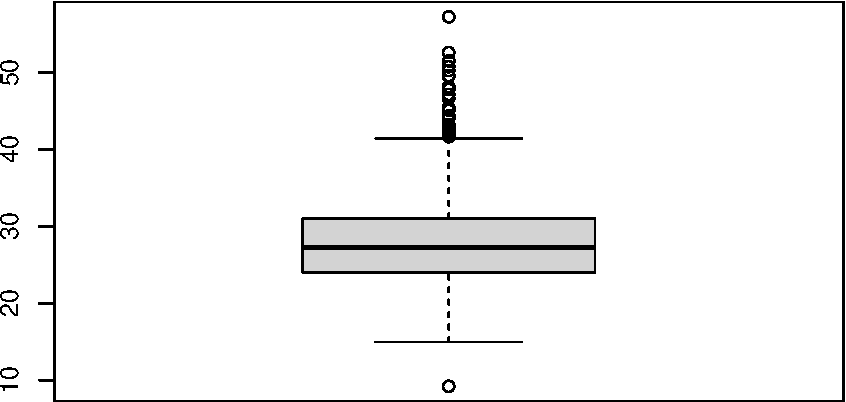
\includegraphics{phcm9795-R-notes_files/figure-latex/unnamed-chunk-64-2.pdf}

In the general population, BMI ranges between about 15 to 30. It appears that BMI has been correctly generated in this example. We should investigate the very low and some of the very high values of BMI, but this will be left for another time.

\hypertarget{summarising-data-by-another-variable}{%
\section{Summarising data by another variable}\label{summarising-data-by-another-variable}}

We will often want to calculate the same summary statistics by another variable. For example, we might want to calculate summary statistics for BMI for males and females separately. We can do this in in the \texttt{descriptives} function by defining sex as a \texttt{splitBy} variable:

\begin{Shaded}
\begin{Highlighting}[]
\FunctionTok{library}\NormalTok{(jmv)}
\FunctionTok{descriptives}\NormalTok{(}\AttributeTok{data=}\NormalTok{survey, }\AttributeTok{vars=}\NormalTok{bmi, }\AttributeTok{splitBy =}\NormalTok{ sex)}
\end{Highlighting}
\end{Shaded}

\begin{verbatim}
## 
##  DESCRIPTIVES
## 
##  Descriptives                                 
##  ──────────────────────────────────────────── 
##                          sex       bmi        
##  ──────────────────────────────────────────── 
##    N                     Male           513   
##                          Female         627   
##    Missing               Male             0   
##                          Female           0   
##    Mean                  Male      28.29561   
##                          Female    27.81434   
##    Median                Male      27.39592   
##                          Female    26.66667   
##    Standard deviation    Male      5.204975   
##                          Female    6.380523   
##    Minimum               Male      16.47519   
##                          Female    9.209299   
##    Maximum               Male      57.23644   
##                          Female    52.59516   
##  ────────────────────────────────────────────
\end{verbatim}

\hypertarget{summarising-a-single-column-of-data}{%
\section{Summarising a single column of data}\label{summarising-a-single-column-of-data}}

In Module 1, we started with a very simple analysis: reading in six ages, and them using \texttt{summary()} to calculate descriptive statistics. We then went on to use the \texttt{decriptives()} function in the \texttt{jmv} package as more flexible way of calculating descriptive statistics. Let's revisit this analysis:

\begin{Shaded}
\begin{Highlighting}[]
\CommentTok{\# Author: Timothy Dobbins}
\CommentTok{\# Date: 5 April 2022}
\CommentTok{\# Purpose: My first R script}
\FunctionTok{library}\NormalTok{(jmv)}

\NormalTok{age }\OtherTok{\textless{}{-}} \FunctionTok{c}\NormalTok{(}\DecValTok{20}\NormalTok{, }\DecValTok{25}\NormalTok{, }\DecValTok{23}\NormalTok{, }\DecValTok{29}\NormalTok{, }\DecValTok{21}\NormalTok{, }\DecValTok{27}\NormalTok{)}

\CommentTok{\# Use "summary" to obtain descriptive statistics}
\FunctionTok{summary}\NormalTok{(age)}
\end{Highlighting}
\end{Shaded}

\begin{verbatim}
##    Min. 1st Qu.  Median    Mean 3rd Qu.    Max. 
##   20.00   21.50   24.00   24.17   26.50   29.00
\end{verbatim}

\begin{Shaded}
\begin{Highlighting}[]
\CommentTok{\# Use "descriptives" to obtain descriptive statistics}
\FunctionTok{descriptives}\NormalTok{(age)}
\end{Highlighting}
\end{Shaded}

\begin{verbatim}
## Error: Argument 'data' must be a data frame
\end{verbatim}

The \texttt{summary()} function has worked correctly, but the \texttt{descriptives()} function has given an error: \texttt{Error:\ Argument\ \textquotesingle{}data\textquotesingle{}\ must\ be\ a\ data\ frame}. What on earth is going on here?

The error gives us a clue here - the \texttt{descriptives()} function requires a data frame for analysis. We have provided the object \texttt{age}: a \textbf{vector}. As we saw in Section \ref{data-structures}, a vector is a single column of data, while a data frame is a collection of columns.

In order to summarise a vector using the \texttt{descriptives()} function, we must first convert the vector into a data frame using \texttt{as.data.frame()}. For example:

\begin{Shaded}
\begin{Highlighting}[]
\CommentTok{\# Author: Timothy Dobbins}
\CommentTok{\# Date: 5 April 2022}
\CommentTok{\# Purpose: My first R script}
\FunctionTok{library}\NormalTok{(jmv)}

\NormalTok{age }\OtherTok{\textless{}{-}} \FunctionTok{c}\NormalTok{(}\DecValTok{20}\NormalTok{, }\DecValTok{25}\NormalTok{, }\DecValTok{23}\NormalTok{, }\DecValTok{29}\NormalTok{, }\DecValTok{21}\NormalTok{, }\DecValTok{27}\NormalTok{)}

\CommentTok{\# Use "summary" to obtain descriptive statistics}
\FunctionTok{summary}\NormalTok{(age)}
\end{Highlighting}
\end{Shaded}

\begin{verbatim}
##    Min. 1st Qu.  Median    Mean 3rd Qu.    Max. 
##   20.00   21.50   24.00   24.17   26.50   29.00
\end{verbatim}

\begin{Shaded}
\begin{Highlighting}[]
\CommentTok{\# Create a new data frame from the vector age:}

\NormalTok{age\_df }\OtherTok{\textless{}{-}} \FunctionTok{as.data.frame}\NormalTok{(age)}

\CommentTok{\# Use "descriptives" to obtain descriptive statistics for age\_df}
\FunctionTok{descriptives}\NormalTok{(age\_df)}
\end{Highlighting}
\end{Shaded}

\begin{verbatim}
## 
##  DESCRIPTIVES
## 
##  Descriptives                       
##  ────────────────────────────────── 
##                          age        
##  ────────────────────────────────── 
##    N                            6   
##    Missing                      0   
##    Mean                  24.16667   
##    Median                24.00000   
##    Standard deviation    3.488075   
##    Minimum               20.00000   
##    Maximum               29.00000   
##  ──────────────────────────────────
\end{verbatim}

\hypertarget{plotting-data-by-another-variable}{%
\section{Plotting data by another variable}\label{plotting-data-by-another-variable}}

Unfortunately, it is not straight-forward to create separate plots for every level of another variable. We will demonstrate by plotting BMI by sex using our health survey data.

The following steps are not the most efficient way of doing this, but are easy to follow and understand. We first begin by creating two new data frames, for males and females separately, using the \texttt{subset()} function:

\begin{Shaded}
\begin{Highlighting}[]
\NormalTok{survey\_males }\OtherTok{\textless{}{-}} \FunctionTok{subset}\NormalTok{(survey, sex}\SpecialCharTok{==}\StringTok{"Male"}\NormalTok{)}
\NormalTok{survey\_females }\OtherTok{\textless{}{-}} \FunctionTok{subset}\NormalTok{(survey, sex}\SpecialCharTok{==}\StringTok{"Female"}\NormalTok{)}
\end{Highlighting}
\end{Shaded}

Note that we use the \textbf{label} for sex, not the underlying numeric value, as sex is a \textbf{factor}.

We can now create hisotgrams and boxplots of BMI for males and females separately. To place the graphs next to each other in a single figure, we can use the \texttt{par} function, which sets the \emph{graphics parameters}. Essentially, we want to tell R to split a plot window into a matrix with \emph{nr} rows and \emph{nc} columns, and we fill the cells by rows (\texttt{mfrow}) or columns (\texttt{mfcols}).

For example, to plot four figures in a single plot, filled by rows, we use \texttt{par(mfrow=c(2,2))}.

When we are done plotting multiple graphs, we can reset the graphics parameters by submitting \texttt{par(mfrow=c(1,1))}.

\begin{Shaded}
\begin{Highlighting}[]
\CommentTok{\# Set the graphics parameters to plot 2 rows and 2 columns:}
\FunctionTok{par}\NormalTok{(}\AttributeTok{mfrow=}\FunctionTok{c}\NormalTok{(}\DecValTok{2}\NormalTok{,}\DecValTok{2}\NormalTok{))}

\CommentTok{\# Specify each plot separately}
\FunctionTok{hist}\NormalTok{(survey\_males}\SpecialCharTok{$}\NormalTok{bmi, }\AttributeTok{xlab=}\StringTok{"BMI (kg/m2)"}\NormalTok{, }\AttributeTok{main=}\StringTok{"Males"}\NormalTok{)}
\FunctionTok{hist}\NormalTok{(survey\_females}\SpecialCharTok{$}\NormalTok{bmi, }\AttributeTok{xlab=}\StringTok{"BMI (kg/m2)"}\NormalTok{, }\AttributeTok{main=}\StringTok{"Females"}\NormalTok{)}

\FunctionTok{boxplot}\NormalTok{(survey\_males}\SpecialCharTok{$}\NormalTok{bmi, }\AttributeTok{ylab=}\StringTok{"BMI (kg/m2)"}\NormalTok{, }\AttributeTok{main=}\StringTok{"Males"}\NormalTok{)}
\FunctionTok{boxplot}\NormalTok{(survey\_females}\SpecialCharTok{$}\NormalTok{bmi, }\AttributeTok{ylab=}\StringTok{"BMI (kg/m2)"}\NormalTok{, }\AttributeTok{main=}\StringTok{"Females"}\NormalTok{)}
\end{Highlighting}
\end{Shaded}

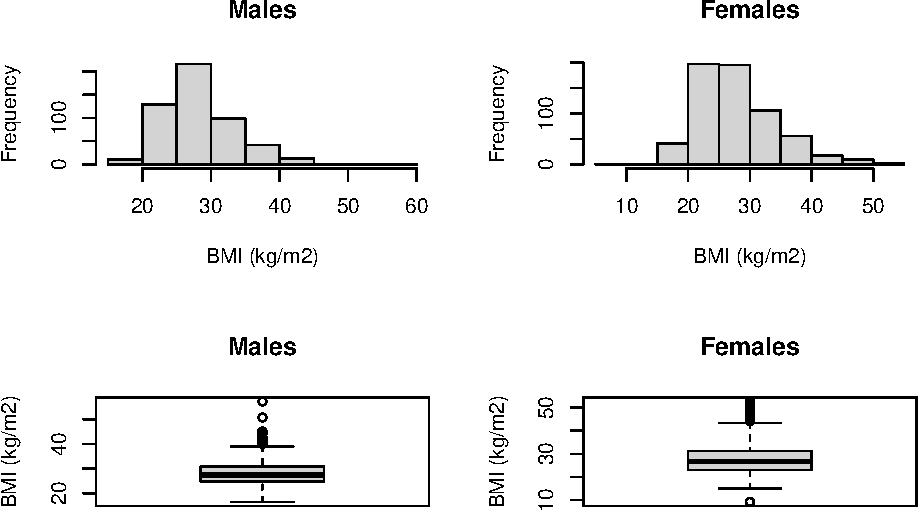
\includegraphics{phcm9795-R-notes_files/figure-latex/unnamed-chunk-70-1.pdf}

\begin{Shaded}
\begin{Highlighting}[]
\CommentTok{\# Reset graphics parameters}
\FunctionTok{par}\NormalTok{(}\AttributeTok{mfrow=}\FunctionTok{c}\NormalTok{(}\DecValTok{1}\NormalTok{,}\DecValTok{1}\NormalTok{))}
\end{Highlighting}
\end{Shaded}

\hypertarget{recoding-data}{%
\section{Recoding data}\label{recoding-data}}

One task that is common in statistical computing is to recode variables. For example, we might want to group some categories of a categorical variable, or to present a continuous variable in a categorical way.

In this example, we can recode BMI into the following categories as suggested by the World Health Organisation {[}footnote{]}:

\begin{itemize}
\tightlist
\item
  Underweight: BMI \textless{} 18.5
\item
  Normal weight: 18.5 \(\le\) BMI \textless{} 25
\item
  Pre-obesity: 25 \(\le\) BMI \textless{} 30
\item
  Obesity Class I: 30 \(\le\) BMI \textless{} 35
\item
  Obesity Class II: 35 \(\le\) BMI \textless{} 40
\item
  Obesity Class III: BMI \(\ge\) 40
\end{itemize}

The quickest way to recode a continuous variable into categories is to use the \texttt{cut} command which takes a continuous variable, and ``cuts'' it into groups based on the specified ``cutpoints''

\begin{Shaded}
\begin{Highlighting}[]
\NormalTok{survey}\SpecialCharTok{$}\NormalTok{bmi\_cat }\OtherTok{\textless{}{-}} \FunctionTok{cut}\NormalTok{(survey}\SpecialCharTok{$}\NormalTok{bmi, }
                      \AttributeTok{breaks =} \FunctionTok{c}\NormalTok{(}\DecValTok{0}\NormalTok{, }\FloatTok{18.5}\NormalTok{, }\DecValTok{25}\NormalTok{, }\DecValTok{30}\NormalTok{, }\DecValTok{35}\NormalTok{, }\DecValTok{40}\NormalTok{, }\DecValTok{100}\NormalTok{))}
\end{Highlighting}
\end{Shaded}

Notice that lower (BMI=0) and upper (BMI=100) bounds have been specified, as both a lower and upper limit must be defined for each group.

If we examine the new \texttt{bmi\_cat} variable:

\begin{Shaded}
\begin{Highlighting}[]
\FunctionTok{summary}\NormalTok{(survey}\SpecialCharTok{$}\NormalTok{bmi\_cat)}
\end{Highlighting}
\end{Shaded}

\begin{verbatim}
##  (0,18.5] (18.5,25]   (25,30]   (30,35]   (35,40]  (40,100] 
##        18       362       411       205        97        47
\end{verbatim}

we see that each group has been labelled (a, b{]}. This notation is equivalent to: greater than a, and less than or equal to b. The \texttt{cut} function excludes the lower limit, but includes the upper limit. Our BMI ranges have been defined to include the lower limit, and exclude the upper limit (for example, greater than or equal to 30 and less than 35).

We can specify this recoding using the \texttt{right=FALSE} option:

\begin{Shaded}
\begin{Highlighting}[]
\NormalTok{survey}\SpecialCharTok{$}\NormalTok{bmi\_cat }\OtherTok{\textless{}{-}} \FunctionTok{cut}\NormalTok{(survey}\SpecialCharTok{$}\NormalTok{bmi,}
                      \AttributeTok{breaks =} \FunctionTok{c}\NormalTok{(}\DecValTok{0}\NormalTok{, }\FloatTok{18.5}\NormalTok{, }\DecValTok{25}\NormalTok{, }\DecValTok{30}\NormalTok{, }\DecValTok{35}\NormalTok{, }\DecValTok{40}\NormalTok{, }\DecValTok{100}\NormalTok{),}
                      \AttributeTok{right=}\ConstantTok{FALSE}\NormalTok{)}

\FunctionTok{summary}\NormalTok{(survey}\SpecialCharTok{$}\NormalTok{bmi\_cat)}
\end{Highlighting}
\end{Shaded}

\begin{verbatim}
##  [0,18.5) [18.5,25)   [25,30)   [30,35)   [35,40)  [40,100) 
##        18       362       411       201       101        47
\end{verbatim}

Finally, we can specify labels for the groups using the \texttt{labels} option:

\begin{Shaded}
\begin{Highlighting}[]
\NormalTok{survey}\SpecialCharTok{$}\NormalTok{bmi\_cat }\OtherTok{\textless{}{-}} \FunctionTok{cut}\NormalTok{(survey}\SpecialCharTok{$}\NormalTok{bmi,}
                      \AttributeTok{breaks =} \FunctionTok{c}\NormalTok{(}\DecValTok{0}\NormalTok{, }\FloatTok{18.5}\NormalTok{, }\DecValTok{25}\NormalTok{, }\DecValTok{30}\NormalTok{, }\DecValTok{35}\NormalTok{, }\DecValTok{40}\NormalTok{, }\DecValTok{100}\NormalTok{),}
                      \AttributeTok{right=}\ConstantTok{FALSE}\NormalTok{,}
                      \AttributeTok{labels =} \FunctionTok{c}\NormalTok{(}\StringTok{"Underweight"}\NormalTok{, }\StringTok{"Normal"}\NormalTok{, }\StringTok{"Pre{-}obesity"}\NormalTok{,}
                                 \StringTok{"Obesity Class I"}\NormalTok{, }\StringTok{"Obesity Class II"}\NormalTok{,}
                                 \StringTok{"Obesity Class III"}\NormalTok{))}

\FunctionTok{summary}\NormalTok{(survey}\SpecialCharTok{$}\NormalTok{bmi\_cat)}
\end{Highlighting}
\end{Shaded}

\begin{verbatim}
##       Underweight            Normal       Pre-obesity   Obesity Class I 
##                18               362               411               201 
##  Obesity Class II Obesity Class III 
##               101                47
\end{verbatim}

\hypertarget{computing-binomial-probabilities-using-r}{%
\section{Computing binomial probabilities using R}\label{computing-binomial-probabilities-using-r}}

There are two R functions that we can use to calculate probabilities based on the binomial distribution: \texttt{dbinom} and \texttt{pbinom}:

\begin{itemize}
\tightlist
\item
  \texttt{dbinom(x,\ size,\ prob)} gives the probability of obtaining \texttt{x} successes from \texttt{size} trials when the probability of a success on one trial is \texttt{prob};
\item
  \texttt{pbinom(q,\ size,\ prob)} gives the probability of obtaining \texttt{q} \textbf{or fewer} successes from \texttt{size} trials when the probability of a success on one trial is \texttt{prob};
\item
  \texttt{pbinom(q,\ size,\ prob,\ lower.tail=FALSE)} gives the probability of obtaining \textbf{more than} \texttt{q}successes from \texttt{size} trials when the probability of a success on one trial is \texttt{prob}.
\end{itemize}

To do the computation for part (a) in Worked Example 2.1, we will use the \texttt{dbinom} function with:

\begin{itemize}
\tightlist
\item
  \emph{x} is the number of successes, here, the number of smokers (i.e.~k=3);
\item
  \emph{size} is the number of trials (i.e.~n=6);
\item
  and \emph{prob} is probability of drawing a smoker from the population, which is 19.8\% (i.e.~p=0.198).
\end{itemize}

Replace each of these with the appropriate number into the formula:

\begin{Shaded}
\begin{Highlighting}[]
\FunctionTok{dbinom}\NormalTok{(}\AttributeTok{x=}\DecValTok{3}\NormalTok{, }\AttributeTok{size=}\DecValTok{6}\NormalTok{, }\AttributeTok{prob=}\FloatTok{0.198}\NormalTok{)}
\end{Highlighting}
\end{Shaded}

\begin{verbatim}
## [1] 0.08008454
\end{verbatim}

To calculate the upper tail of probability in part (b), we use the \texttt{pbinom(lower.tail=FALSE)} function. Note that the \texttt{pbinom(lower.tail=FALSE)} function \textbf{does not include \texttt{q}}, so to obtain 4 or more successes, we need to enter \texttt{q=3}:

\begin{Shaded}
\begin{Highlighting}[]
\FunctionTok{pbinom}\NormalTok{(}\AttributeTok{q=}\DecValTok{3}\NormalTok{, }\AttributeTok{size=}\DecValTok{6}\NormalTok{, }\AttributeTok{prob=}\FloatTok{0.198}\NormalTok{, }\AttributeTok{lower.tail=}\ConstantTok{FALSE}\NormalTok{)}
\end{Highlighting}
\end{Shaded}

\begin{verbatim}
## [1] 0.01635325
\end{verbatim}

For the lower tail for part (c), we use the \texttt{pbinom} function:

\begin{Shaded}
\begin{Highlighting}[]
\FunctionTok{pbinom}\NormalTok{(}\AttributeTok{q=}\DecValTok{2}\NormalTok{, }\AttributeTok{size=}\DecValTok{6}\NormalTok{, }\AttributeTok{prob=}\FloatTok{0.198}\NormalTok{)}
\end{Highlighting}
\end{Shaded}

\begin{verbatim}
## [1] 0.9035622
\end{verbatim}

\hypertarget{computing-probabilities-from-a-normal-distribution}{%
\section{Computing probabilities from a Normal distribution}\label{computing-probabilities-from-a-normal-distribution}}

We can use the \texttt{pnorm} function to calculate probabilities from a Normal distribution:

\begin{itemize}
\tightlist
\item
  \texttt{pnorm(q,\ mean,\ sd)} calculates the probability of observing a value of \texttt{q} or less, from a Normal distribution with a mean of \texttt{mean} and a standard deviation of \texttt{sd}. Note that if \texttt{mean} and \texttt{sd} are not entered, they are assumed to be 0 and 1 respectively (i.e.~a standard normal distribution.)
\item
  \texttt{pnorm(q,\ mean,\ sd,\ lower.tail=FALSE)} calculates the probability of observing a value of more than \texttt{q}, from a Normal distribution with a mean of \texttt{mean} and a standard deviation of \texttt{sd}.
\end{itemize}

To obtain the probability of obtaining 0.5 or greater from a standard normal distribution:

\begin{Shaded}
\begin{Highlighting}[]
\FunctionTok{pnorm}\NormalTok{(}\FloatTok{0.5}\NormalTok{, }\AttributeTok{lower.tail=}\ConstantTok{FALSE}\NormalTok{)}
\end{Highlighting}
\end{Shaded}

\begin{verbatim}
## [1] 0.3085375
\end{verbatim}

To calculate the worked example: Assume that the mean diastolic blood pressure for men is 77.9 mmHg, with a standard deviation of 11. What is the probability that a man selected at random will have high blood pressure (i.e.~diastolic blood pressure greater than or equal to 90)?

\begin{Shaded}
\begin{Highlighting}[]
\FunctionTok{pnorm}\NormalTok{(}\DecValTok{90}\NormalTok{, }\AttributeTok{mean=}\FloatTok{77.9}\NormalTok{, }\AttributeTok{sd=}\DecValTok{11}\NormalTok{, }\AttributeTok{lower.tail=}\ConstantTok{FALSE}\NormalTok{)}
\end{Highlighting}
\end{Shaded}

\begin{verbatim}
## [1] 0.1356661
\end{verbatim}

\hypertarget{precision-r-notes}{%
\chapter{Precision: R notes}\label{precision-r-notes}}

\hypertarget{calculating-a-95-confidence-interval-of-a-mean}{%
\section{Calculating a 95\% confidence interval of a mean}\label{calculating-a-95-confidence-interval-of-a-mean}}

\hypertarget{individual-data}{%
\subsection{Individual data}\label{individual-data}}

To demonstrate the computation of the 95\% confidence interval of a mean we have used data from \texttt{Example\_1.3.rds} which contains the weights of 30 students:

\begin{Shaded}
\begin{Highlighting}[]
\FunctionTok{library}\NormalTok{(jmv)}

\NormalTok{students }\OtherTok{\textless{}{-}} \FunctionTok{readRDS}\NormalTok{(}\StringTok{"data/examples/Example\_1.3.rds"}\NormalTok{)}

\FunctionTok{summary}\NormalTok{(students)}
\end{Highlighting}
\end{Shaded}

\begin{verbatim}
##      weight         gender  
##  Min.   :60.00   Male  :16  
##  1st Qu.:67.50   Female:14  
##  Median :70.00              
##  Mean   :70.00              
##  3rd Qu.:74.38              
##  Max.   :80.00
\end{verbatim}

The mean and its 95\% confidence interval can be obtained many ways in R. We will use the \texttt{t.test()} function installed in R to calculate the confidence interval:

\begin{Shaded}
\begin{Highlighting}[]
\FunctionTok{t.test}\NormalTok{(students}\SpecialCharTok{$}\NormalTok{weight)}
\end{Highlighting}
\end{Shaded}

\begin{verbatim}
## 
##  One Sample t-test
## 
## data:  students$weight
## t = 76.029, df = 29, p-value < 2.2e-16
## alternative hypothesis: true mean is not equal to 0
## 95 percent confidence interval:
##  68.11694 71.88306
## sample estimates:
## mean of x 
##        70
\end{verbatim}

The output of the \texttt{t.test()} function gives us the sample mean (70.0 kg) as well as the 95\% confidence interval around the mean: 68.1 to 71.9 kg.

Note: the \texttt{descriptives()} function within the \texttt{jmv} package also calculates a 95\% confidence interval around the mean. \textbf{It is recommended not to use this function} as it currently (as of June 2022) uses a \emph{z} value to calculate the confidence interval, rather than a \emph{t} value.

\hypertarget{summarised-data}{%
\subsection{Summarised data}\label{summarised-data}}

For Worked Example 3.2 where we are given the sample mean, sample standard deviation and sample size. R does not have a built-in function to calculate a confidence interval from summarised data, but we can write our own.

\textbf{Note: writing your own functions is beyond the scope of this course. You should copy and paste the code provided to do this.}

\begin{Shaded}
\begin{Highlighting}[]
\DocumentationTok{\#\#\# Copy this section}
\NormalTok{ci\_mean }\OtherTok{\textless{}{-}} \ControlFlowTok{function}\NormalTok{(n, mean, sd, }\AttributeTok{width=}\FloatTok{0.95}\NormalTok{, }\AttributeTok{digits=}\DecValTok{3}\NormalTok{)\{}
\NormalTok{  lcl }\OtherTok{\textless{}{-}}\NormalTok{ mean }\SpecialCharTok{{-}} \FunctionTok{qt}\NormalTok{(}\AttributeTok{p=}\NormalTok{(}\DecValTok{1} \SpecialCharTok{{-}}\NormalTok{ (}\DecValTok{1}\SpecialCharTok{{-}}\NormalTok{width)}\SpecialCharTok{/}\DecValTok{2}\NormalTok{), }\AttributeTok{df=}\NormalTok{n}\DecValTok{{-}1}\NormalTok{) }\SpecialCharTok{*}\NormalTok{ sd}\SpecialCharTok{/}\FunctionTok{sqrt}\NormalTok{(n)}
\NormalTok{  ucl }\OtherTok{\textless{}{-}}\NormalTok{ mean }\SpecialCharTok{+} \FunctionTok{qt}\NormalTok{(}\AttributeTok{p=}\NormalTok{(}\DecValTok{1} \SpecialCharTok{{-}}\NormalTok{ (}\DecValTok{1}\SpecialCharTok{{-}}\NormalTok{width)}\SpecialCharTok{/}\DecValTok{2}\NormalTok{), }\AttributeTok{df=}\NormalTok{n}\DecValTok{{-}1}\NormalTok{) }\SpecialCharTok{*}\NormalTok{ sd}\SpecialCharTok{/}\FunctionTok{sqrt}\NormalTok{(n)}
  
  \FunctionTok{print}\NormalTok{(}\FunctionTok{paste0}\NormalTok{(width}\SpecialCharTok{*}\DecValTok{100}\NormalTok{, }\StringTok{"\%"}\NormalTok{, }\StringTok{" CI: "}\NormalTok{, }\FunctionTok{format}\NormalTok{(}\FunctionTok{round}\NormalTok{(lcl, }\AttributeTok{digits=}\NormalTok{digits), }\AttributeTok{nsmall =}\NormalTok{ digits),}
               \StringTok{" to "}\NormalTok{, }\FunctionTok{format}\NormalTok{(}\FunctionTok{round}\NormalTok{(ucl, }\AttributeTok{digits=}\NormalTok{digits), }\AttributeTok{nsmall =}\NormalTok{ digits) ))}

\NormalTok{\}}
\DocumentationTok{\#\#\# End of copy}

\FunctionTok{ci\_mean}\NormalTok{(}\AttributeTok{n=}\DecValTok{30}\NormalTok{, }\AttributeTok{mean=}\DecValTok{70}\NormalTok{, }\AttributeTok{sd=}\DecValTok{6}\NormalTok{, }\AttributeTok{width=}\FloatTok{0.95}\NormalTok{)}
\end{Highlighting}
\end{Shaded}

\begin{verbatim}
## [1] "95% CI: 67.760 to 72.240"
\end{verbatim}

\begin{Shaded}
\begin{Highlighting}[]
\FunctionTok{ci\_mean}\NormalTok{(}\AttributeTok{n=}\DecValTok{30}\NormalTok{, }\AttributeTok{mean=}\DecValTok{70}\NormalTok{, }\AttributeTok{sd=}\DecValTok{6}\NormalTok{, }\AttributeTok{width=}\FloatTok{0.99}\NormalTok{)}
\end{Highlighting}
\end{Shaded}

\begin{verbatim}
## [1] "99% CI: 66.981 to 73.019"
\end{verbatim}

\hypertarget{hypothesis-testing}{%
\chapter{Hypothesis testing}\label{hypothesis-testing}}

\hypertarget{one-sample-t-test}{%
\section{One sample t-test}\label{one-sample-t-test}}

We will use data from \texttt{Example\_4.1.rds} to demonstrate how a one-sample t-test is conducted in R.

\begin{Shaded}
\begin{Highlighting}[]
\NormalTok{bloodpressure }\OtherTok{\textless{}{-}} \FunctionTok{readRDS}\NormalTok{(}\StringTok{"data/examples/Example\_4.1.rds"}\NormalTok{)}

\FunctionTok{summary}\NormalTok{(bloodpressure)}
\end{Highlighting}
\end{Shaded}

\begin{verbatim}
##       dbp        
##  Min.   : 24.00  
##  1st Qu.: 64.00  
##  Median : 72.00  
##  Mean   : 72.41  
##  3rd Qu.: 80.00  
##  Max.   :122.00  
##  NA's   :35
\end{verbatim}

To test whether the mean diastolic blood pressure of the population from which the sample was drawn is equal to 71, we can use the t.test command:

\begin{Shaded}
\begin{Highlighting}[]
\FunctionTok{t.test}\NormalTok{(bloodpressure}\SpecialCharTok{$}\NormalTok{dbp, }\AttributeTok{mu=}\DecValTok{71}\NormalTok{)}
\end{Highlighting}
\end{Shaded}

\begin{verbatim}
## 
##  One Sample t-test
## 
## data:  bloodpressure$dbp
## t = 3.0725, df = 732, p-value = 0.002202
## alternative hypothesis: true mean is not equal to 71
## 95 percent confidence interval:
##  71.50732 73.30305
## sample estimates:
## mean of x 
##  72.40518
\end{verbatim}

The output gives a test statistic, degrees of freedom and a P values from the two-sided test. The mean of the sample is provided, as well as the 95\% confidence interval.

  \bibliography{PHCM9795.bib}

\end{document}
